%!TEX encoding = UTF-8 Unicode
% options:
% thesis=B bachelor's thesis
% thesis=M master's thesis
% czech thesis in Czech language
% slovak thesis in Slovak language
% english thesis in English language
% hidelinks remove colour boxes around hyperlinks

\documentclass[thesis=M,czech]{FITthesis}[2012/06/26]

\usepackage[utf8]{inputenc} % LaTeX source encoded as UTF-8

\usepackage{graphicx} %graphics files inclusion
\graphicspath{ {img/} }
\usepackage{amsmath} %advanced maths
% \usepackage{amssymb} %additional math symbols


\usepackage{parcolumns}
\usepackage{caption}
\usepackage{subcaption}
\usepackage{listings}
\usepackage{minted}

\usepackage{dirtree} %directory tree visualisation

% % list of acronyms
% \usepackage[acronym,nonumberlist,toc,numberedsection=autolabel]{glossaries}
% \iflanguage{czech}{\renewcommand*{\acronymname}{Seznam pou{\v z}it{\' y}ch zkratek}}{}
% \makeglossaries

\newcommand{\tg}{\mathop{\mathrm{tg}}} %cesky tangens
\newcommand{\cotg}{\mathop{\mathrm{cotg}}} %cesky cotangens

% % % % % % % % % % % % % % % % % % % % % % % % % % % % % % 
% ODTUD DAL VSE ZMENTE
% % % % % % % % % % % % % % % % % % % % % % % % % % % % % % 

\department{Katedra Webové a softwarové inženýrství}
\title{Hledání a využití struktury multimediálních dat}
\authorGN{Doplňte Vaše křestní jméno/jména} %(křestní) jméno (jména) autora
\authorFN{Doplňte Vaše příjmení} %příjmení autora
\authorWithDegrees{Doplňte Vaše jméno a tituly} %jméno autora včetně současných akademických titulů
\supervisor{Doplňte jméno vedoucího práce}
\acknowledgements{Doplňte, máte-li komu a za co děkovat. V~opačném případě úplně odstraňte tento příkaz.}
\abstractCS{V~několika větách shrňte obsah a přínos této práce v~češtině. Po přečtení abstraktu by se čtenář měl mít čtenář dost informací pro rozhodnutí, zda chce Vaši práci číst.}
\abstractEN{Sem doplňte ekvivalent abstraktu Vaší práce v~angličtině.}
\placeForDeclarationOfAuthenticity{V~Praze}
\declarationOfAuthenticityOption{4} %volba Prohlášení (číslo 1-6)
\keywordsCS{Nahraďte seznamem klíčových slov v češtině oddělených čárkou.}
\keywordsEN{Nahraďte seznamem klíčových slov v angličtině oddělených čárkou.}

\begin{document}
\renewcommand\listingscaption{Ukázka}
\definecolor{bg}{rgb}{0.95,0.95,0.95}
% \newacronym{CVUT}{{\v C}VUT}{{\v C}esk{\' e} vysok{\' e} u{\v c}en{\' i} technick{\' e} v Praze}
% \newacronym{FIT}{FIT}{Fakulta informa{\v c}n{\' i}ch technologi{\' i}}

\begin{introduction}

\textit{Struktura} (z latinského struere, skládat, sestavovat, budovat, pořádat) označuje způsob složení, vnitřního uspořádání nějakého objektu, zejména pokud vykazuje nějaké pravidelnosti a zákonitosti. Existuje několik možných jak hledat strukturu v datech ... TODO
V této práci bude struktura hledána pomocí \textit{shlukování}, což je analýza, která má za úkol najít homogenní skupiny objektů. 

Struktury budou hledány v kolekcích skladeb populární hudby, jako představiteli multimediálních dat \cite{multimedia}. 

Společné rysy takových dat: (nemá strukturu ve smyslu....) TODO


Nejen pro interpretaci výsledků jsou nutné expertní znalosti z domény. Nicméně výhodou populární hudby je právě její rozšířenost mezi širší publikum, kde každý posluchač intuitivně snadno určí podobnost dvou skladeb nebo interpretů a jestli se mu konkrétní hudba líbí, nebo ne. 




Je potřeba expert (vždy)
Proč byly zvoleny: netriviální objekty, shlukování je na základě podobnosti, každý hudební nadšenec je schopen porovnat dvě skladby a určit intuitivní míru podobnosti. Zároveň je velmi obtížné zachytit tyto "oblíbené" znaky. Předpovídat atd,.  s pomocí počítačů


- celé KDD
- zvolené metody (vizuální extrakce shluků)
- sémantický kontext


- využití


	%sem napište úvod Vaší práce
	
	\section{Cíl práce}
	
	vyzkoušet možnosti hledání shluků pomocí SOM a CRSOM
\end{introduction}

% POUŽITÉ METODY -------------------------------------------------------------------------------------------------------------------------------------------------------------------------------------------------------------
\chapter{Použité metody}
\section{Dobývání znalostí z databází (KDD)}
\textit{Dobývání znalostí z databází (Knowledge discovery in databases, KDD)} představuje netriviální extrakci nových a reálně využitelných znalostí z dat\cite{kddb}. 

Cílem KDD je získat cenné nové informace, které nebyly z neopracovaných dat explicitně viditelné a vhodným způsobem a formou pak tyto informace zobrazit, popřípadě využít v reálných systémech.\cite{fayyad}

KDD se dá popsat jako proces skládající se z několika kroků. Tyto kroky se zpravidla iterativně opakují a některé vyžadují vysokou interakci uživatele. Kroky KDD, tak jak jsou popsány v \cite{hbcap}, jsou následující:

\begin{figure}[htbp]
\begin{center}
	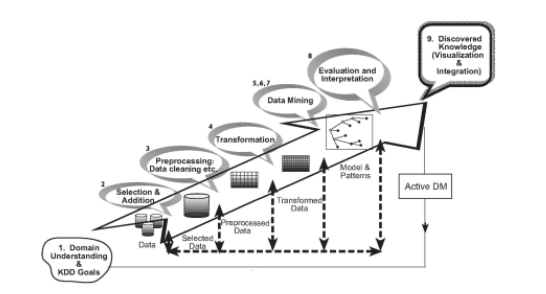
\includegraphics[scale=0.75]{kdd_steps}
\caption{Kroky KDD podle \cite{fayyad}}
\end{center}
 \captionsetup{font={footnotesize,bf,it}}
  \caption*{zdroj: \cite{fayyad}}
\end{figure}

\subsubsection*{Porozumění aplikační doméně a stanovení cílů}
Částí počátečního kroku je důkladně poznat aplikační doménu. Další kritickou částí je stanovení cílů, které by KDD měly přinést koncovému uživateli. Tato rozhodnutí pak významným způsobem ovlivňují jednotlivá rozhodnutí v dalších krocích.
 		
\subsubsection*{Výběr dat}
Potom, co je specifikován cíl, je zapotřebí rozhodnout z jakých dat se budou znalosti dobývat. 
Výsledkem tohoto kroku je vstupní množina dat, která velmi ovlivňuje úspěch celého KDD. Pokud například budou chybět některé významné atributy, s ohledem na stanovený cíl, celý proces pravděpodobně nebude úspěšný. Z tohoto pohledu je dobré zahrnout co nejvíce různých atributů. Na druhou stranu s velikostí dat se zvyšuje výpočetní a prostorová náročnost napříč metodami ze všech následujících kroků. Tyto protichůdné požadavky je třeba zvážit a udělat kompromis. Správnému rozhodnutí by měla pomoci iterativní povaha celého procesu.

\subsubsection*{Předzpracování}
Tento krok má za cíl zvýšit kvalitu dat. Předzpracování by se mělo například vypořádat s chybějícími a odlehlými hodnotami. Nejen v tomto kroku platí \uv{\emph{garbage in garbage out}}, koncept běžný pro počítačové vědy a matematiku, který stojí na myšlence, že kvalita výstupu je určena kvalitou vstupu\cite{g_in_g_out}.

\subsubsection*{Transformace }
\label{subsec:transformace}

V této části KDD se používají metody na transformaci atributů, jako je například diskretizace. Dále se v tomto kroku může měnit dimenzionalita dat a to buď zmenšovat metodami jako \textit{feature selection, feature extraction}, nebo naopak zvětšovat odvozovováním atributů nových. 


\subsubsection*{Datamining}
Před tímto krokem bychom měli mít k dispozici připravená data. Jak již bylo ovšem zmíněno, celý process KDD je iterativní a tento krok lze provádět s různými datovými sadami a výsedky vzájemně porovnávat.

Ze stanoveného cíle KDD jsou odvozeny kritéria pro zvolení vhodných dataminingových metod. Zvolené metody se poté aplikují na připravená data. Výsledkem tohoto kroku může být natrénovaný model nebo sada extrahovaných znalostí.

\subsubsection*{Vyhodnocení a interpretace}
V této časti máme již natrénované modely, popřípadě extrahované znalosti. Tyto výsledky musíme vyhodnotit a interpretovat z hlediska cílů, které byly stanoveny v prvním kroku.

\subsubsection*{Využití}
Využití je posledním krokem celého KDD. Získané znalosti jsou využity v reálných systémech a natrénované modely jsou nasazeny do produčního prostředí. Tento krok se snaží přinést užitek koncovému uživateli. Úspěch tohoto kroku definuje úspěch celého KDD.	
	

\subsection{Datamining}
Jak bylo zmíněno v předchozí kapitole, datamining je jedna z částí dobývání znalostí z databází. V první části této kapitoly jsou popsány některé třídy úloh podle \cite{fayyad}, které jsou metody dataminingu schopné řešit. V druhé části jsou představeny základní metody spolu s nastíněním jejich využitelnosti k řešení jednotlivých typů úloh. 

\begin{description}
    \item[Klasifikace]
    
    je druh problému určení kategorie, do které dané pozorování patří. Proces dataminingu tak spočívá v učení funkce, která zobrazuje datové vektory do jedné z předdefinovaných tříd. Klasifikaci je možné uplatnit naříklad na následující problém: pracovník 
    banky má rozhodnout zda poskytnout žadateli půjčku. O žadateli má banka spoustu informací, stejně tak jako o dalších klientech, kteří si již v minulosti u banky peníze půjčili a poté je vrátili (nebo nevrátili).
    
    
    \item[Regrese]
    
    je podobná třída úloh jako klasifikace s rozdílem, že na výstupu se neobjevuje kategorie pozorování, nýbrž reálná proměnná. Jde tak o učení funkce, která mapuje datové vektory do reálné proměnné. Předpovídání atributů (jako např.: teplota, věk, cena, velikost \dots) na základě historických dat je typický příklad pro regresi.
    

   \item[Shlukování]
   
   je úloha, při které je snaha hledat a identifikovat konečný počet shluků, kterým lze popsat data. Jedná se tak o opačný přístup, než u klasifikace, kde máme třídy dat dopředu známé. Shluková analýza může například odpovědět na otázku, jáké typy zákazníků kupují jaké produkty.
   
\end{description}


 \section{Metody dataminingu}
Všechny popisované metody předpokládají, že vstupní objeky jsou popsány sadou atributů a míra podpobnosti těchto atributů určuje míru příslušnosti k nějakému konceptu (například třídě). Takto popsaný objekt můžeme chápat jako bod v n-dimenzionálním prostoru. Výstupem metod jsou pak modely, které mapují tento prostor a reprezentují tak hledané znalosti.
Zmíněné metody se pak liší v následujícíh vlastnostech:


\begin{itemize}
\item vhodnost pro uvažovaný typ úlohy,
\item do jaké míry jsou nalezené znalosti srozumitelné pro uživatele,
\item síla metody -- jak jsou nalezené znalosti efektivní při klasifikaci nových případů, popřípadě jak složité shluky dokáží výsledky reprezentovat,
\item pro jaký typ dat jsou vhodné.
\end{itemize}

%Další společná vlastnost metod je, že využívají technik strojového učení. Strojové učení je podoblast umělé inteligence, která se zabývá algoritmy, které umožňují počítačovému systému “učit se”. V tomto kontextu je učení myšleno schopnost adaptovat vnitřní stav systému na vnější podněty bez explicitního naprogramování.

Jedna z možností, jak dělit metody je podle způsobu učení. První způsob je \textit{učení s učitelem}. V tomto způsobu učení je k dispozici dvojice vstupu a výstupu. Model se snaží aproximovat takto nadefinovanou funkci. Naproti tomu \textit{učení bez učitele} informace o požadovaném výstupu nemá. V následujících odstavcích budou popsáni vybraní představitelé těchto metod.\cite{eurokomise}

 \subsection{Metody učení s učitelem}
 \subsubsection*{Naive Bayes}
 ENH
 \subsubsection*{KNN}
 ENH
  \subsubsection*{Trees}
   ENH
   
  \subsubsection*{MLP}
    \textit{Multilayer perceptron (MLP)} je druh dopředné umělé neuronové sítě.
Stavební prvky takové sítě jsou inspirovány biologickými neurony, tedy základní funkční jednotkou nervové tkáně. Umělé neurony reagují na vstupní signály a podle vnitřních vlastností signál šíří dál. Takové umělé neurony plně pospojované do orientovaného grafu pak tvoří MLP, která je využitelná v úlohách klasifikace a regrese. 

Tento orientovaný graf je organizován do vrstev -- zpravidla vstupní, jedna skrytá a výstupní vrstva (obr. \ref{fig:mlp}). V dopředných sítích, jako je MLP, se signál šíří striktně jedním směrem od vstupu, přes skryté vrstvy až po výstup. 

Pro konkrétní nastavení vah a jeden vstup síť reprezentuje analyticky vyjádřitelnou funkci. Protože se MLP učí s učitelem, máme k dispozici požadovaný výstup. Pokud definujeme funkci E jako vzdálenost mezi požadovaným a spočteným výstupem pro současné nastavení vah v síti, můžeme pomocí gradientu funkce E podle vah zjistit, jak upravit váhy pro zmenšení chyby. To se pak několikrát opakuje pro všechna dostupná vstupní data. 

MLP se uplatňují při řešení problémů jako je rozpoznávání obrazu a řeči a další. Jednou z nevýhod takových sítí je obtížná interpretace pro koncového uživatele, obvzláště v případech, kdy jsou sítě MLP využity jako podpora lidského rozhodování \cite{needed}. 

% vzorec backpropagation
% dopřednost
% Výhody (aproximace libovolné funkce)


\begin{figure}[htbp]
\begin{center}
	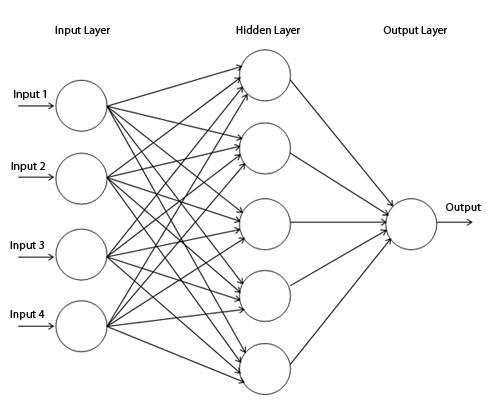
\includegraphics[scale=0.4]{mlp.jpeg}
\caption{Architektura MLP s jednou skrytou vrstvou}
\label{fig:mlp}
\end{center}
 \captionsetup{font={footnotesize,bf,it}}
  \caption*{zdroj: https://github.com/cazala/synaptic/wiki/Architect}
\end{figure}

 
 \subsection{Metody učení bez učitele}
  \subsubsection*{Hierarchical clustering}
  ENH
  \subsubsection*{K-means}

K-means je oblíbený algoritmus shlukové analýzy, kde počet shluků je předem určen parametrem $k$. Těchto $k$ shluků je definováno svými \textit{centroidy}, což jsou body ve stejném prostoru, jako vstupní vektory. Vstupní vektor náleží centroidu, kterému je nejblíže podle např. euklidovské vzdálenosti. Nalezení centroidů s optimálním shlukováním (minimální průměry shluků) je NP-tězký problém\cite{k-means-nphard}, proto se  používá následující heuristika\cite{k-means-algo}:

\begin{enumerate}
\item Náhodně vybereme $k$ centroidů,
\item  vstupní vektory přiřadíme nejbližším centroidům, čímž vznikne $k$ shluků,
\item těžiště každého shluku představuje centroid pro novou iteraci,
\item kroky 2-3 se stále opakují, dokud nedojde k ustálení.
\end{enumerate}


\section{SOM}\label{sec:som_teo}
Self organizing map (SOM), samoorganizující mapa, je umělá neuronová síť navržena Teuvo Kohonenem v 80. letech minulého století. Narozdíl od MLP se SOM skládá z jedné vrstvy speciálně uspořádaných neuronů. Dalším rozdílem je, že se učí bez učitele a to pomocí tzv. \textit{kompetitivní učení}.\cite{junkie}

\subsection{Struktura sítě}
SOM se typicky skládá z jedné vrstvy neuronů uspořádaných do pravidelné 2D mřížky\footnote{Je možné použít také 3D mřížky, nicméně v tomto textu budou použity výhradně 2D}. Topologie takové mřížky bývá zpravidla pravidelná a to hexagonání nebo pravoúhlá (obr. \ref{fig:top}). Složky vstupu jsou propojeny se všemi neurony.
Stejně jako dopředné sítě, SOM má ve spojích uložené váhy. Tuto skutečnost je však názornější zachycovat jako tzv.: \textit{prototypové vektory}, které jsou uloženy u jednotlivých neuronů. Každý prototypové vektor  má stejnou dimenzi jako je dimenze vstupních dat.

\begin{figure}
\centering
\begin{subfigure}{.5\textwidth}
  \centering
  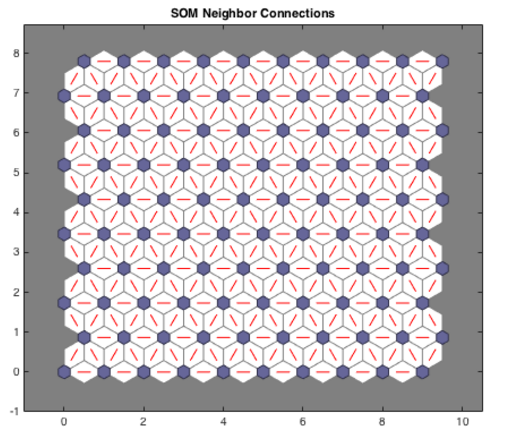
\includegraphics[width=.8\linewidth]{hex_top}
  \caption{Hexagonální topologie}
  \label{fig:sub1}
\end{subfigure}%
\begin{subfigure}{.5\textwidth}
  \centering
  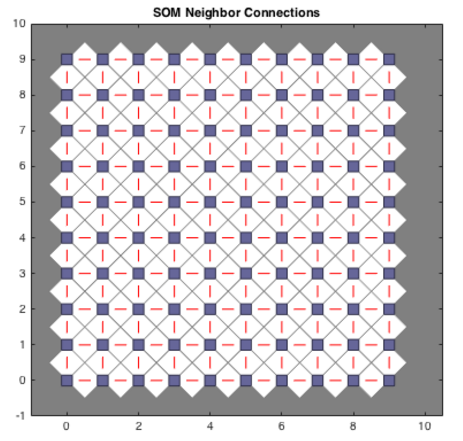
\includegraphics[width=.73\linewidth]{grid_top}
  \caption{Topologie organizovaná do pravoúhlé mřížky}
  \label{fig:grid_top}
\end{subfigure}
\caption{Modré značky představují neurony, zatímco červené spoje indikují sousedství.}
\label{fig:top}
\end{figure}

\subsection{Učení}

Jak již bylo zmíněno, samoorganizující se mapa se učí bez učitele a to kompetitivním učením. Základní myšlenka učícího algoritmu je následující: síti se opakovaně předkládají vstupy a váhové vektory neuronů jsou upravovány tak, aby více odpovídaly rozložení původního prostoru.
% je jich více, jeden z algoritmů
Konkrétně lze učení popsat pseudokódem:

\begin{enumerate}
\item Inicializace vektorů.
\item Jeden vstupní vektor je předložen síti.
\item Je nalezen neuron, který má se vstupem nejpodobnější váhový vektor. Pro tuto podobnost se dá použít např. euklidovská vzdálenost. Takový neuron se nazývá Best matching unit (BMU).
\item Váhový vektor každého neuronu je pak přiblížen vstupnímu vektoru. Velikost tohoto příblížení je určena \textit{neighborhood function} $\sigma(win, i, t)$ .
Závisí tedy na vzdálenosti neuronu od BMU, meřené v mřížce -- čím dále jsou neurony od sebe, tím je přiblížení slabší. Dále velikost těchto změn slábnou s každou iterací učení. Celý vztah pro úpravu váhového vektoru W neuronu i je určen vztahem \ref{eq:1}.


\item Znovu body 2 - 5 po N iterací.
\end{enumerate}

\begin{equation} \label{eq:1}
    \mathcal{W}_i(t+1) = \mathcal{W}_i(t) + \alpha \sigma(win, i, t)(\mathcal{X}(t) - \mathcal{W}_i(t))    
\end{equation}

Kde:\\
\hspace*{3em}
\begin{tabular}{rl}
    $\mathcal{X}(t)$:& vstupní vektor \\
    $\mathcal{W}_i(t)$:& váhový vektor neuronu $i$ \\
    $\alpha$:& \textit{learning rate} -- zvolená konstanta, může být i funkcí epochy \\
\end{tabular}


\subsection{Vlastnosti}
SOM, stejně jako mnoho dalších dataminingových metod, předpokládá, že příslušnost tříd je definovaná podobností atributů.

Dále je chování samoorganizujících map ovlivněno počtem neuronů -- bylo ukázáno, že samoroganizující mapy s relativně malým počtem neuronů (oproti velikosti datasetu) se chovají podobně jako metoda K-means\cite{needed}. Prototypové vektory pak  představují středy shluků v původním prostoru.

Naopak pro sítě s počtem neuronů srovnatelným s počtem vstupních dat, SOM učením vytváří diskrétní reprezentaci vstupního prostoru -- \textit{mapu}, ktera zachovává topologické vlastnosti prostoru, založené na sousednosti (co bylo blízko ve vstupním prostoru bude blízko i na mapě).
% neighboorhood function



\subsection{Využití}

Jelikož se vlastnosti samoorganizujících map různí podle počtu použitých neuronů, využití se liší taktéž podle tohoto parametru.

SOM s malým počtem neuronů je možné využít tam, kde je možné použít K-means. (\dots TODO: výhody, nevýhody, rozdíly)


Naopak samoorganizující mapy s velkým\footnote{Velký počet v tomto smyslu představuje řádově srovnatelný s počtem vstupních vektorů.} počtem neuronů se používají převážně jako nástroj pro redukci dimenzionality.  Toho lze využít v transformaci dat při procesu KDD (\ref{subsec:transformace}), podobně, jako ostatní metody s tímto účelem\cite{som_dim_red}. Kterýkoliv vektor ze vstupního prostoru je namapován na pozici v mřížce -- ta je určena pozicí neuronu, který se aktivuje pro příslušný vstupní vektor, jinými slovy je pro něj BMU.


Dále je možné zkoumat naučenou \textit{mapu}. Tato mapa je určena prototypovými vektory neuronů, které mohou sloužit jako vstupní prostor pro další shlukovou analýzu\cite{som_clustering}. Dále je mapa, díky své nízké dimenzionalitě, vhodná pro vizualizace a 
\textit{explorační analýzu}\footnote{Explorační analýza představuje metody pro průzkum dat a hledání hypotéz.}, což je také nejrozšířenější použití samoorganizujích map.



\subsubsection*{Vizualizace map}
Vizualizace je mocný nástroj pro extrakci znalostí a hypotéz z dat, převážně protože do procesu zahrnuje lidské vnímání, zkušenosti a kreativitu, které jsou při takové činnosti klíčové\cite{visual}. Bohužel tyto lidské schopnosti, stejně tak jako možnosti vizualizace, jsou značně omezené, pokud jsou data vysoce dimenzionální. Jak již ale bylo zmíněno, samoorganizující mapy poskytují dvou-dimenzionální reprezentaci dat, kterou je možné snadno vizualizovat.

Jedním způsobem jak zobrazovat natrénovanou mapu, je zobrazit vstupní data spolu s pozicemi neuronů. Tímto přístupem ovšem získáme náhled pouze na dvě dimenze. Na obrázku \ref{fig:plotsompos} je příklad takového vykreslení pro dvou-dimenzionální problém. Zelené body představují vstupní vektory, modré značky jsou neurony a červené spoje znázorňují sousedství mezi neurony. Neurony jsou na mapě vykresleny na místě podle svého prototypového vektoru, který je stejně jako vstupní prostor, dvou-dimenzionální.



\begin{figure}[htbp]
\begin{center}
	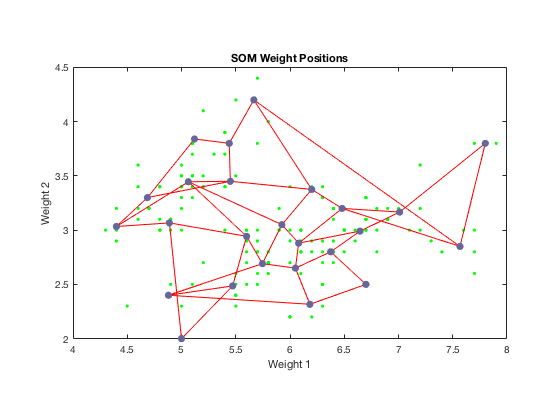
\includegraphics[scale=0.5]{iris_plotsompos.png}
\caption{Zobrazení natrénované SOM s neurony uspořádanými do pravoúhlé mřížky 5x5 pro náhodný dvoudimenzionální problém.}
\label{fig:plotsompos}
\end{center}
\end{figure}


Další možností je vizualizovat mřížku spolu s dalšími informacemi (třídy), které mohou být již obsaženy ve vstupních vektorech. Pro každý vstupní vektor se spočítá jeho BMU na natrénované SOM. Takovému neuronu se pak přiřadí třída patřící onomu vstupnímu vektoru. Po aplikaci všech vstupních vektorů nastane pro každý neuron jedna z následujících možností:

\begin{itemize}
\item neuron má přiřazenu třídu $k$ -- vykreslí se s barvou přiřazené třídě $k$,
\item  neuron má přiřazené dvě a více tříd -- vykreslí se s černou barvou.
\end{itemize}
 
Velikost každého neuronu pak roste s počtem přiřazených tříd, přičemž neuron bez přiřazené třídy má nulovou velikost a na mapě se vůbec nebjeví. Takové vykreslení se nazývá \textit{sémantická mapa}, jejíž příklad je na obr. \ref{fig:semanticmap}.


\begin{figure}[htbp]
\begin{center}
	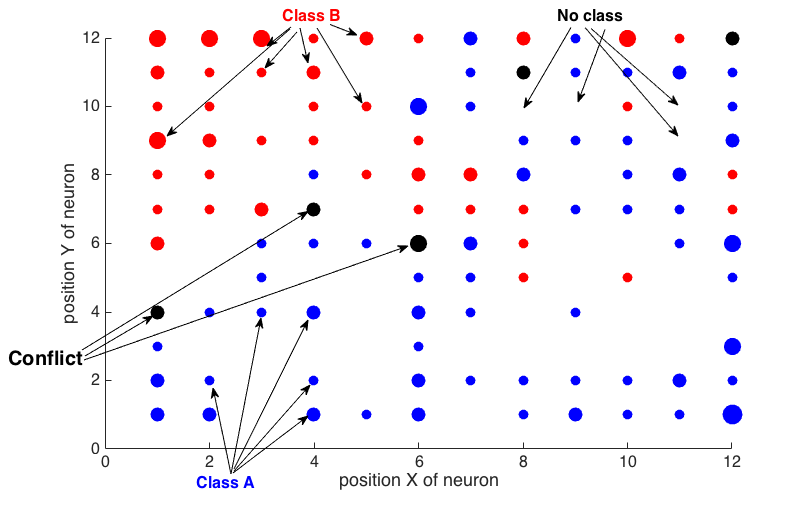
\includegraphics[scale=0.4]{semantic_map.png}
\caption{Příklad sémantické mapy pro dvě třídy.}
\label{fig:semanticmap}
\end{center}
\end{figure}


ENH: další možnosti

% http://stackoverflow.com/questions/18233994/interpreting-a-self-organizing-map


\section{CRSOM}\label{sec:crsom_teo}
\textit{Context-relevant self organizing map, Samoorganizující mapa se zahrnutým sémantickým kontextem (CRSOM)} je umělá neuronová síť navržena Pitoyo Hartonem. Narozdíl od kasické SOM se CRSOM učí s učitelem, z čehož vyplývá, že k učení je nutné znát dvojice vstupní a výstupní vektor. Právě výstupní vektory určují tzv. \textit{kontext učení}, což mohou být například třídy vstupních vektorů.

\subsection{Struktura sítě}
CRSOM se skládá ze tří vrstev neuronů. Prostřední (skrytá) vrstva je organizovaná do 2D mřížky neuronů, tzn. stejně jako u klasické samoorganizující mapy.
 Oproti SOM má CRSOM ještě jednu vrstu navíc -- výstupní (\textit{kontextovou}).  Každý neuron výstupní vrstvy je propojen s každým neuronem ve skryté SOM vrstvě (viz obr. \ref{fig:crsom_structure}). 
 

\begin{figure}[htbp]
\begin{center}
	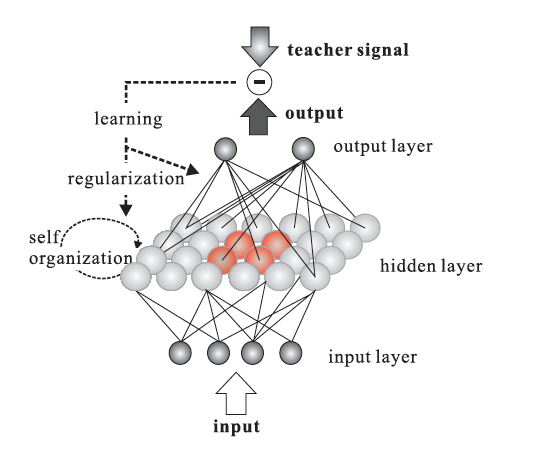
\includegraphics[scale=0.6]{crsom_structure}
\caption{TODO: zdroj}
\label{fig:crsom_structure}
\end{center}
\end{figure}
 
 

\subsubsection*{Výstup sítě}
Výstup celé sítě je složená funkce vstupního vektoru. 
Jínými slovy první z vrstev aplikuje svou funkci na vstupní vektor a každá další vrstva aplikuje svou funkci na výstup neuronů z předchozí vrstvy. Tento přístup je stejný jako u MLP. V následujícím odstavci budou probrány jednotlivé funkce vrstev a jejich význam.

\subsubsection*{Skrytá vrstva}
První funkce, jejíž vstupem je konkrétní vstupní vektor, je $ \mathcal{O}_h^i(t) $. Tato funkce představuje míru aktivace i-tého neuronu ve skryté vrstvě. $ \mathcal{O}_h^i(t) $ se skládá ze dvou multiplikativních členů \ref{eq:2}.

\begin{equation} \label{eq:2}
    \mathcal{O}_h^i(t) = e^{-\mathcal{I}_i^h(t)} \sigma(win, i, t)
\end{equation}


První z členů představuje vztah aktivace neuronu $i$  a podobnosti vstupního a příslušného váhového vektoru -- \textit{prostorovou aktivaci}. Tato funkce (\ref{eq:3}) zobrazuje vzdálenost dvou vektorů do intervalu $(0;1]$.


\vspace{\baselineskip}
\noindent
\begin{minipage}[c]{\textwidth }
\begin{equation} \label{eq:3}
    \mathcal{I}_h^i(t) = \|\mathcal{X}(t)-\mathcal{W}_i(t)\|^2   
\end{equation}

Kde:\\
\hspace*{3em}
\begin{tabular}{rl}
    $\mathcal{X}(t)$:& vstupní vektor \\
    $\mathcal{W}_i(t)$:& váhový vektor neuronu $i$ \\
\end{tabular}
\end{minipage} 
\vspace{\baselineskip}
\noindent

 

Druhý člen představuje \textit{topologickou restrikci} v mapě neuronů (\ref{eq:4}). Jinými slovy jde o aktivování neuronů v závislosti na pozici v mřížce. Čím blíže je neuron k BMU, tím je tato aktivace vyšší, zároveň tato aktivace klesá s časem, které je zajištěné funkcí $s(t)$ popsanou vztahem \ref{eq:5}.  
V této praci byly parametry $s_0$ a $s_{end}$ nastaveny na $200$ a $0.01$, stejně tak, jak je navrženo a empiricky otestováno v originální publikaci \cite{hartono14}.


\vspace{\baselineskip}
\noindent
\begin{minipage}[c]{\textwidth }

\begin{equation} \label{eq:4}
    \sigma(win, i, t)=e^-\frac{dist(win, i)}{s(t)}  
\end{equation}

\begin{equation} \label{eq:5}
    {s(t)=s_0(\frac{s_{end}}{s_0})^\frac{t}{t_{end}}}  
\end{equation}

Kde:\\
\hspace*{3em}
\begin{tabular}{rl}
    $dist(win, i)$:& vzdálenost BMU a neuronu $i$, měřeno na mřížce \\
    $s_0$, $s_{end}$ :& $200$, $0.01$ \\
     $t$, $t_{end}$:& současná epocha, celkový počet epoch \\
\end{tabular}
\end{minipage} 
\vspace{\baselineskip}
\noindent

Na obrázku \ref{fig:top_restr} jsou zobrazeny tři mřížky neuronů. Každý z obrázků představuje výstup skryté vrstvy pro stejný vstup, ale v různých fázích učení (v různých epochách). Každá diskrétní pozice $(x, y)$ tedy představuje jeden neuron a velikost značky na pozici $(x, y)$ představuje relativní míru aktivace s tím, že BMU je v těchto případech na pozici  $(7, 7)$.

Grafy se liší pouze fází účení -- tedy epochou. V prvním případě je stav aktivace neuronů zobrazen na počátku učení, konkrétně v $8.$ epoše z celkových $50$. Graf dokumentuje skutečnost, že v této fázi jsou do formování mapy zahrnuty velkou měrou všechny neurony na mapě. V dalších dvou případech, které zobrazují stav ve $20.$ resp. $30.$ epoše, je rozpoznatelné zmenšující se okolí BMU, které je řízeno funkcí $s(t)$.


Oproti tomu na obr \ref{fig:sigma} je zobrazena závislost míry aktivace pro celý průběh učení pro fixní vzdálenost neuronů. V prvním grafu je vykreslena funkce $\sigma$ pro neurony vzdálené $1$, což se dá interpretovat jako míru topologické aktivace pro nejbližší neuron k BMU.
Na zbylých grafech jsou zobrazeny průběhy pro větší vzdálenost od BMU -- konkrétně $7$ a $25$. Z grafů je zřetelné, že vzdálené neurony od BMU se do formování mapy výrazněji zahrnují jen v počátečních fázích učení. Zahnutí neuronů pak strmě klesá a např. neurony vzdálené 25 se do formování mapy po 40. epoše zahrnují jen zanedbatelnou měrou.

\begin{figure}[htp]

\centering
\hspace*{-1cm}
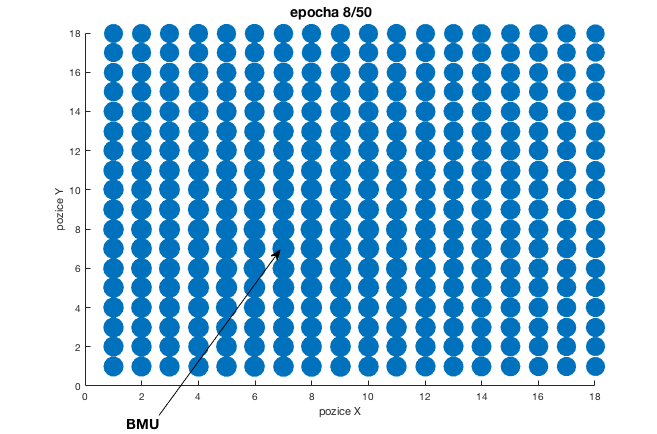
\includegraphics[width=.33\textwidth]{top_restr_8.png}
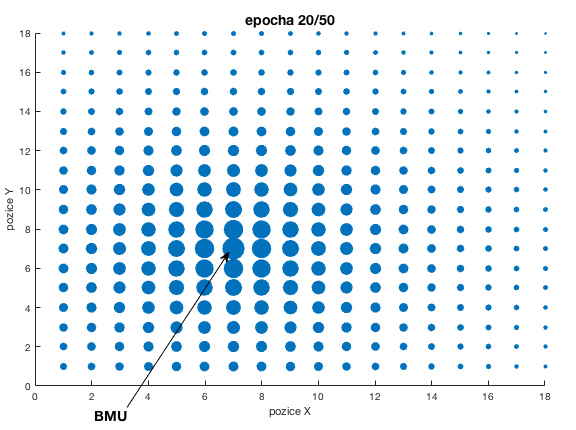
\includegraphics[width=.33\textwidth]{top_restr_20.png}
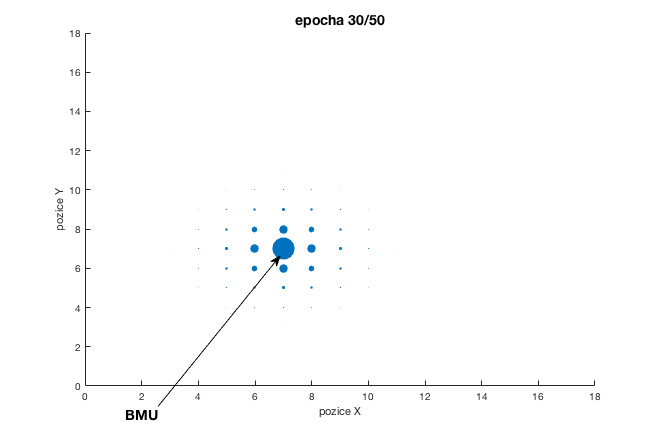
\includegraphics[width=.33\textwidth]{top_restr_30.png}
\hspace*{-1cm}
\caption{Příklad aktivace neuronů pro různé fáze učení.}
\label{fig:top_restr}

\end{figure}


\begin{figure}[htp]

\centering

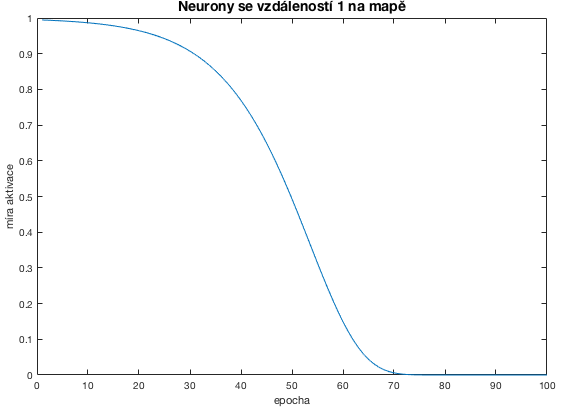
\includegraphics[width=.32\textwidth]{sigma_1.png}
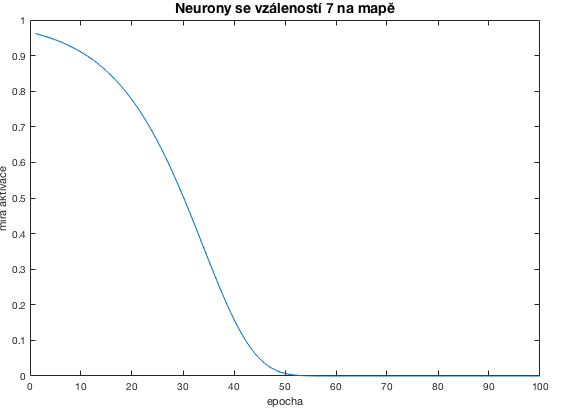
\includegraphics[width=.32\textwidth]{sigma_7.png}
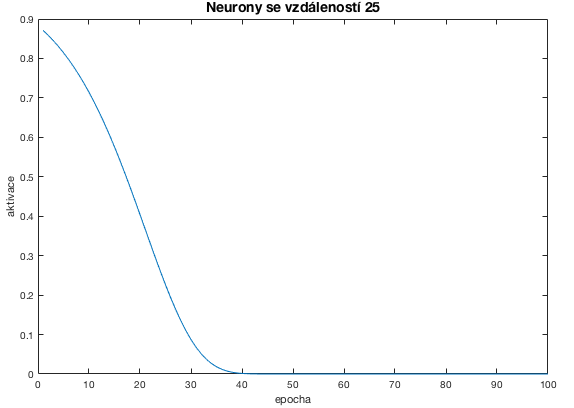
\includegraphics[width=.32\textwidth]{sigma_25.png}
\caption{Míra aktivace po celé učení pro různé vzdálenosti od BMU}
\label{fig:sigma}

\end{figure}


\subsubsection*{Výstupní vrstva}
Výstup neuronů skryté vrstvy slouží jako vstup do výstupní vrstvy sítě. Výstupní vrstva funguje jako jedna běžná vrstva MLP. Tedy výstup neuronu  $k$ ve výstupní vrstvě je dán funkcí $\mathcal{O}_k(t)$ (\ref{eq:6}).

\vspace{\baselineskip}
\noindent
\begin{minipage}[c]{\textwidth }

\begin{equation*}
   \mathcal{I}_k(t) = \sum\limits_i{v_{ik}(t)\mathcal{O}_i^h - \theta_k(t)}  
\end{equation*}

\begin{equation} \label{eq:6}
   \mathcal{O}_k(t) = f(\mathcal{I}_k(t))
\end{equation}


Kde:\\
\hspace*{3em}
\begin{tabular}{rl}
    $\theta_k(t)$:& bias pro neuron $k$ \\
    $f(x) $ :& sigmoida, $\frac{1}{1+e^{-x}}$ \\

\end{tabular}
\end{minipage} 
\vspace{\baselineskip}
\noindent

\subsection{Učení}
Protože se CRSOM učí s učitelem, ke každému vstupnímu vektoru máme požadovaný výstupní vektor. Lze zavést funci $E(t)$, která bude sloužit jako chybová funkce.

\vspace{\baselineskip}
\noindent
\begin{minipage}[c]{\textwidth }

\begin{equation} \label{eq:e}
   E(t)=\frac{1}{2}\sum\limits_k{(\mathcal{O}_k(t)-\mathcal{T}_k(t))^2}  
\end{equation}


Kde:\\
\hspace*{3em}
\begin{tabular}{rl}
    $\mathcal{O}_k(t)$:& výstup neuronu $k$ \\
    $\mathcal{T}_k(t) $ :& požadovaný výstup pro neuron $k$ \\

\end{tabular}
\end{minipage} 
\vspace{\baselineskip}
\noindent


Funkce $E(t)$ představuje chybu pro vstupní vektor a nastavení sítě v podobě vah. Jedním ze způsobů jak optimalizovat takovou funkci je \textit{metoda nejstrmějšího sestupu}, tedy pomocí gradientu funkce $E(t)$. Změny ve výstupní vrstvě -- tedy váhových vektorů $v_{ik}$ a biasu $ \theta_k$ -- se řídí podle následujících vztahů:

\vspace{\baselineskip}
\noindent
\begin{minipage}[c]{\textwidth }

\begin{equation*}
   v_{ik}(t+1)=v_ik(t) - \eta_1\frac{\partial{E(t)}}{\partial{v_{ik}(t)}} =  v_{ik}(t) - \eta_1\delta_k(t)\mathcal{O}_h^i(t) 
\end{equation*}

\begin{equation*}
   \theta_k(t+1)=\theta_k(t) - \eta_1\frac{\partial{E(t)}}{\partial{\theta(t)}} = \theta(t)  + \eta_1\delta_k(t)
\end{equation*}

\begin{equation*}
   \delta_k(t) = (O_k(t) - T_k(t))O_k(t)(1-O_k(t)) 
\end{equation*}

Kde:\\
\hspace*{3em}
\begin{tabular}{rl}
    $\eta_1$:& \textit{learning rate} pro výstupní vrstvu \\
\end{tabular}
\end{minipage} 
\vspace{\baselineskip}
\noindent

    

Stejným spůsobem se pak upravují i váhové vektory neuronů ve skryté vrstvě \ref{eq:adj}
  
  \vspace{\baselineskip}
\noindent
  \begin{minipage}[c]{\textwidth }

\begin{equation*}
   \mathcal{W}_i(t+1)=W_i(t) -  \eta_2\frac{\partial{E(t)}}{\partial{W_i(t)}} 
\end{equation*}

\begin{equation*}
   \delta_i^h(t)=-e^{-I_i^h(t)}(\sum\limits_k{\delta_k(t)v_{ik}(t)})
\end{equation*}

\begin{equation}\label{eq:adj}
   \mathcal{W}_i(t+1)=\mathcal{W}_i(t) -  \eta_2\delta_i^h(t)\sigma(win, i, t)(\mathcal{X}(t) - \mathcal{W}_i(t))
\end{equation}

Kde:\\
\hspace*{3em}
\begin{tabular}{rl}
    $\eta_2$:& \textit{learning rate} pro skrytou vrstvu \\
        $\mathcal{X}(t)$:& vstupní vektor \\
            $\mathcal{W}_i(t)$:& prototypový vektor neuronu $i$ \\
\end{tabular}
\end{minipage} 
\vspace{\baselineskip}
\noindent
 

\subsection{Srovnání se SOM }
\subsubsection*{Rozdíl ve formování SOM a CRSOM}
Narozdíl od vztahu, který popisuje úpravy prototypových vektorů v sítích typů SOM (\ref{eq:1}), se v úpravách prototypových vektorů CRSOM (\ref{eq:adj}) navíc vyskytuje člen $\delta_i^h(t)$.

Tento člen slouží jako \textit{regulační signál}, který je určen velikostí chyby na výstupu. Slouží tak jako zpětná vazba z kontextové sítě, která řídí formování skryté vrstvy podle zadaného kontextu.

Pouze v případě $ \delta_i^h(t) > 0 $, je neuron $i$ přiblížen ke vstupnímu vektoru. V případě $ \delta_i^h(t) < 0 $ je naopak oddálen. Z toho vyplývá, že ke vstupnímu vektoru jsou přiblíženy pouze prototypové vektory neuronů, které přispívají ke snížení chyby, ostatní jsou naopak pokutovány oddálením. To má za důsledek rozdílné chování oproti SOM, kde mapa je formována pouze na základě vstupního prostoru, zatímco u CRSOM je mapa formována na základě vstupního prostoru a dodaného semantického kontextu. 

Formování mapy CRSOM je ukázáno na obr. \ref{fig:cr}. Vstupní data tvoří dataset Iris\footnote{Známý dataset dostupný na adrese: https://archive.ics.uci.edu/ml/datasets/Iris} omezený na dvě dimenze \ref{fig:iris2d}. Toto omezení umožní vizualizovat mapu a vstupní data na jednom grafu bez ztráty informace. Ze série obrázků (\ref{fig:cr}) je vidět, že formování respektuje sémantický kontext, kterým jsou v tomto případě jednotlivé třídy datasetu Iris. Mapa vytváří shluky, které odpovídají rozložení tříd ve vstupním prostoru.




\begin{figure}[htp]    
    \centering
    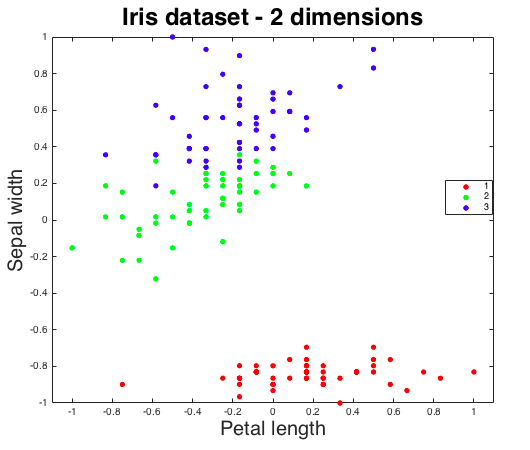
\includegraphics[width=0.6\textwidth]{feature_space_with_classes.png}
    \caption{Dataset Iris omezený na dvě dimenze.}
    \label{fig:iris2d}
\end{figure}


V případě, že $ \delta_i^h(t)$ je zafixováno na $1$, CRSOM simuluje chování SOM: prototypové vektory jsou ke vstupnímu vektoru přiblíženy vždy, bez ohledu na sémantický kontext a výstup sítě. Simulace klasické samoorganizující mapy pomocí CRSOM je doložen na obr. \ref{fig:delta_1}.


\begin{figure}[htp]
    \centering
    
    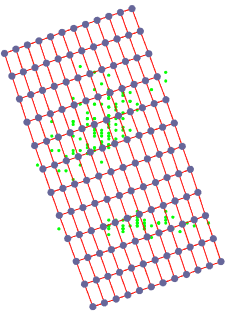
\includegraphics[width=.32\textwidth]{cr1.png}
    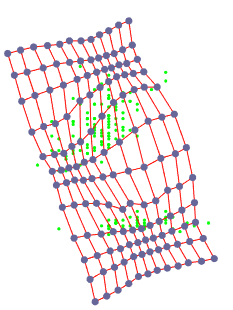
\includegraphics[width=.32\textwidth]{cr2.png}
    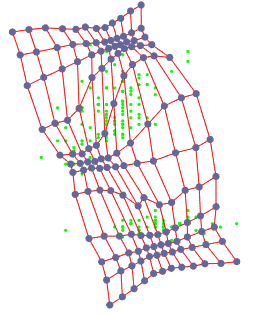
\includegraphics[width=.32\textwidth]{cr3.png}
    \caption{Mapa CRSOM se formuje s ohledem na sémantický kontext.}
    \label{fig:cr}
\end{figure}

\begin{figure}[htp]
    \centering
    
    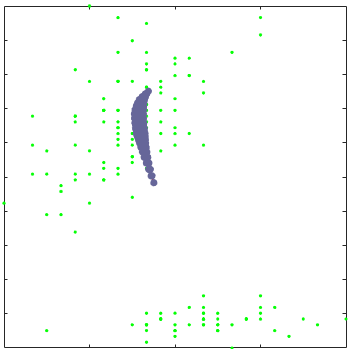
\includegraphics[width=.32\textwidth]{s1.png}
    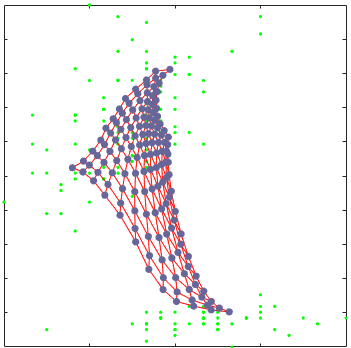
\includegraphics[width=.32\textwidth]{s2.png}
    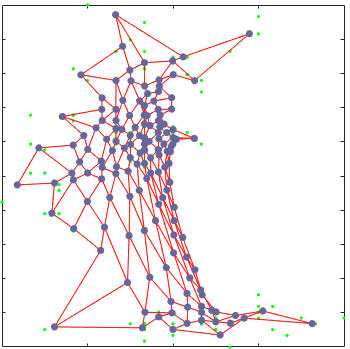
\includegraphics[width=.32\textwidth]{s3.png}
    \caption{CRSOM se chová stejně jako SOM pro zafixované $ \delta_i^h(t) = 1 $ }
    \label{fig:delta_1}
\end{figure}


\subsubsection*{Rozdíl v interpretaci map SOM a CRSOM}
Samoorganizující mapy jsou schopné vysoce dimenzionální prostor mapovat do 2D a zachovat při tom některé topologické vlastnosti vstupního prostoru. Pokud máme k datům nějaký kontext (třídy) a chceme je nějakým způsobem využít pro formování mapy, není jiná možnost, než využít třídy jako další atributy. Naopak CRSOM s těmito informacemi zachází explicitně a pomocí těchto tříd prostřednictvím regulačního signálu řídí formování mapy podle zadaného kontextu. SOM je schopný vizualizovat strukturu vstupního prostoru, zatímco CRSOM je schopná vizualizovat strukturu problému\cite{hartono14}.



\subsection{Vlastnosti a využití}

	CRSOM naučená na konkrétní sémantický kontext může být využita jako klasifikátor tohoto kontextu pro nová data. V takovém případě mapa, která je definovaná skrytou SOM vrstou, představuje vedlejší produkt takového učení. Tato mapa nám dává intuitivní pochopení výkonnosti takového klasifikátoru.

Kromě toho je možné považovat mapu jako cílový produkt učení. Vzniklá mapa pak může sloužit k vizualizacím klasifikačního problému pro daný sémantický kontext. Dále je možné z mapy extrahovat znalosti a strukturu v podobě vytvořených shluků, stejně jako u SOM s tím rozdílem, že výsledek CRSOM respektuje při formování sémantiku a je možné z něho extrahovat rozdílné znalosti \cite{lms}.

% -------------------------------------- Návrh a implementace ---------------------------------------------------------------------------------------------------------------------------------------------------------------
\chapter{Návrh a implementace}
V této kapitole jsou rozebrány nutné kroky pro použití vybraných metod. Zaprvé bylo nutné zajistit implementace oněch metod a zadruhé navrhnout a implementovat platformu pro experimentování s metodami. Pro implementaci metod bylo zvoleno prostředí \textit{Matlab}. Pro práci s experimenty byly zvoleny \textit{Ruby}, \textit{MongoDb}, \textit{Git} a \textit{MetaCentrum}. V této kapitole jsou popsány důvody pro zvolení právě těchto technologií a nástrojů, spolu s popisem jejich využití a vzájemného fungování. 


\section{SOM}\label{sec:som_impl}
Hotová implementace samoorganizujících map je dostupná pro mnoho platforem, Matlab byl zvolen zejména kvůli existenci speciálního toolboxu\footnote{Toolbox je označení pro rozšíření Matlabu a jeho IDE} pro neuronové sítě. Kromě toho Matlab nabízí širokou škálu vykreslování a jednoduchou manipulaci s maticemi. Je třeba také zmínit, že ČVUT vlastní licence na Matlab a příslušné toolboxy pro akademické použití, čímž odpadá finanční stránka rozhodování, která by v neakademickém použití hrála významnou roli.
Pro samoorganizující mapy se v Matlabu používá funkce \texttt{selforgmap}\footnote{Dokumentace je dostupná na http://www.mathworks.com/help/nnet/ref/selforgmap.html}. Kód pro natrénování samoorganizující mapy o velikosti 10x10 stačí kód zobrazen v ukázce \ref{somcode}.

\begin{listing}
    \begin{minted}[linenos=true,bgcolor=bg]{matlab}
        som = selforgmap([10 10])
        trained_som = train(som, inputs)
    \end{minted} 
    \caption{Vytvoření samoorganizující mapy v prostředí Matlab.} 
    \label{somcode}
\end{listing}

\section{CRSOM}\label{sec:crsom_impl}


Implementace CRSOM byla mnohem náročnější. Jedním z důvodů bylo to, že v době implementace bylo k dispozici pouze analytické vyjádření fungování sítě, bez jakékoliv vzorové implementace.
Správnost sítě tak bylo možné verifikovat pouze na základě výstupů z experimentů provedených Hartonem na známých datových sadách\cite{hartono14}.

Další překážkou bylo, že prováděné experimenty byly spouštěny pro $30 000$ epoch, což by znamenalo několik dní výpočtů pro první naivní implementace.
	
Postup pro implementaci sítě tak, jak byla navržena Hartonem, byl inspirován přístupem \textit{\uv{Make it work, make it right, make it fast}}\cite{makeit}. 
Tento přístup logicky prioritizuje vývoj software: jako první by měla být zaručena korektní implementace. Až poté je možné implementaci vylepšovat ve směrech designu, robustnosti a výkonu. Pro zachování správnosti software je nutné zavést regresní testování, které zaručí pokračující korektnost i po změnách v rámci \uv{Make it right} a \uv{make it fast}.

\subsection{Make it work}
 Jak bylo zmíněno, první naivní implementace sítě není možné verifikovat oproti Hartonovým experimentům, nadruhou stranu je z definice sítě a z dostupných publikací (např.: \cite{hartono14}) zřejmé, jak se bude mapa formovat pro jednoduché příklady. Takovým jednoduchým příkladem je například dobře známý dataset Iris. Tento dataset byl navíc omezen na dvě dimenze, což poskytuje možnost vizualizovat neurony, určené prototypovými vektory, spolu se vstupními daty v jednom vykreslení. Vizualizace formování se ukázala, jako velmi platná pro pochopení a ladění fungování sítě. Kromě zobrazování neuronů na mapě spolu se vstupními daty, byly ukládány a zanášeny do grafů další hodnoty významné pro průběh učení. Mezi takové hodnoty patří například hodnota funkce $E(t)$, průměrné výstupy neuronů ze skryté vrstvy, průměrná topologická restrikce a další.
 
Další překážkou byla vysoká citlivost metody na nastavení parametrů učení\cite{hartono14}. Slabé výsledky tak nemusí vždy znamenat chybu v implementaci, nýbrž například nevhodné nastavení učících parametrů. Tomuto problému bylo čeleno pomocí prohledávání prostoru parametrů a kontrolování všech výsledků, alespoň z počátku verifikace.
Pomocí těchto přístupů se podařilo naimplementovat CRSOM, která dávala srovnatelné výsledky na stejných datasetech podle originálních publikací \cite{hartono14}. (ENH: doložení obrázky)

\subsection{Make it right and make it fast}

První verze sítě byla sice funkční, trpěla ale několika prohřešky jak z výkonového hlediska, tak z designového. Ještě před jakýmikoliv úpravami bylo nutné vytvořit sadu regresních testů, které budou zajišťovat stálou správnost sítě. Toho bylo docíleno odebráním všech nedeterministických nastavení a uložení stavu sítě po několika epochách učení \textit{(expected net)} pro daný testovací dataset.  Regresní testování upravené sítě pak spočívalo ve spuštění učení se stejným nastavením a pro stejný dataset jako pro síť \textit{expected net}. Za předpokladu deterministického učení, naučená síť musí mít stejné hodnoty prototypových vektorů jako \textit{expected net}.

Výkon sítě se měřil pomocí učení na datasetu, který byl výrazně větší, než dataset určený pro testování. K určení problémových míst implemetace, z hlediska výkonu, byl výhradně používán Matlab profiler\footnote{http://www.mathworks.com/help/matlab/matlab\_prog/profiling-for-improving-performance.html}, který je vestavěný do IDE. Zlepšování sítě bylo provádělo iteračně, od první naivní implementace se učení zrychlilo více než $15$x, výsledky a měření samotné je popsáno v \ref{measure}. Nejvýraznější pokroky ve výkonu byly dosaženy následujícími upravami:





\subsubsection*{Vektorizace}
Matlab je optimalizován pro práci s vektory a maticemi, tím pádem kód, který je \textit{vektorizovaný}(ukázka \ref{vector-code}) je mnohem rychlejší\cite{vector}, než ten vyvořený pomocí \textit{smyček}(ukázka \ref{for-code}).


\begin{listing}
\begin{minted}[linenos=true,bgcolor=bg]{matlab}
delta_h = zeros(NEURONS,1);
for i = 1:NEURONS
    s = sum(delta_k.* cn.IW{1}(i));
    delta_h(i) =  first_part(i) * s;
end
\end{minted} 
\caption{Kód zapsaný pomocí for smyčky.} 
\label{for-code}
\end{listing}

\begin{listing}
\begin{minted}[linenos=true,bgcolor=bg]{matlab}
s = sum((repmat(delta_k', NEURONS, 1).*(cn.IW{1}'))')';
delta_h = first_part .* s;
\end{minted} 
\caption{Vektorizovaný kód.} 
\label{vector-code}
\end{listing}







\subsubsection*{Prealokace}
Pokud je předem známá velikost požadované matice, je vždy rychlejší naalokovat celkový kus paměti dopředu, než požadovanou iterativně navyšovat\cite{preallocate}.




\subsubsection*{Funkce adapt}
První verze používaly oddělenou kontextovou síť vytvořenou pomocí funkce \texttt{network}. Tato síť se pak doučovala pomocí funkce \texttt{adapt}. Tento přístup však není vhodný pro cyklické opakování, zejména kvůli znovuvytváření všech obecných struktur s informacemi o učení. Pozdější verze sítě již tento přístup vůbec nevyužívaly.


\subsubsection{Měření výkonu}\label{measure}
\ref{my-measure}
dataset
tic-toc
stroj
kolikrát

\begin{table}[]
\centering
\caption{Délka učení pro různé verze implementace}
\label{my-measurel}
    \begin{tabular}{|l|c|c|}
        \hline
        Verze                         & \multicolumn{1}{l|}{průměrný čas} & \multicolumn{1}{l|}{odchylka} \\ \hline
        bench0                        & 10000s                                           & 10s                                    \\ \hline
        bench2                        & 10000s                                           & 10s                                    \\ \hline
        bench3                        & 10000s                                          & 10s                                    \\ \hline
        \textbf{bench4}               & \textbf{2087s}                                    & \textbf{15s}                           \\ \hline
    \end{tabular}
\end{table}


\subsection{Konečný design}
TODO

\subsubsection{Publikování sítě}
TODO

\section{Implementace experimentů}

Celý proces implementace a experimentování na cílových datech přineslo několik problémů, kterým bylo nutné čelit. 
Použitá data byla dostupná přes veřejné API a velikost jednoho surového záznamu byl poměrně veliký (stovky Kb).
Proces implementace si vynutil současnou existenci několika různých verzí sítě s rozdílným nastavení  parametrů. Z důvodu dlouhé prodlevy mezi změnou a výsledkem bylo nutné efektivně zaznamenávat důvod konkrétních změn a jejich kontext.
Samotné experimenty pak vyžadovaly časté spouštění trénování pro různé datové sady a různé nastavení parametrů učení. Výsledky experimentů pak bylo nutné jednoduše vyhodnocovat, třídit a ukládat. To vše ohledem na vysokou výpočetní a prostorovou náročnost metody a nemožností paralelizace na osobním stroji s jednou Matlab licencí. 


\subsection{Tvorba datasetů}

Je třeba zmínit, že všechny vytvořené datové sady pocházely z jednoho zdroje. Z důvodu poměrně objemných záznamů bylo vhodné tato data cachovat do lokální databáze. Pro tento účel byla zvolena MongoDb databáze. Samotné stahování dat z API a generování datasetů bylo docíleno skripty v programovacím jazyce Ruby. V této sekci budou představeny tyto klíčové technologie spolu s důvodněním jejich výběru. Spolupráci technologií při stahování dat z API následné generování datasetů je pak zobrazena na obr. \ref{fig:down}.

\begin{figure}[htbp]
\begin{center}
	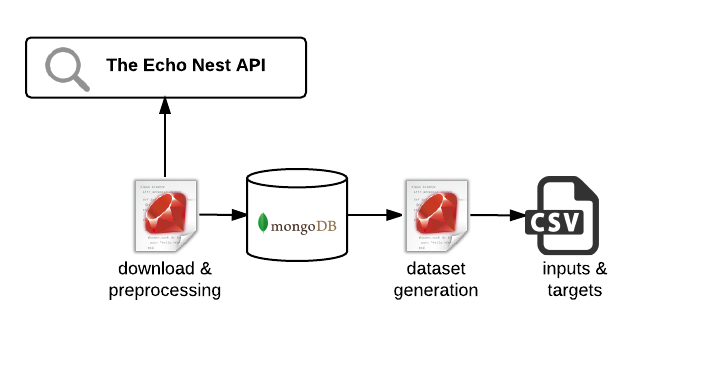
\includegraphics[scale=1]{download_generate.png}
\caption{Stahování dat z API a generování datasetů}
\label{fig:down}
\end{center}
\end{figure}

\subsubsection*{MongoDb}
MongoDb je dokumentově orientovaná databáze, tedy patří mezi tzv. \textit{NoSQL} databáze. MongoDB umožňuje ukládat data bez dopředu známého schématu, což byl nejvýznamější důvod pro použití právě takové databáze.

Data v MongoDb jsou interně uložena a navenek prezentována ve formátu BSON, což je specifikace a knihovna pro převod JSONu do binární podoby. Data, která poskytuje The Echo Nest prostřednictvím webového API, jsou taktéž ve formátu JSON, Tato skutečnost dělá dokumentovou databázi mnohem lepším kandidátem, než by tomu byly tradiční relační databáze. Navíc, pro využítí databáze jako lokální cache, jsou nepotřebné další vlastnosti, které nabízejí relační databáze, jako jsou transakční zpracování, integritní omezení a další.

\subsubsection*{Ruby}
Pro ukládání dat do MongoDB a následné generování datasetů ve formátu csv by zvolen jazyk Ruby. Ruby je interpretovaný skriptovací jazyk, který vznikl v roce 1995 v Japonsku.
Jazyk Ruby byl zvolen pro svou jednoduchou syntax, možnost krátkého zápisu kódu a širokou dostupnost \textit{gemů}\footnote{Gem je označení pro balíček kódu v jazyce Ruby}. Příkladem použitého gemu je Mongoid, který slouží jako ODM\footnote{Object-Document-Mapper -- mapování mezi dokumenty v databázi a ruby objekty.} framework pro databázi MongoDb.
Jednou ze slabých stránek jazyka Ruby je výkon \cite{ruby_performance}, alespoň ve srovnání s kompilovanými jazyky jako je např \texttt{C++}. Tato nevýhoda je ovšem pro toto konkrétní použítí nevýznamná, naopak snadný zápis kódu a dostupnost gemů znamená obrovskou časovou úsporu a snadnou modifikaci kódu.


\subsection{Framework na experimenty}
Jak již bylo zmíněno, velké množství experimetů pro různé verze kódu a konfigurace metod přinesly spousty požadavků. Mezi požadavky mimo jiné patřilo napřiklad jednoduché nasazování kódu, logování, paralelní pouštění experimentů, uchovávání výsledků a další. Pro naplnění těchto požadavků byly zvoleny dvě hlavní technologie: výpočetní centrum \textit{MetaCentrum} a verzovací nástroj \textit{Git}.


\subsubsection*{MetaCentrum}
Metacentrum je projekt Cesnetu, který v České republice zastřešuje většinu aktivit, souvisejících se superpočítáním. Má k disposici řadu výpočetních clusterů, které může mít k disposici prakticky každý člověk z akademického prostředí.
Na strojích MetaCentra běží Unixové operační systémy, které je možné ovládat vzdáleně z příkazového řádku. MetaCenrum obsahuje dva druhy uzlů: jedním druhem jsou tzv. \textit{čelní uzly}.
Na čelní uzly je možné se přihlásit a zadávat úlohy spolu s požadavky na zdroje v podobě úložiště, paměti, CPU a další.
Druhým typem jsou \textit{výpočetní uzly}, které jsou vytěžovány plánovacím systémem \textit{Torque}. Torque dohlíží na efektivní a férové využívání zdrojů uživateli, a plánuje, kdy kdo dostane vyžádané stroje k dispozici. \cite{metacentrum}

\subsubsection*{Git}
Git je distribuovaný systém správy verzí. Git umožňuje snadným způsobem uchovávat různé verze souboru spolu s jejich kompletní historií. Nová verze se vytváří tzv. \textit{větvemi (branch)}. Ucelené změny v souborech se nazývají \textit{commity}, které  obsahují krátký text, který změnu kometuje. (ENH: pojmy co budou potřeba)


\subsubsection*{Zadávání úloh}
Z důvodu vysoké náročnosti úloh na prostředky byly v drtivé většině případů všechny sítě učeny na výpočetních uzlech v MetaCentru. Pro spuštění učení sítí pro jeden dataset je nutné mít v MetaCentru k dispozici kód v matlabu, vstupní soubory a skript, který zadá úlohy s různými parametry učení. Všechna tato data byla do MetaCentra dopravena přes vzdálený Git repozitář. Spuštění jednoho experimentu tak spočívalo ve vytvoření commitu, který byl dopraven přes vzdálený repozitář do MetaCentra. V MetaCentru pak byl spuštěn skript, který zadal úlohy. Všechna tato práce lze automatizovat jedním bash skriptem (\ref{fig:up}). 
Jednou z výhod takového přístupu je uchování kompletní historie experimentů spolu se smysluplnými komentáři, které lze generovat strojově. Přiklad takového vygenerovaného komentáře (obr. \ref{fig:semantic_commit}) je část skriptu, který zadává úlohy s různými parametry učení. Dále jsou automaticky generována jména sítí -- jako složenina datasetu a parametrů učení. Toto jméno je pak použito jako identifikátor úlohy pro snadnou inspekci dostupnou přes uživatelské rozhraní MetaCentra. Dále je jméno použito na pojmenovávání vytvářených souborů -- např. logu, kdo kterého se ukládají informace o současné epoše a chybě.

\begin{figure}[htbp]
\begin{center}
	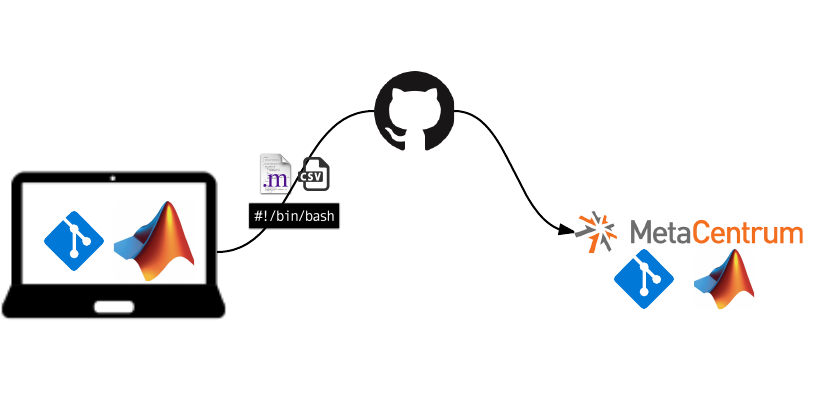
\includegraphics[scale=0.9]{up.png}
\caption{Zadávání úloh do MetaCentra.}
\label{fig:up}
\end{center}
\end{figure}


\begin{figure}[htbp]
\begin{center}
	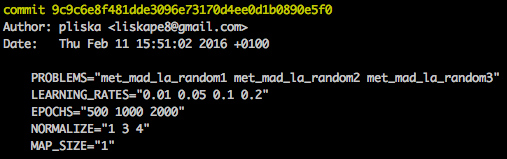
\includegraphics[scale=0.7]{semantic_commit}
\caption{Příklad strojově generovaného komentáře.}
\label{fig:semantic_commit}
\end{center}
\end{figure}



\subsubsection*{Vyzvedávání výsledků}
Kromě logů jsou do souborového systému v MetaCentru ukládany také další soubory. Po dokončení učení je celý \textit{workspace}\footnote{Workspace je množina proměnných v paměti.} serializován a uložen na disk. Stejně tak je uložena vizualizace výsledků. Protože jsou tyto výsledky uloženy na disku, je snadné je prostřednictvím Gitu přenést zpět na lokální stroj (\ref{fig:down}). Zpravidla jsou nejdříve přenášeny výsledky v obrázkových podobách -- slouží jako rychlé náhledy na výsledky. Po zhodnocení výsledků je možné vybrat konkrétní uložené workspace a přenést jej na lokální stroj. Na lokálním stroji lze workspace načíst a pokračovat v práci stejně, jako kdyby byla síť učena tam.

\begin{figure}[htbp]
\begin{center}
	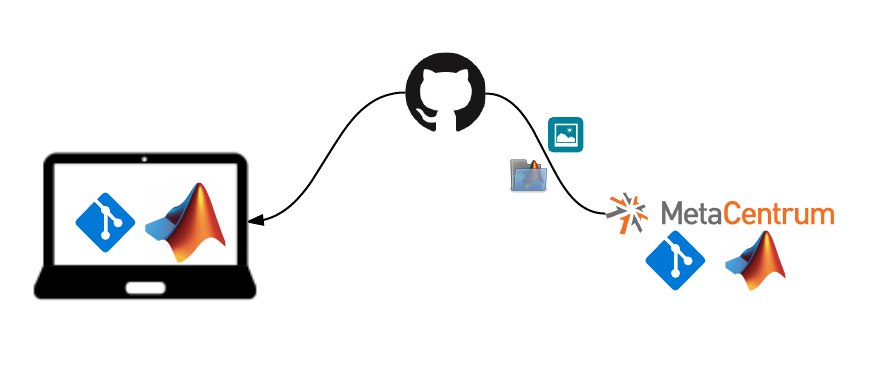
\includegraphics[scale=0.9]{down.png}
\caption{Vyzvedávání výsledků z MetaCentra.}
\label{fig:down}
\end{center}
\end{figure}


% -------------------------------------- POUŽITÁ DATA ---------------------------------------------------------------------------------------------------------------------------------------------------------------
\chapter{Použitá data a předzpracování}\label{ch:empl_prepro}
\section{Úvod do hudební problematiky}
Zvuk je mechanické vlnění v látkovém prostředí, které je schopno vyvolat sluchový vjem. Zvuky můžeme rozdělit na \textit{tóny} a \textit{hluky}. Tóny bývají označovány jako zvuky hudební, hluky jako zvuky nehudební. Tóny vznikají při pravidelném, v čase přibližně periodicky probíhajícím pohybu -- kmitání. Při jejich poslechu vzniká v uchu vjem zvuku určité výšky, proto se tónů využívá v hudbě. Tóny se dále dělí na \textit{jednoduché} -- určené jednou sinusoidou(základní) a \textit{složené} -- obsahují kromě frekvence základní navíc i tzv. vyšší harmonické. Nejdůležitějšími vlastnostmi tónu jsou: \textit{pitch(výška)}, \textit{síla(hlasitost, loudness)} a \textit{timbre(barva tónu)}.

Výška tónu je dána především frekvencí. Rozeznáváme sedm základních tónů a pět půltónů označené C, C\#, D, D\#, E, F, F\#, G, G\#, A, A\#, B, kde každý z nich představuje určitou frekvenci.

Hlasitost tónu je subjektivní veličina, která se měří v jednotce \texttt{bel[B]}.

Barva tónu je vlastnost, která umožňuje sluchem rozlišit dva složené tóny, které mohou mít stejnou absolutní výšku a které jsou vydávány dvěma různými zdroji zvuku. Je určena nejen počtem vyšších harmonických tónů obsažených ve složeném tónu, ale také jejich amplitudami. \cite{zvuk-ency}
 


% https://www.youtube.com/watch?v=mE1ZwLTZ1Bw
%http://www.wikiskripta.eu/index.php/V%C3%BD%C5%A1ka_t%C3%B3nu

\section{MillionSongDataset a The Echo Nest}
MillionSongDataset je volně dostupná kolekce hudebních atributů a metadat pro více než milion skladeb populární hudby. Tento dataset je vytvořený za účelem podpory výzkumu v oblastech algoritmů pro hudební data, MIR\footnote{Music information retrieval} a další. MillionSongDataset byl vytvořen společností The Echo Nest, která se zabývá hudební analýzou, porozuměním hudebního obsahu a vztahem hudby a posluchači. MillionSongDataset slouží jako zkratka k hudebním datům, které jinak The Echo Nest poskytuje prostřednictvím svého webového API.

	Při náročnosti metod používaných v této práci, je zřejmé, že není možné použít celý tento dataset, který má přibližně 280 GB. Manipulace s takto velkým objemem dat je velmi komplikovaná a tak zmenšování původního datasetu není vhodné řešení. Nejen z těchto důvodů byl využit konkrétní zdroj dat a to již zmíněné API. Tímto přístupem je možné jednoduše vytvářet datasety pro předem zvolené sémantiky. Takové sémantiky mohou být například žánr hudby, období vzniku, oblíbenost, autor a další. Další výhodu, kterou přinesl tento přístup, je vyšší aktuálnost metadat, zejména těch, které jsou odvozeny na základě aktuálních trendů a sociálního vnímání jako je například oblíbenost konkrétní skladby nebo míra známosti hudebního autora.
	
\section{Dostupné atributy}
\subsection{Nástroj Analyze}

Analyze je nástroj pro analýzu hudebních dat, který používá společnost The Echo Nest. 
Tento nástroj je volně dostupný prostřednictvím webového API. Vstupem programu je digitální audio soubor (např.:  mp3, m4a, wav, mpeg, flv), který je programem analyzován. Výstupní informace programu jsou poskytuty JSON souborem (\ref{json-example}), který popisuje strukturu nahrávky a hudební obsah včetně rytmu, výšek a tónů. Program využívá techniniky pro simulování fyzického a kognitivního vnímání hudby člověkem. Konkrétní fungování programu je ale proprietární. 

 Pro účely této práce je nejdůležitější analýza s názvem "segments”. Jeden segment představuje množinu zvukových entit, které jsou relativně neměnné v hudebních atributech. Segmenty jsou charakterizovány začátkem a trváním v sekundách, hlasitostí a popisem výšek a tónů:



\begin{listing}
\begin{minted}[frame=single,
               framesep=3mm,
               linenos=true,
               xleftmargin=21pt,
               tabsize=4]{js}


{  
   "meta":{  
      "analyzer_version":"3.08b", "detailed_status":"OK",
      "artist":"Michael Jackson", "album":"Thriller",
      "title":"Billie Jean", "genre":"Rock",
      "bitrate":192, "sample_rate":44100,
      "seconds":294, "status_code":0,
      "timestamp":1279120425, "analysis_time":3.83081,
      ...
   },
   "track":{  
      "duration":294.15293, "loudness":-7.078,
      "tempo":117.152, "tempo_confidence":0.848,
      "time_signature":4,
      "time_signature_confidence":0.42, "key":6,
      "key_confidence":0.019, "mode":1,
      "mode_confidence":0.416,
      ...
   },
   "bars": [...],
   "beats": [...],
   "tatums": [...],
   "sections": [...],
   "segments":
     [{ 
        "start":0.00000, "duration":0.31887,
        "confidence":1.000, "loudness_start":-60.000,
        "loudness_max_time":0.10242,
        "loudness_max":-16.511,"pitches":[0.370,
        0.067, 0.055, 0.073, 0.108, 0.082, 0.123,
        0.180, 0.327, 1.000, 0.178, 0.234],
        "timbre":[24.736, 110.034, 57.822, -171.580,
        92.572, 230.158, 48.856, 10.804,
        1.371, 41.446, -66.896, 11.207]
      },
      ... ]
}


\end{minted}
\caption{Výstup nástroje Analyze pro skladbu Billie Jean.} 
\label{json-example}
\end{listing}

\begin{description}
\item[loudness]

je reprezentována celkem třemi údaji: \textit{loudness\_start}, \textit{loudness\_max} a \textit{loudness\_max\_time}, které popořadě reprezentují: relativní hlasitost na začátku segmentu, maximální relativní hlasitost v segmentu a čas, který specifikuje nejhlasitější místo v segmentu,
 
\item[pitches] je 12-dimenzionální vektor, kde každá dimenze představuje dominanci hudebního tónu v segmentu. Hudební tóny jsou popořadě: C, C\#, D, D\#, E, F, F\#, G, G\#, A, A\#, B,

\item[timbre] je 12-dimezionální vektor reprezentující jeden segment z hlediska barev tónů. Pro účely této práce je důležité, že takové vektory jsou vhodné na porovnávání mezi sebou. Toto tvrzení a další informace o způsobu získávání vektorů, které je mimo rámec této práce, jsou k naleznutí v oficiální dokumentaci nástroje \cite{analyze},

\item[confidence] je číslo mezi 0 a 1, které symbolizuje jistotu analyzátoru pro konkrétní segment. Z důvodu zjednodušení nebude v této práci vůbec uvažován.
\end{description}

\subsection{Další atributy}
Mimo akustické atributy, které je možné získat z nástroje Analyze, The Echo Nest poskytuje velké množství dalších prostřednictví svého webového API.

Poskytované atributy je možné rozdělit do tří kategorií. První kategorie jsou metadata. Do této kategorie patří například název skladby, jméno autora nebo rok vzniku. Další kategorií jsou atributy tzv.: socilání. Do sociálních atributů jsou zařazeny míry oblíbenosti, známosti apod. Poslední kategorií jsou algoritmicky získané atributy, které popisují sladbu jako celek. Příkladem takových atributů jsou danceability (míra vhodnosti skladby pro tancování) a valence (míra pozitivní energie, kterou skladba vyzařuje).\footnote{Vyčerpávající popis dostupných atributů je k nalezení na adrese: http://developer.echonest.com/docs/v4/song.html}

\section{Výběr dat a předzpracování}
Jak ilustrují předchozí sekce, možnosti výběru dat a způsobů předzpracování jsou rozsáhlé. Nicméně z důvodu jednoduchosti byly zvoleny pouze timbre vektory, které mají ambice reprezentovat hudení znaky skladby. Při zvolení čistě akustického atributu se také předejde vytváření něchtěných závislostí mezi daty a zvolenou sémantikou. Každá skladba je reprezentována rozdílným počtem segmentů a tím pádém také rozdílným počtem timbre vektorů. Pro získání konečných atributů byla použita kovarianční matice a průměrný vektor, stejně tak jako \textit{YearPredictionMSD datasetu}\footnote{Dostupný na https://archive.ics.uci.edu/ml/datasets/YearPredictionMSD.}. Tímto přístupem je možné pro každou skladbu získat $90$ desetinných čísel, které představují reprezentaci původního objektu. 




% -------------------------------------- Experimenty ---------------------------------------------------------------------------------------------------------------------------------------------------------------
\chapter{Experimenty}
\section{Protokol}

V rámci této práce se konkrétní protokoly experimentů mohou lišit v rozdílných částech. V této sekci je uveden abstraktní protokol, který definuje nutné části a společná nastavení pro všechny experimenty. TODO: výčet

\subsubsection*{Cíl experimentu}


\subsubsection*{Vstupní data}
Pro experimentování jsou použita data, která jsou popsána v kapitole \ref{ch:empl_prepro}. Kromě předzpracování popsaného v kapitole je dále aplikovaná normalizace, jejíž význam je popsán hned v prvním experimentu (TODO).
Vstupním vektorům jsou dále přiřazeny třídy, které představují sémantiku. Jednotlivé sémantiky budou upřesněny u konkrétních experimentů.


\subsubsection*{Metody}
V experimentech jsou výhradně použity metody SOM a CRSOM. Teoretické základy a analytické vyjádření těchto metod jsou popsány v \ref{sec:som_teo} a \ref{sec:crsom_teo}. Použitá implementace je pak rozebrána v \ref{sec:som_impl} a \ref{sec:som_impl}. 



\subsubsection*{Nastavení metod}

TODO: velikost mřížek

Jak bylo popsáno v implementační části práce, pro metodu SOM byla použita samoorganizující síť dodaná v rámci neural network toolboxu. S tímto rozhodnutím bylo převzato velké množství nastavení, které je možné dohledat v dokumentaci\footnote{Dokumentace dostupná na: http://www.mathworks.com/help/nnet/ref/selforgmap.html}. Pro učení sítě SOM bylo vždy použito $200$ epoch. Mřížka neuronů v těchto sítích byla vždy pravoúhlá (\ref{fig:grid_top}).

U sítě CRSOM je proměnlivost nastavení mnohem vetší. Všechny sítě tohoto typu mají společnou inicializaci: pro počáteční nastavení prototypových vektorů byla použita metoda \texttt{initsompc}, zatímco všechny váhy v kontextové síti byly nastaveny na $0$. Další parametry jako learning rate a počet epoch byly proměnlivé a budou dospecifikovány u konkrétních experimentů.




\subsubsection*{Výsledky}

    \begin{itemize}
        \item MSE při učení CRSOM
        \item SOM mapa
        \item CRSOM mapa před učením
        \item CRSOM mapa
        \item SRI CRSOM mapy
        \item Další v závislosti na cíli experimentu
    \end{itemize}

\subsubsection*{Závěr}
Interpretace


\subsection{Semantic relevance index}
Semantic relevance index (SRI) je míra, která kvantifikuje schopnost výsledných map zachovávat sémantický význam dat v nízce dimenzionální mapě \cite{hartono14}. SRI je poměr mezi $I_{class}$ a $O_{class}$. $O_{class}$ je míra, která určuje jak moc jsou data s rozdílným významem (třídou) na mapě rozdělena (\ref{eq:oclass}). Oproti tomu $I_{class}$ udává, jak moc jsou data se stejným významem mapována k sobě (\ref{eq:iclass}).



\vspace{\baselineskip}
\noindent
\begin{minipage}[c]{\textwidth }

\begin{equation} \label{eq:sri}
    SRI=\frac{I_{class}}{O_{class}}
\end{equation}

\begin{equation} \label{eq:oclass}
	I_{class}  = \frac{1}{N}\sum_{i=1}^{N}  \| H(X_i) - H(max_{in}(X_i, j)) \|
\end{equation}


\begin{equation} \label{eq:iclass}
	O_{class}= \frac{1}{N(M-1)}\sum_{i=1}^{N}\sum_{k \neq C(X_i)} \| H(X_i) - H(min_{out}(X_i, j)) \|
\end{equation}



Kde:\\
\hspace*{3em}
\begin{tabular}{rl}
    $H(X_i)$:&  souřadnice $BMU$ na mapě pro vstupní vektor $X_i$  \\
    $min_{out}(X_i, j)$: & nejbližší vstupní vektor k $X_i$ s třídou $j$  \\
     $C(X_i)$:& třída vektoru  $X_i$\\
     $N$, $M$:& počet vstupních vektorů, počet tříd\\
     $max_{in}(X_i)$:& vektor s třídou $C(X_i)$ a nejvyšší vzdáleností od $X_i$ \\
\end{tabular}
\end{minipage} 
\vspace{\baselineskip}
\noindent


  
\section{Učení CRSOM}
V této sekci jsou rozebrány některé aspekty učení CRSOM. Jako první téma je vliv normalizace vstupních dat na učení sítě. Dále je studován průběh učení CRSOM z pohledu chyby na výstupu sítě a nakonec formování mapy a význam kontextové sítě.



\subsection{Normalizace dat a učení CRSOM}

Skutečnost, že učení CRSOM je citlivé na nastavení učících parametrů (např.: learning rate), je experimentálně ukázáno v \cite{hartono14}. Při implementaci CRSOM byla zjištěna další citlivost a to na způsobu normalizace dat.
Cílem experimentu je ukázat závislost způsobu normalizace dat a průběhu učení a tyto závislosti interpretovat. 
Pro účel tohoto experimentu byl zvolen KatyRamDataset (\ref{app:KatyRamDataset}). Všechny sítě v této sekci byly učeny s $LR=0.1$ po $500$ epoch.


\begin{figure}
\centering
\begin{subfigure}{.5\textwidth}
  \centering
  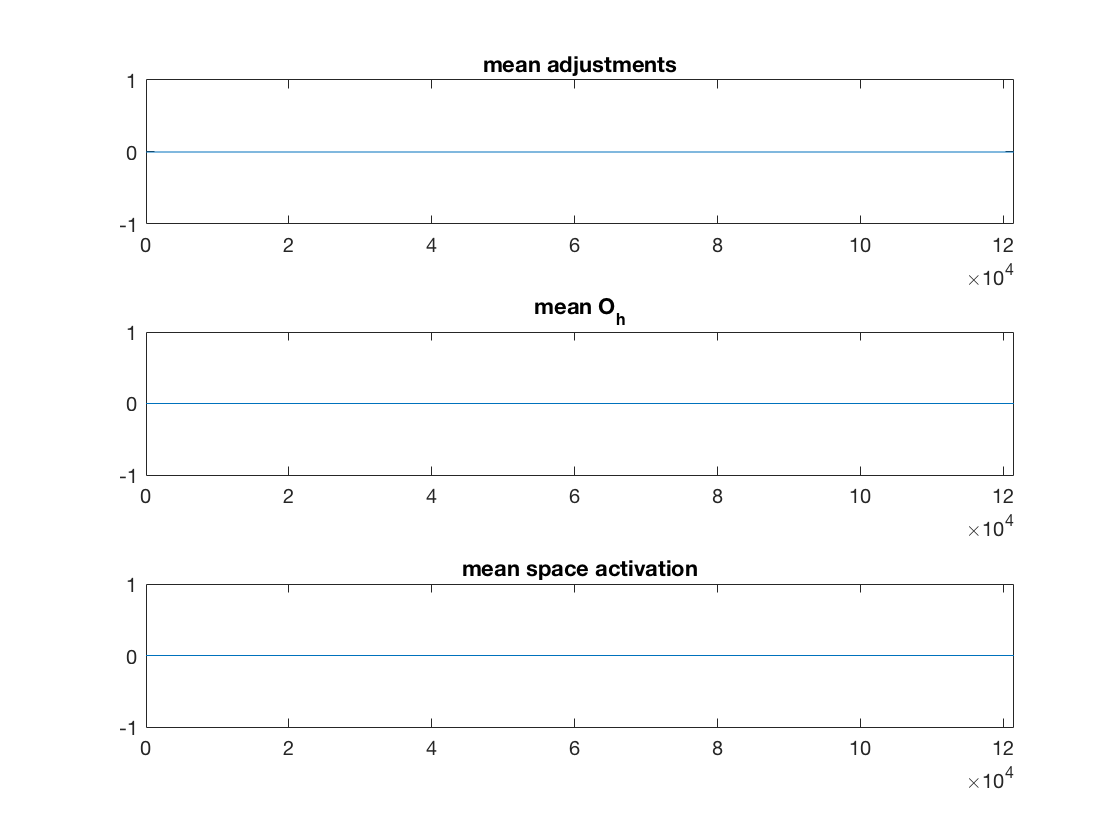
\includegraphics[width=.99\linewidth]{norm-learnattrs0.png}
  \caption{Veličiny učení}
  \label{fig:learnattrs0}
\end{subfigure}%
\begin{subfigure}{.5\textwidth}
  \centering
  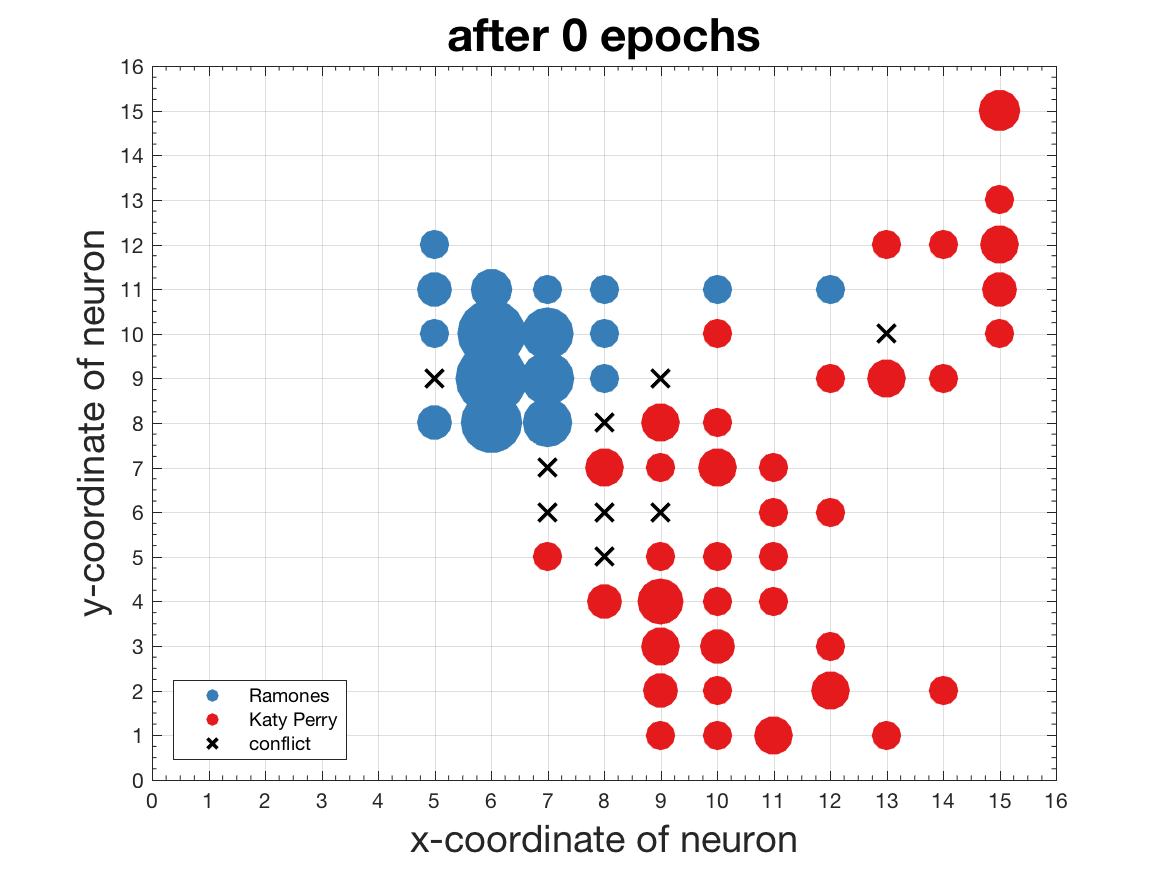
\includegraphics[width=.99\linewidth]{exp_kp_ram_norm_0.png}
  \caption{Sémantická mapa}
  \label{fig:resmap0}
\end{subfigure}
\caption{Výsledky pro učení bez normalizace}
\label{fig:nonorm}
\end{figure}


\subsubsection*{Bez normalizace dat}\label{sec:nonorm}

V této sekci je rozebráno chování sítě CRSOM bez použití jakékoliv normalizace. Stejně tak jako pro všechny ostatní přístupy jsou zobrazeny obrázky (\ref{fig:nonorm}) definující učení a výslednou mapu. Obrázek vlevo (\ref{fig:learnattrs0}) se skládá ze tří podobrázků. Na každém je vykreslena jedna veličina učení. Na horním podobrázku je vykresleno průměná úprava prototypových vah. Na prostředním podobrázku je vykreslena průměrná hodnota výstupu skryté vrtsvy $O_h$. Na dolním podobrázku je pak vykreslena průměrná prostorová aktivace $e^{-\mathcal{I}_i^h(t)}$. Obrázek vpravo (\ref{fig:resmap0}) pak zobrazuje výslednou sémantickou mapu.



Vysoce dimenzionální prostor zapříčinil obrovské absolutní vzdálenosti mezi vstupními vektory a nainicializovanými prototypovými vektory. Tím pádem je velikost $e^{-\mathcal{I}_i^h(t)}$ vždy zanedbatelně málá, v reprezentaci matlabovských čísel je rovna $0$. To implikuje nulový výstup ze skryté vrstvy respektive nulové úpravy prototypových vektorů. Sémantická mapa (\ref{fig:resmap0}) tak pouze zobrazuje počáteční stav prototypových vektorů. Hlavním cílem normalizace dat bude zredukovat absolutní velikosti vektorů.




\subsubsection*{Normalizace pomocí \texttt{mapminmax}}
\texttt{mapminmax}\footnote{Dokumentace na: http://www.mathworks.com/help/nnet/ref/mapminmax.html} je funkce dostupná v matlabu a normalizuje vektor tak, aby maximum a minimum vektoru bylo rovnu předem stanoveným konstantám.



Byly zkoumány průběhy učení a výsledky pro různé nastavení těchto konstant. Minimum bylo vždy $0$ a pro maxima byly voleny hodnoty $max\in\{0.1, 0.2, \dots, 1.6\}$. Jednotlivé atributy tak byly normalizovány do intervalu $[0; max]$.  Výsledné SRI pro naučené sítě jsou zaneseny v tabulce \ref{tab:sri}. Na obrázku \ref{fig:sriscatter} jsou vynesené dvojice hodnot: $max$ a příslušné výsledné SRI odpovídající sémantické mapě naučené CRSOM sítě. Horizontální přímka v hodnotě $0.3749$ představuje hodnotu SRI pro nenatrénovanou (pouze inicializovanou) mapu. 

\vspace{\baselineskip}
\noindent
\begin{minipage}{\textwidth}
  \begin{minipage}[b]{0.19\textwidth}
  \centering
        \begin{tabular}{|l|c|}
        \hline
        \multicolumn{1}{|c|}{max}                     & SRI  \\ \hline
        {\color[HTML]{000000}  1.6 } & {\color[HTML]{000000} 0.3749} \\ \hline
              1.5                        &  0.3749                      \\ \hline
          1.4                        &  0.3749                      \\ \hline
          1.3                        &  0.3749                      \\ \hline
        1.2                        &  0.3709                      \\ \hline
        1.1                        & 0.3230                      \\ \hline
        1.0                        & 0.0448                      \\ \hline
        0.9                        & 0.2288                      \\ \hline
        0.8                        & 0.2028                      \\ \hline
        0.7                        & 0.8640                      \\ \hline
        0.6                        & 0.8030                      \\ \hline
        0.5                        & 0.7341                      \\ \hline
        0.4                        & 1.2298                      \\ \hline
        0.3                        & 1.1536                      \\ \hline
        0.2                        & 0.6344                      \\ \hline
        0.1                        & 1.1069                      \\ \hline
        
        \end{tabular}
      \captionof{table}{}
      \label{tab:sri}
    \end{minipage}
  \hfill
  \begin{minipage}[b]{0.79\textwidth}
    \centering
    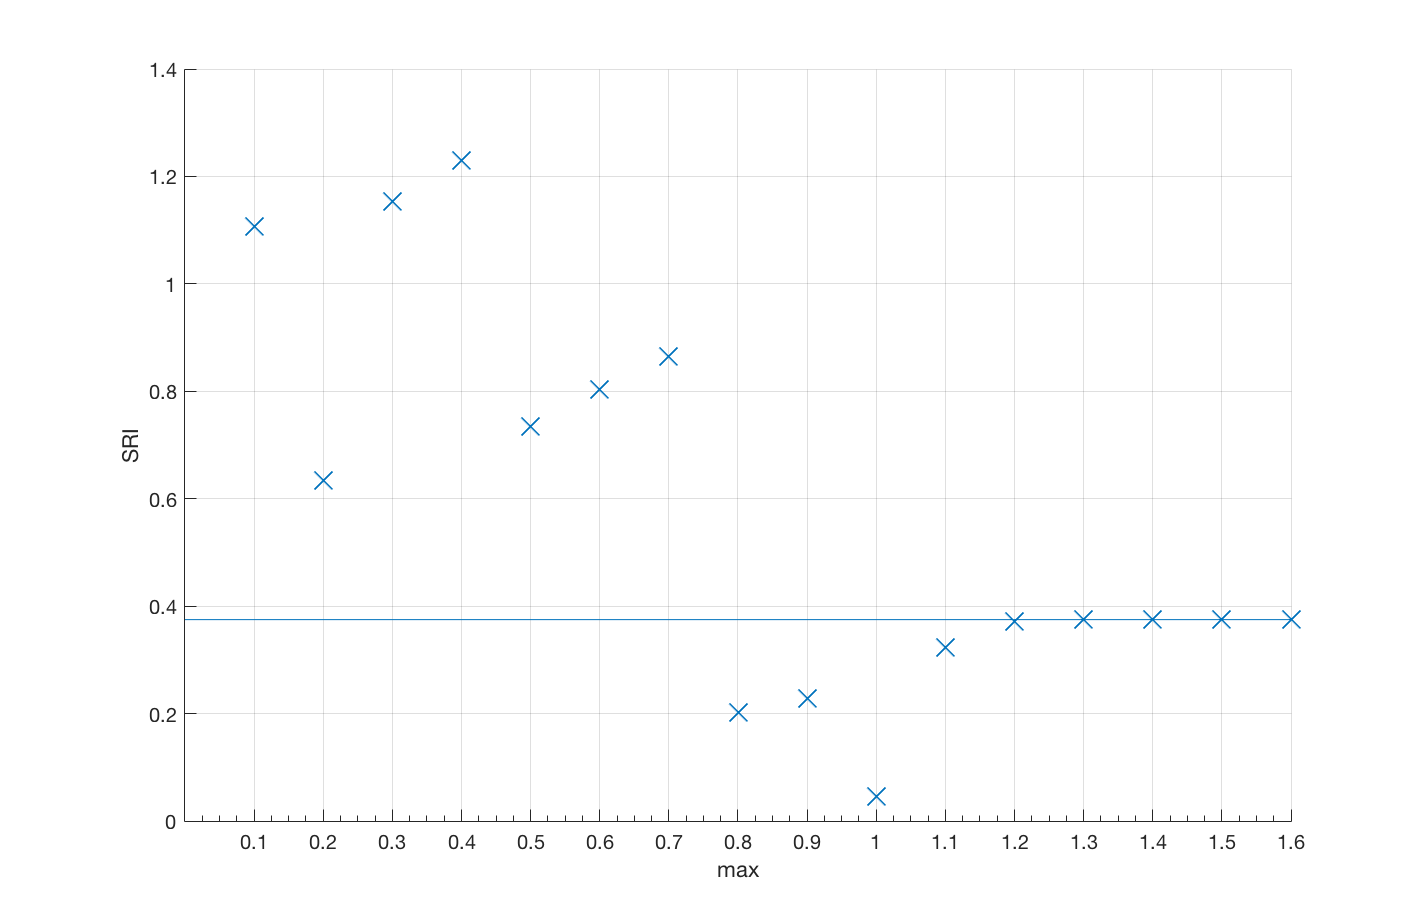
\includegraphics[scale=0.2]{sri_scatter.png}
    \captionof{figure}{}
    \label{fig:sriscatter}
  \end{minipage} 
  \end{minipage}
\vspace{\baselineskip}
\noindent


Z výsledků je možné vypozorovat skutečnost, že hodnotám $max\geq1.3$ odpovídá $SRI=0.3749$, což je shodná hodnota s nenormalizovanou mapu. Přestože jsou hodnoty prostorové aktivace nenulové (\ref{fig:attrs1300}), pohybují se v řádech $10^{-4}$, což zapříčiňuje tak malé úpravy prototypových vektorů (v řádech $10^{-11}$), že se po učení se stanoveným počtem epoch mapa vůbec nezmění (\ref{fig:map1300}).




\begin{figure}
\centering
\begin{subfigure}{.5\textwidth}
  \centering
  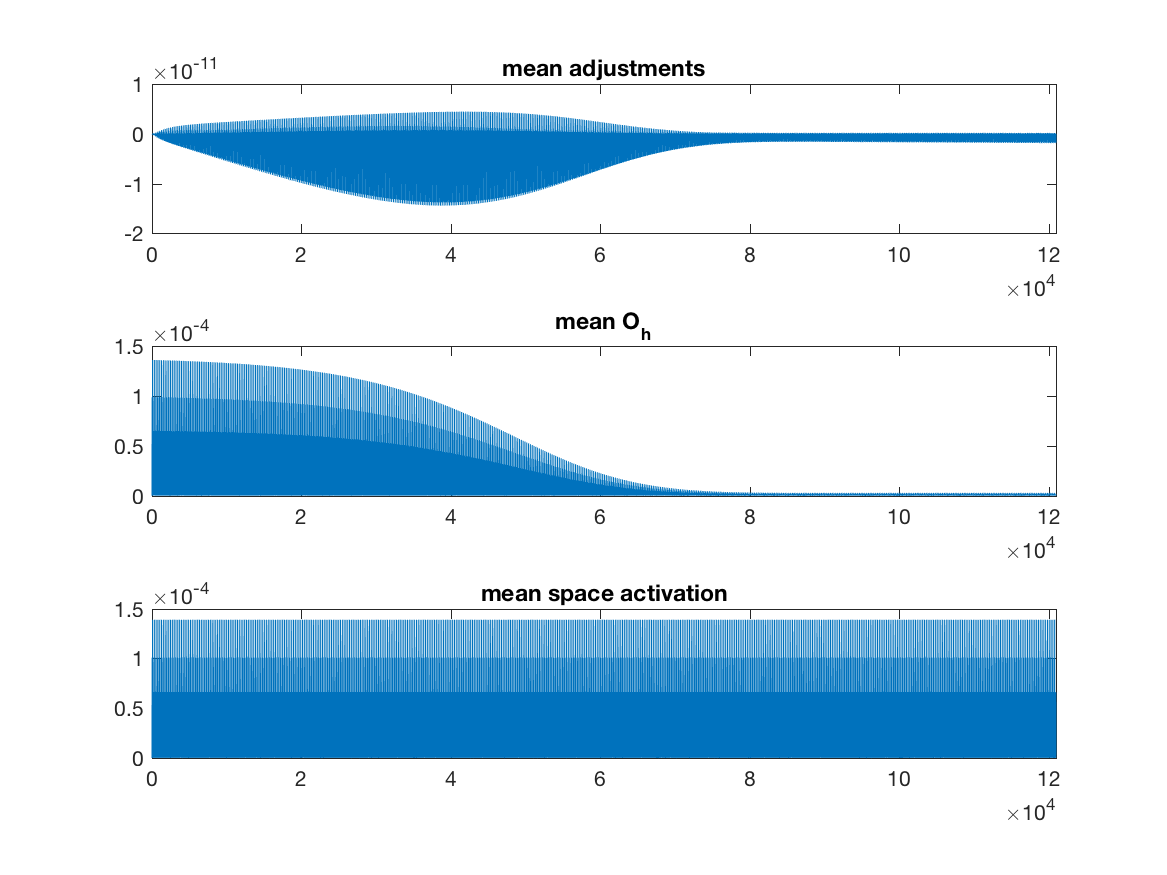
\includegraphics[width=.99\linewidth]{norm-learnattrs1300.png}
  \caption{Veličiny učení}
  \label{fig:attrs1300}
\end{subfigure}%
\begin{subfigure}{.5\textwidth}
  \centering
  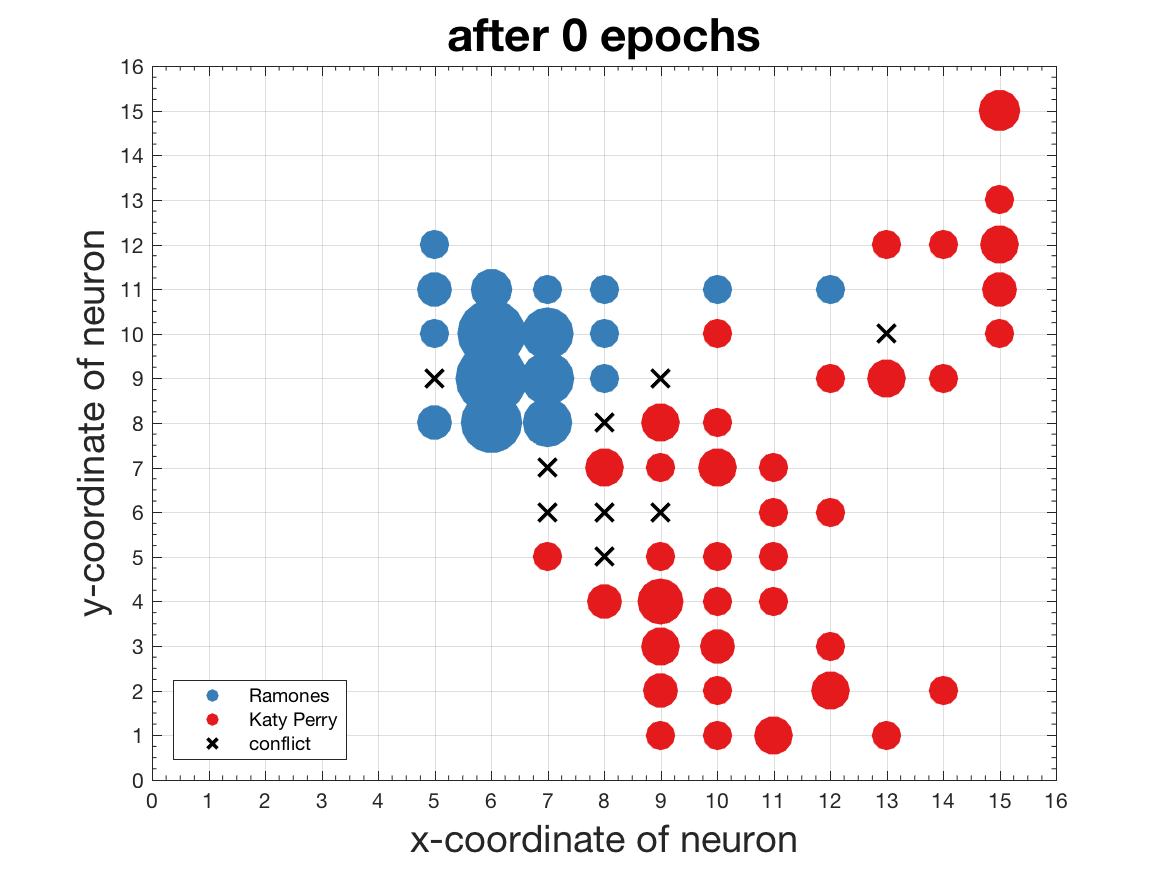
\includegraphics[width=.99\linewidth]{exp_kp_ram_norm_0.png}
  \caption{Sémantická mapa}
  \label{fig:map1300}
\end{subfigure}
\caption{Výsledky pro $max=1.3$}
\label{fig:res1300}
\end{figure}




Nejnižší hodnota SRI odpovídá $max=1.0$. Na výsledné mapě (\ref{fig:map1000}) je vidět dominantní neuron s pozicí na mřížce $[6,9]$, který se stal BMU pro většinu vstupních dat. Tuto skutečnost lze vysvětlit tak, že tento neuron byl již od počátku učení aktivován nejvíce a navíc byl v obklopení neuronů, kterým byla přiřazena stejné sémantika, tím pádem byl přibližován mnohem větší silou, než ostatní neurony. Toto tvrzení je podloženo obrázkem \ref{fig:plotsompos1000} který zobrazuje první dvě dimenze prototypových vektorů spolu se vstupními daty.

\begin{figure}
\centering
\begin{subfigure}{.5\textwidth}
  \centering
  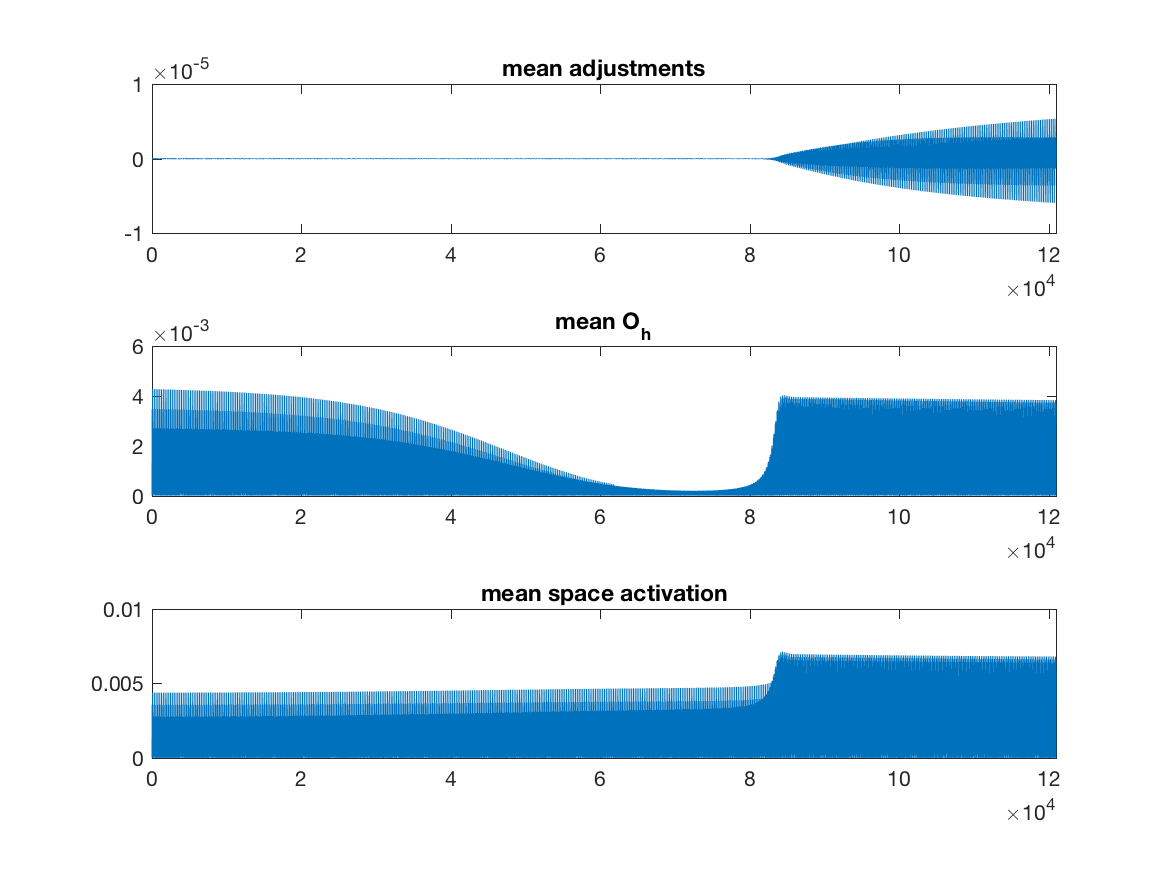
\includegraphics[width=.99\linewidth]{norm-learnattrs1000.png}
  \caption{Veličiny učení}
  \label{fig:attrs1000}
\end{subfigure}%
\begin{subfigure}{.5\textwidth}
  \centering
  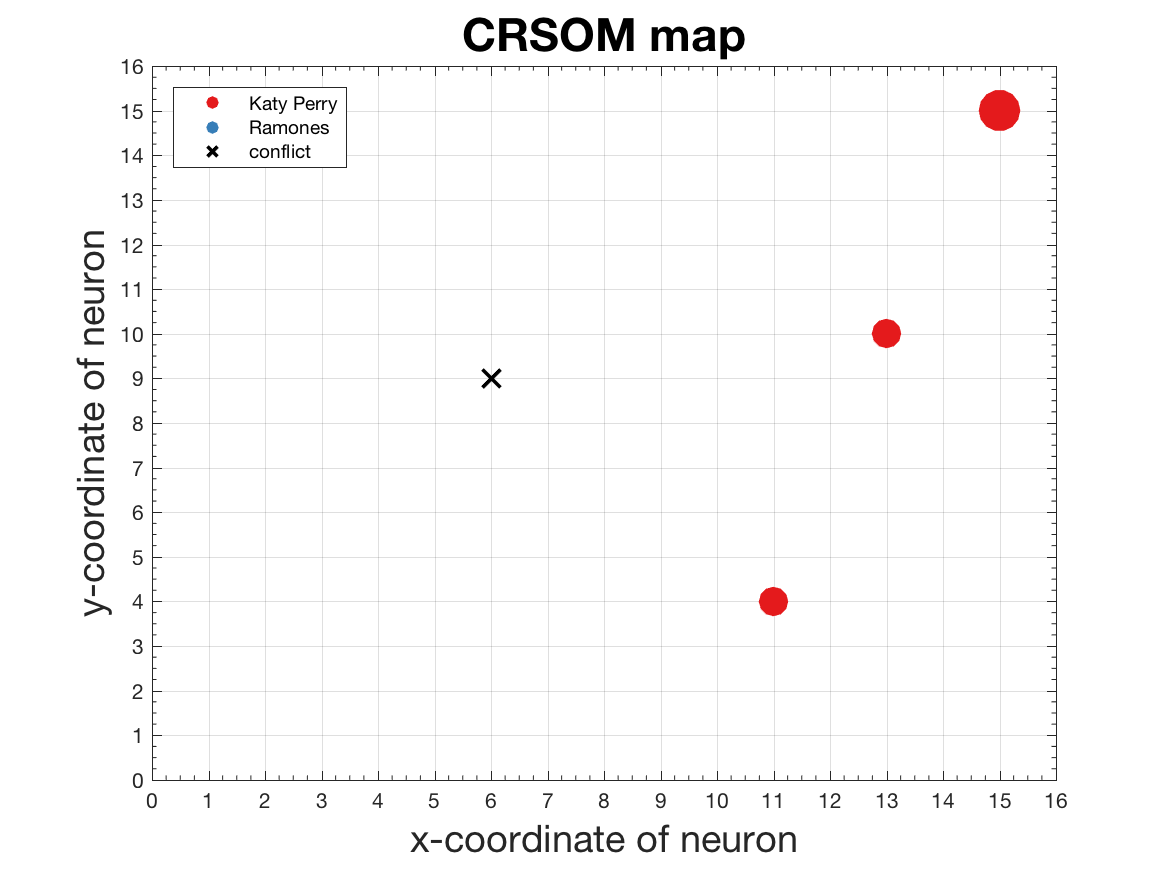
\includegraphics[width=.99\linewidth]{exp_kp_ram_1000_crsom.png}
  \caption{Sémantická mapa}
  \label{fig:map1000}
\end{subfigure}
\caption{Výsledky pro $max=1.0$}
\label{fig:res1000}
\end{figure}

\begin{figure}[htbp]
\begin{center}
	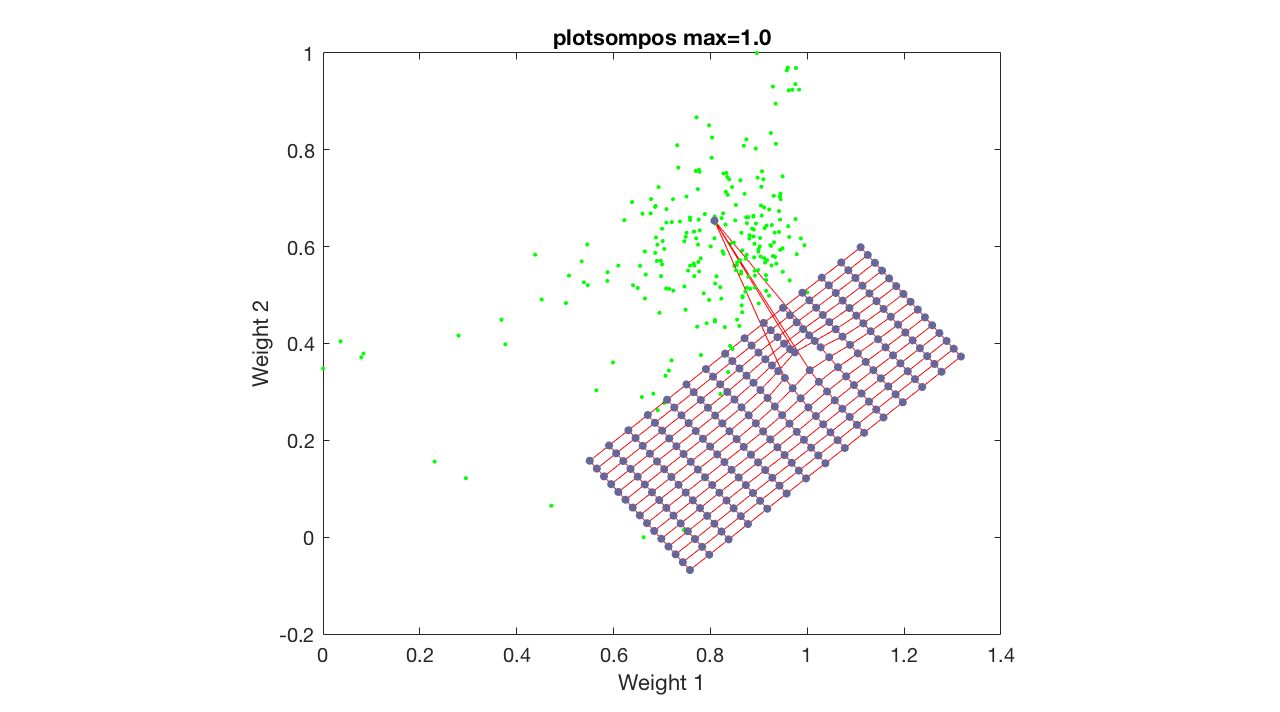
\includegraphics[scale=0.2]{plotsompos1000.png}
\caption{Dominantní neuron}
\label{fig:plotsompos1000}
\end{center}
\end{figure}


Nejvyšší hodnota SRI odpovídá $max=0.4$. Výsledná sémantická mapa (\ref{fig:resmap400}) již odpovídá očekávaní. TODO: rozebrat dále 

\begin{figure}
\centering
\begin{subfigure}{.5\textwidth}
  \centering
  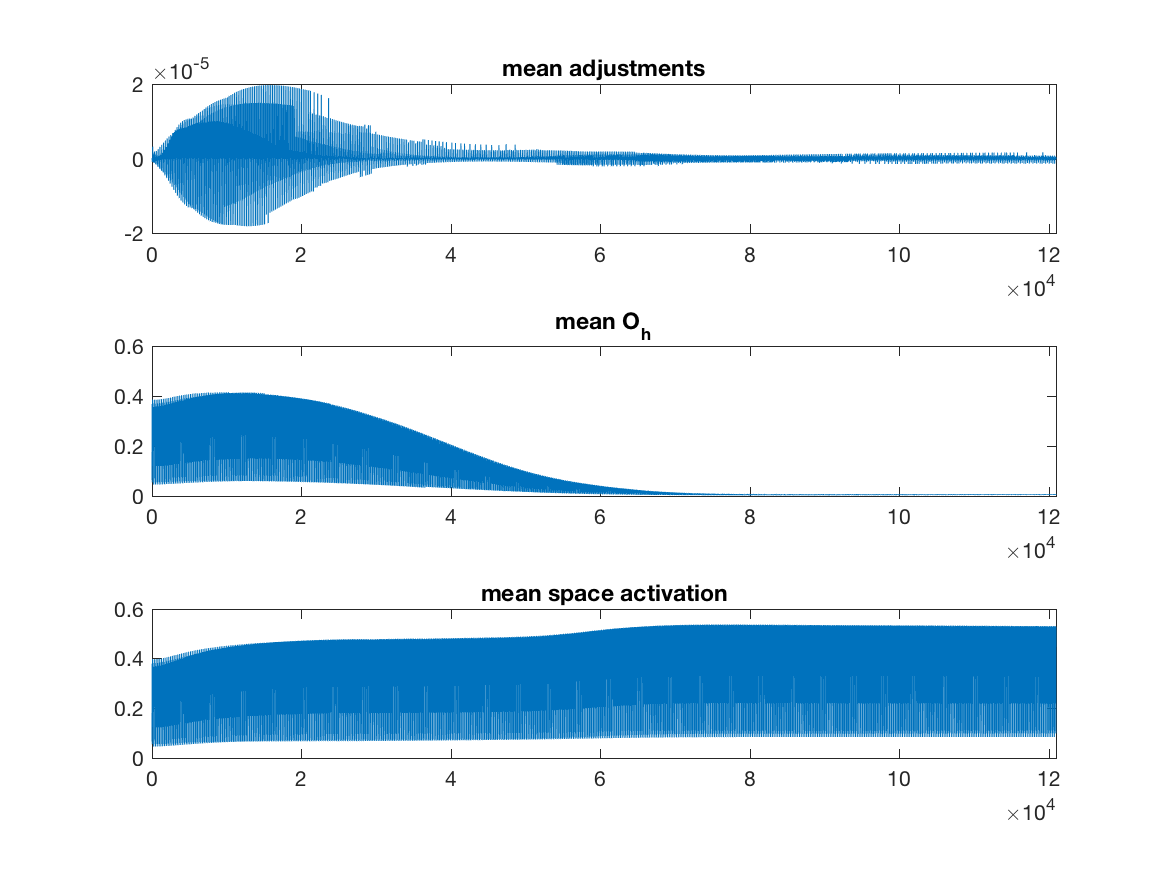
\includegraphics[width=.99\linewidth]{norm-learnattrs400.png}
  \caption{Veličiny učení}
  \label{fig:sub1}
\end{subfigure}%
\begin{subfigure}{.5\textwidth}
  \centering
  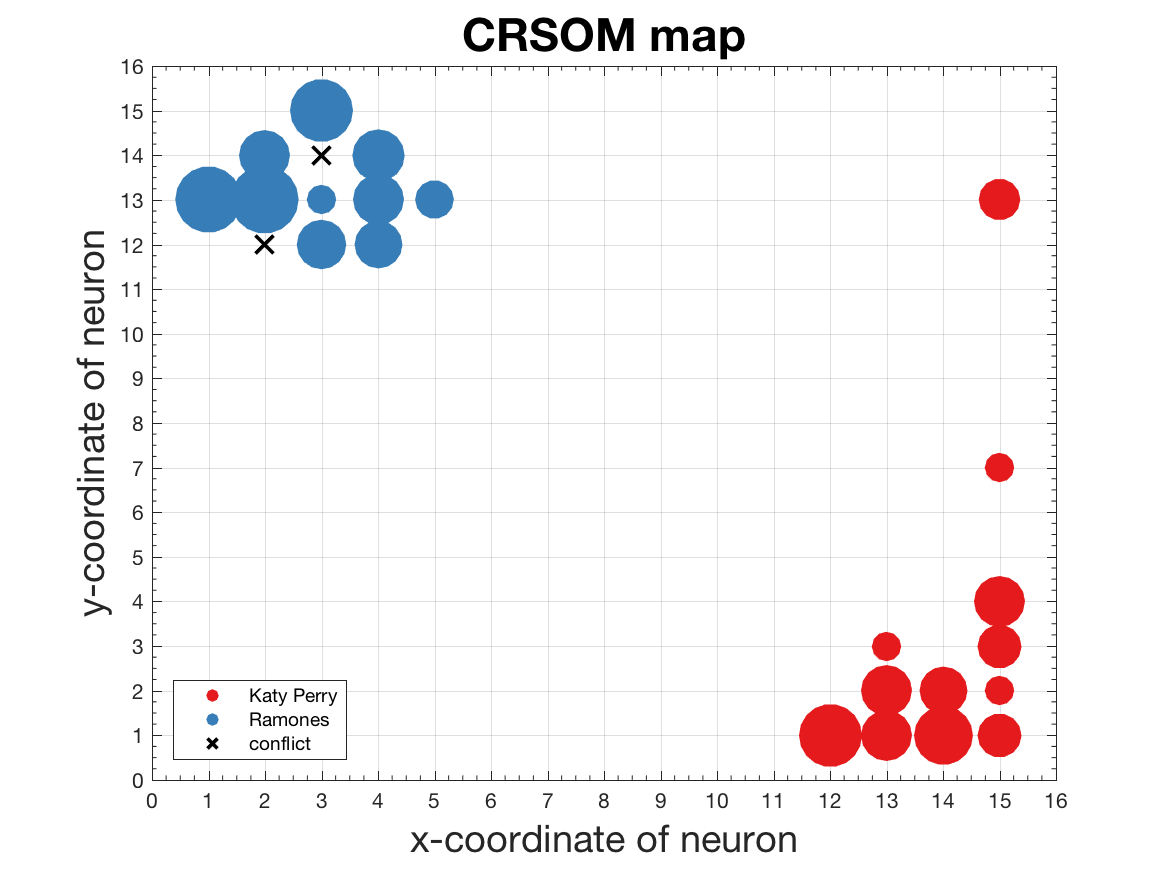
\includegraphics[width=.99\linewidth]{exp_kp_ram_crsom.png}
  \caption{Sémantická mapa}
  \label{fig:resmap400}
\end{subfigure}
\caption{Výsledky pro  $max=0.4$}
\label{fig:top}
\end{figure}


Tyto experimenty prokázaly citlivost učení CRSOM na normalizaci dat. Bez použití normalizace nedocházelo k žádným úpravám prototypových vektorů, proto se tento přístup ukázal jako nevhodný. Pro normalizaci bylo použito mapování atributů do předem zvoleného intervalu, jehož velikost byla empiricky testována. Testy ukázaly nutnost normalizace vstupních dat, nicméně není možné na jejich základě určit přesnou hodnotu $max$, která by vyhovovala obecně pro všechny problémy. Z toho důvodu se bude k hodnotě $max$ přistupovat jako k ostatním učícím parametrům a pro každý problém se bude hledat vhodná hodnota.





\subsection{Průběh učení CRSOM}
V této sekci bude studováno formování mapy pro síť CRSOM z předchozí sekce s $max=0.4$, jejíž výsledná sémantická mapa je na obr. \ref{fig:resmap400}. 

\begin{figure}[htbp]
    \begin{center}
	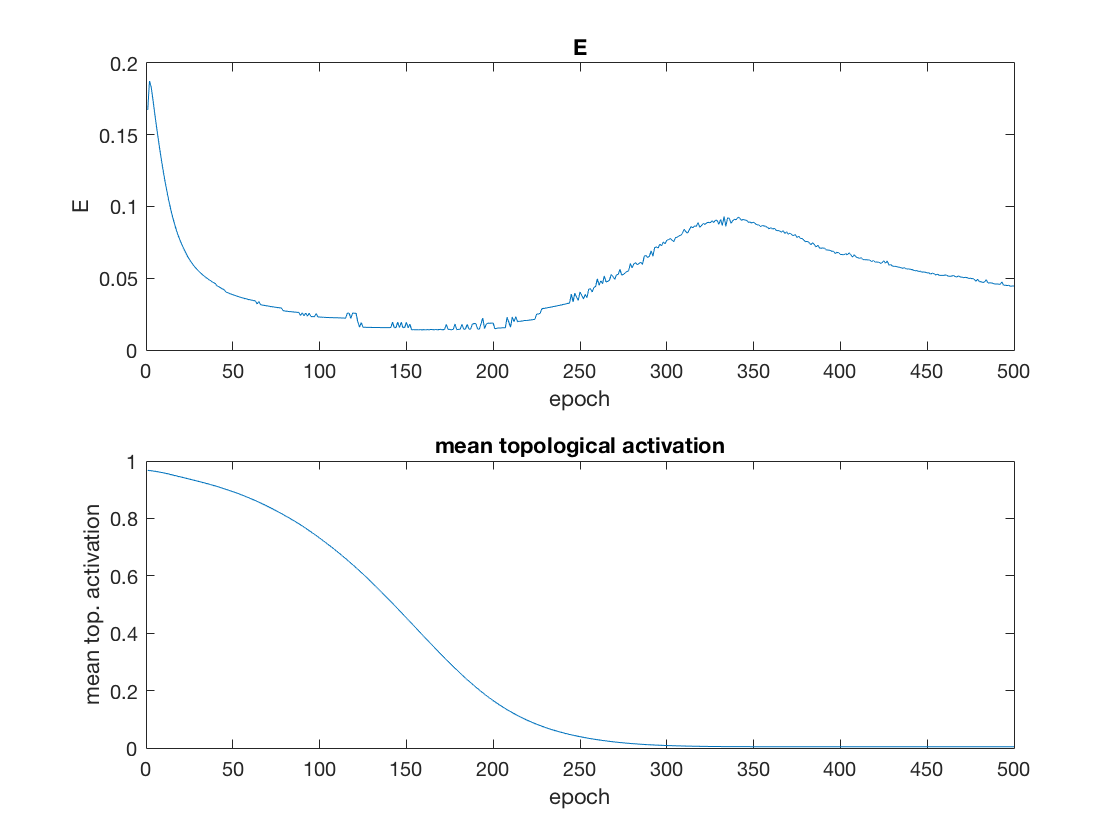
\includegraphics[scale=0.25]{mse_top.png}
	
    \caption{Průměrná chyba sítě (nahoře), pruměrná topologická aktivace (dole)} 
    \end{center}
     \label{fig:msetopp}
\end{figure}

\subsubsection*{Chyba sítě}
Chyba sítě CRSOM již byla nadefinována vztahem \ref{eq:e}. Na obrázku (\ref{fig:msetopp} nahoře) je zobrazena průměrná chyba sítě pro všechny epochy. Nemonotóní tvar této křivky je možné vysvělit následovně. Při klasické aplikaci metody nejstrmějšího sestupu se optimalizuje funkce vstupního prostoru a vah. Epochy mají navzájem stejnou množinu vstupů a úpravy vah podle gradientu nám zaručí nerostoucí průměrnou chybu.


Oproti tomu při učení sítě CRSOM do funkce $E$ vstupuje ještě další parametr -- pořadí epochy. Tím se řídí \textit{topologická aktivace} neuronů, kerá s rostoucím pořadím epochy klesá -- a to exponenciálně. Tím pádem je funkce $E$ definována pro rozdílné epochy různě a není pravda, že celková chyba sítě musí monotóně klesat.


Nárůst chyby, který je možný vidět  v rozmezí $200$-$250$ epochy, je možné vysvětlit prudkým poklesem topologické aktivace (\ref{fig:msetopp} dole). Následná opětovná konvergence $E$ k 0 je způsobená reakcí kontexové sítě na nastalou situaci a učení vah a biasu. V této fázi je již upravován pouze BMU.









\subsubsection*{Kontextová síť}
V této sekci bude studována kontextová síť. Kontextová síť se mimo jiné skládá z propojení neuronů ze skryté vrstvy a tolika výstupních složek, jako je počet tříd vstupních vektorů. Třídy, které představují sémantický kontext učení, jsou zakódovány v kódu \textit{1 z N} a proto každá výstupní složka představuje jednu třídu. Váhu  $v_{ik}$ tak lze interpretovat jako příslušnost $i$-tého neuronu k třídě $k$. 
Na obrázku \ref{fig:citizenship} jsou vizualizovány tyto příslušnosti neuronů k jednotlivým třídám. Značka na diskrétní pozici $[x;y]$ představuje jeden neuron s pozicí $[x;y]$ v mřížce. Barva značky určuje třídu příslušnosti (modrá Katy Perry, zelená Ramones) a velikost určuje míru jistoty této příslušnosti.
Na prvním obrázku jsou zobrazeny příslušnosti před učením síťe. Protože jsou váhy inicializovány na $0$, žádný neuron nepřísluší žádné třídě. S přibývajícími epochami je zřetelné rozdělování neuronů do dvou sfér vlivu, kde každá ze sfér odpovídá jedné třídě. 





\begin{figure}[htp]
    \centering
    
    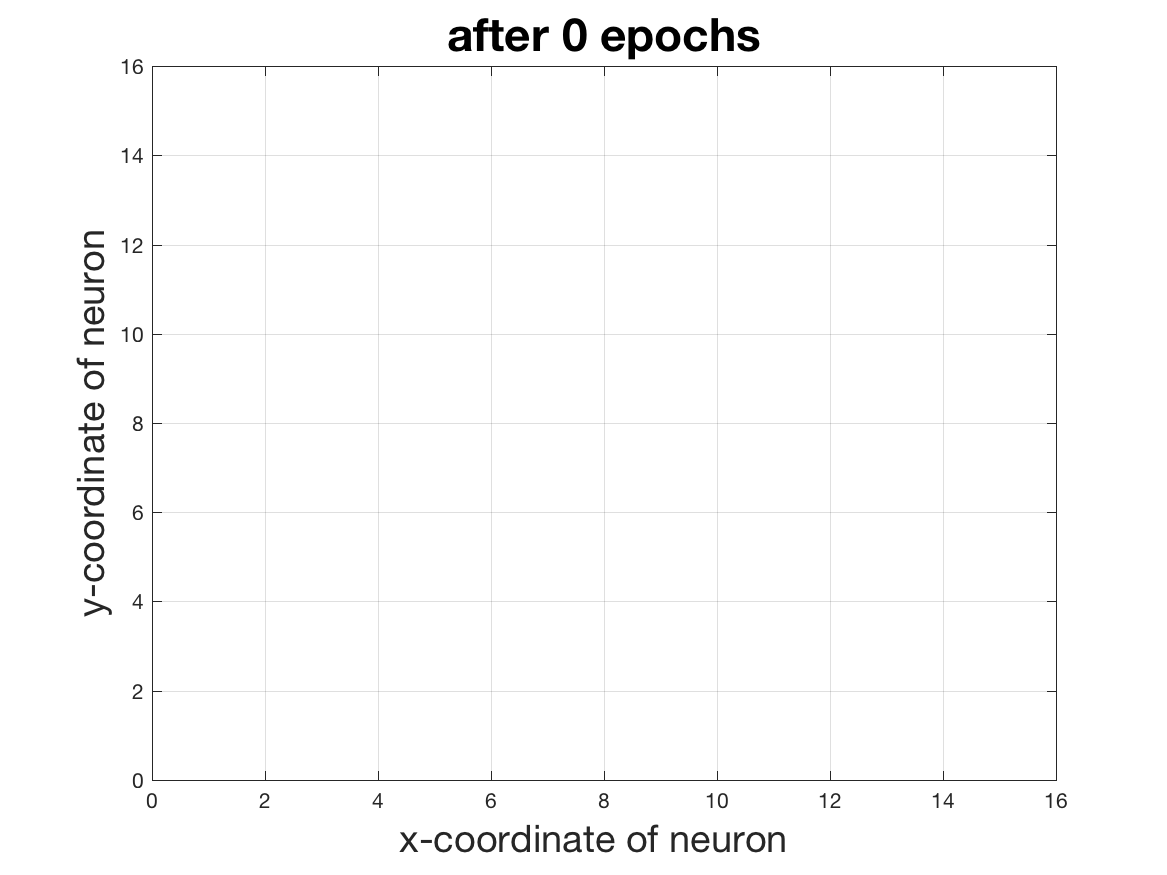
\includegraphics[width=.32\textwidth]{exp_kp_ram_citi_0.png}
    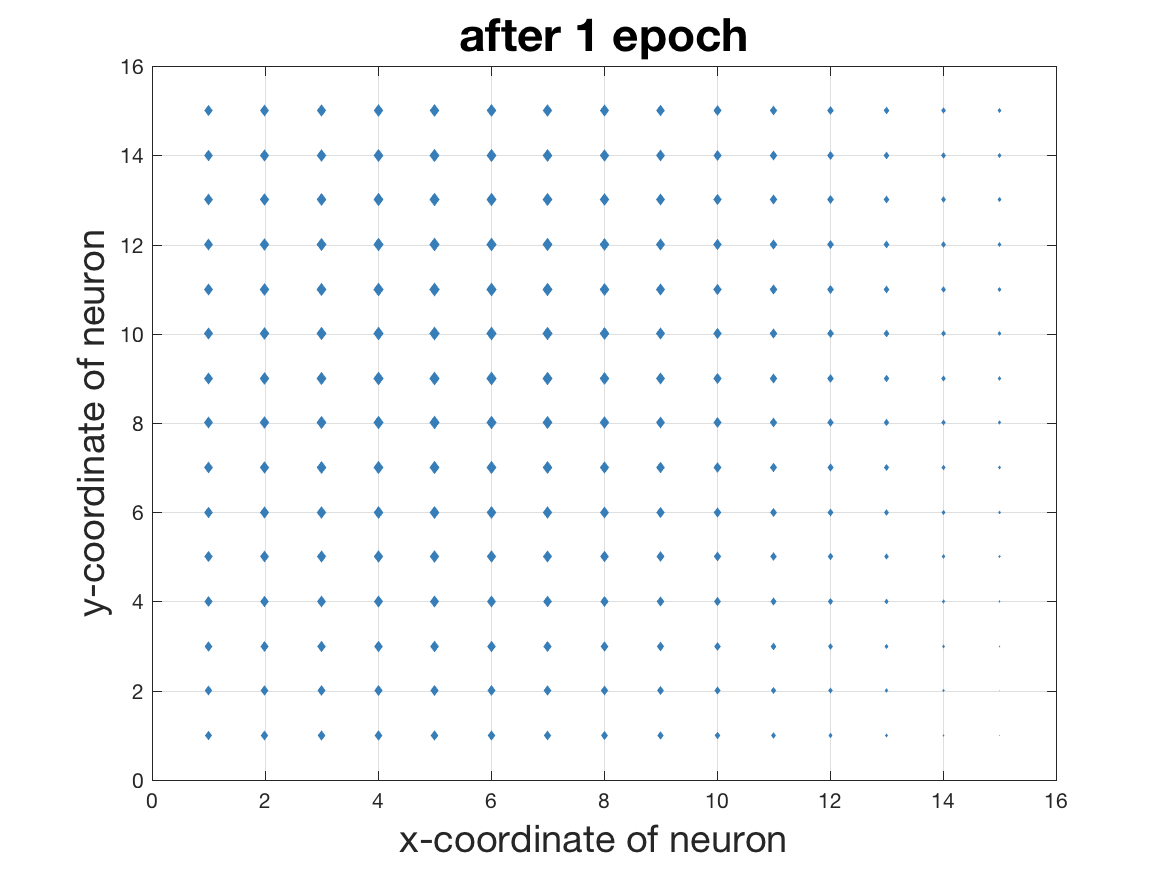
\includegraphics[width=.32\textwidth]{exp_kp_ram_citi_1.png}
    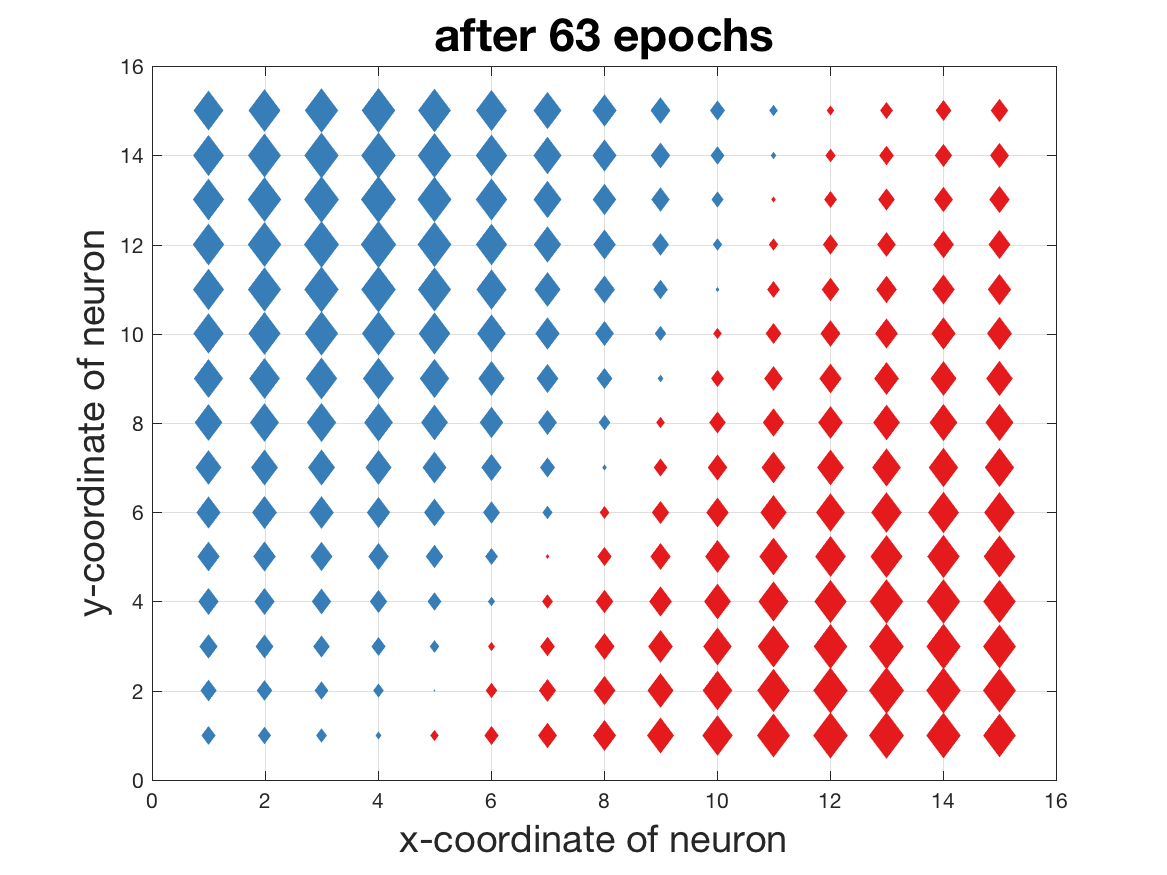
\includegraphics[width=.32\textwidth]{exp_kp_ram_citi_63.png}
        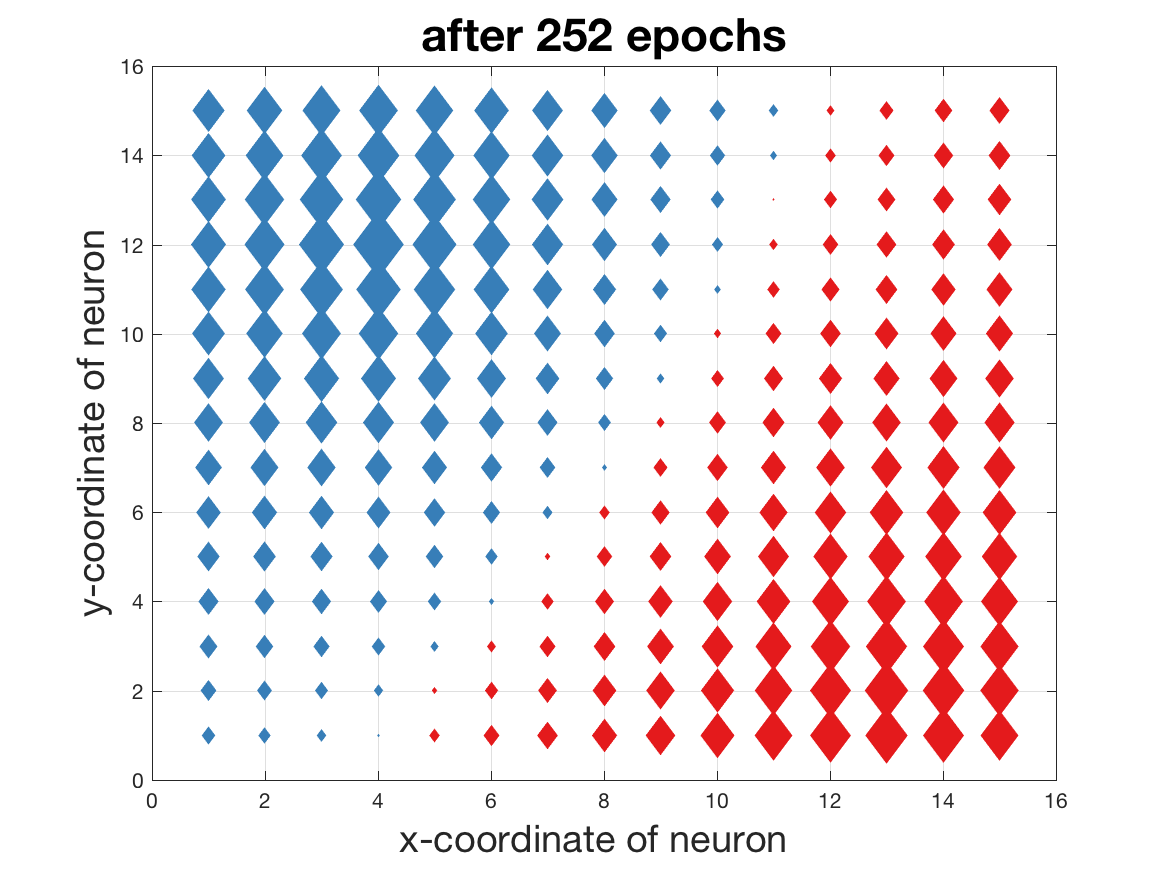
\includegraphics[width=.32\textwidth]{exp_kp_ram_citi_252.png}
    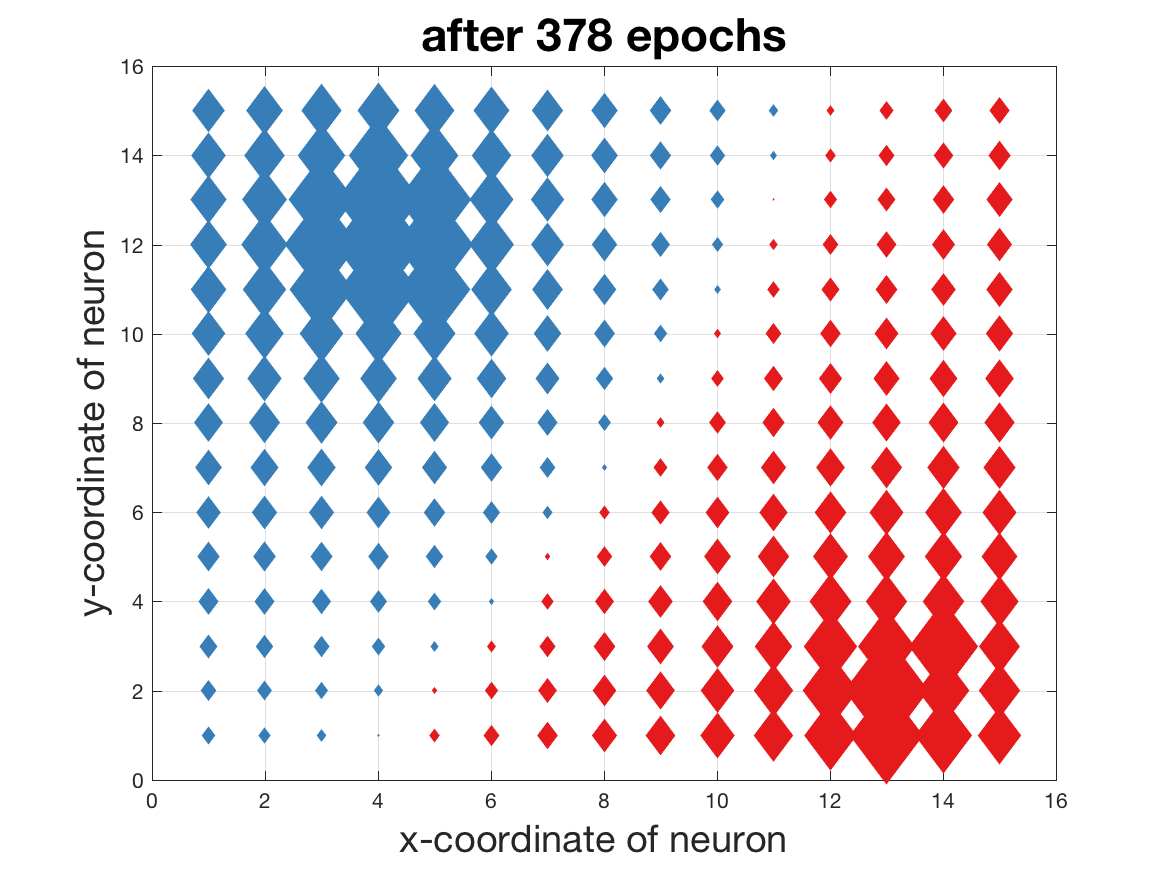
\includegraphics[width=.32\textwidth]{exp_kp_ram_citi_378.png}
    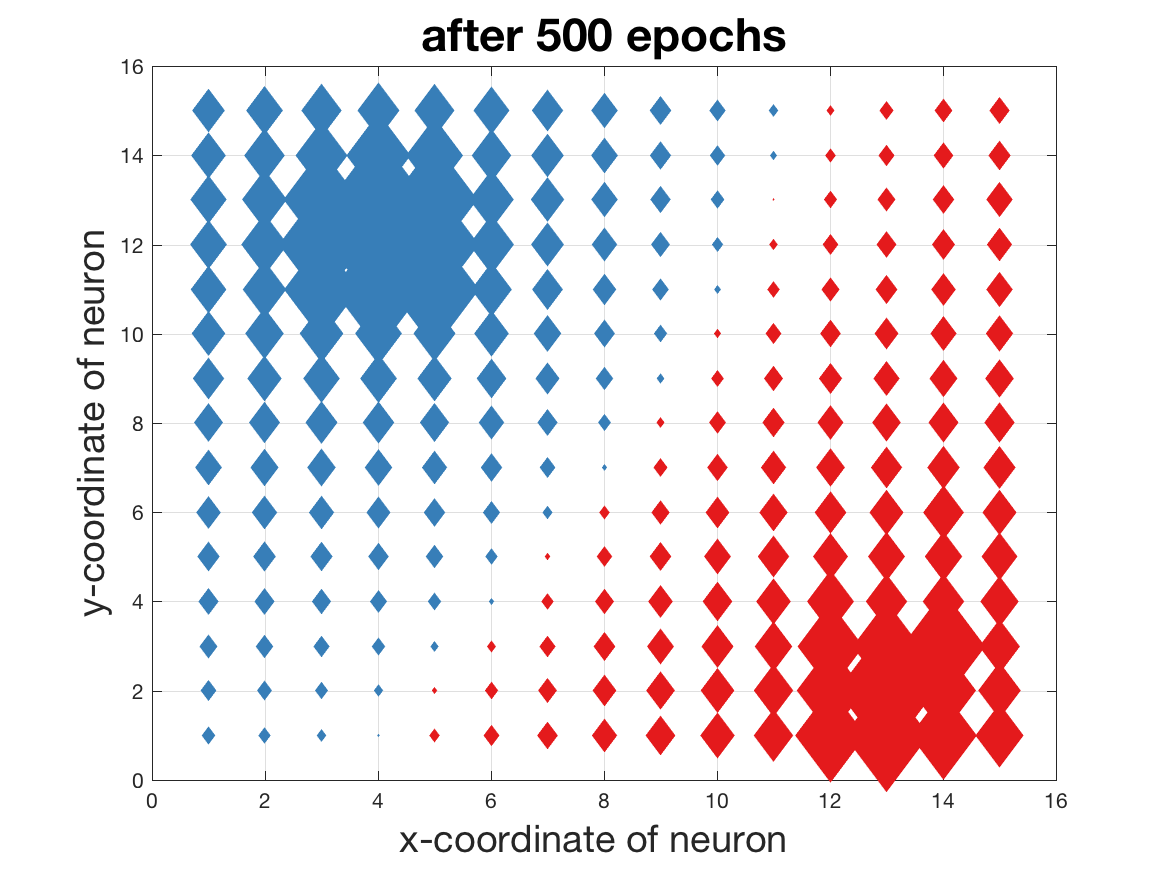
\includegraphics[width=.32\textwidth]{exp_kp_ram_citi_500.png}
    \caption{Příslušnost neuronů k třídám.}
    \label{fig:citizenship}
\end{figure}

\subsubsection*{Průběh učení}
Obrázek \ref{fig:mapform} zobrazuje formování sémantické mapy pro tytéž epochy jako na obrázku \ref{fig:citizenship}. První z obrázku odpovídá nainicalizované síti a poslední síti po uběhnutí všech $500$ epoch.
Ve stejné chvíle jsou na obrázku \ref{fig:mappos} zachyceny první dvě dimenze prototypových vektorů spolu se vstupními daty.



\begin{figure}[htp]
    \centering
    
    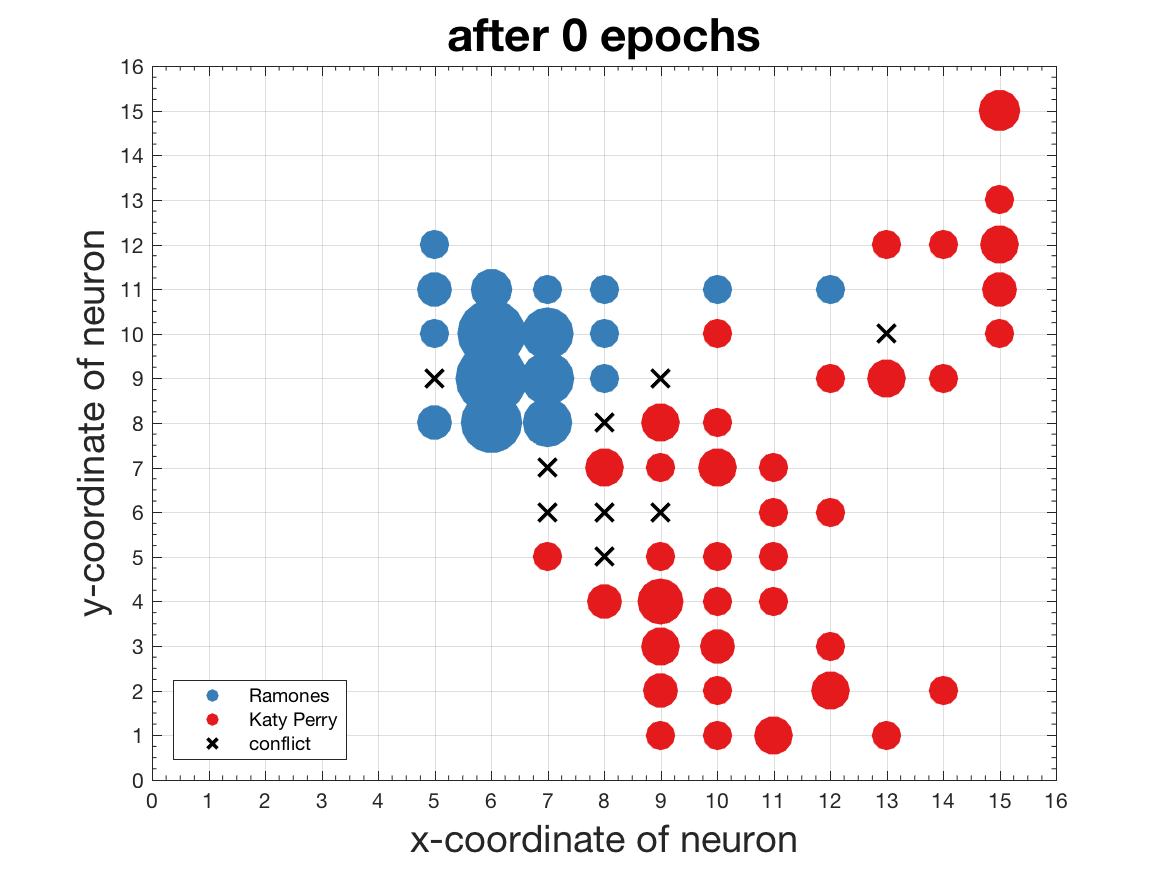
\includegraphics[width=.32\textwidth]{exp_kp_ram_norm_0.png}
        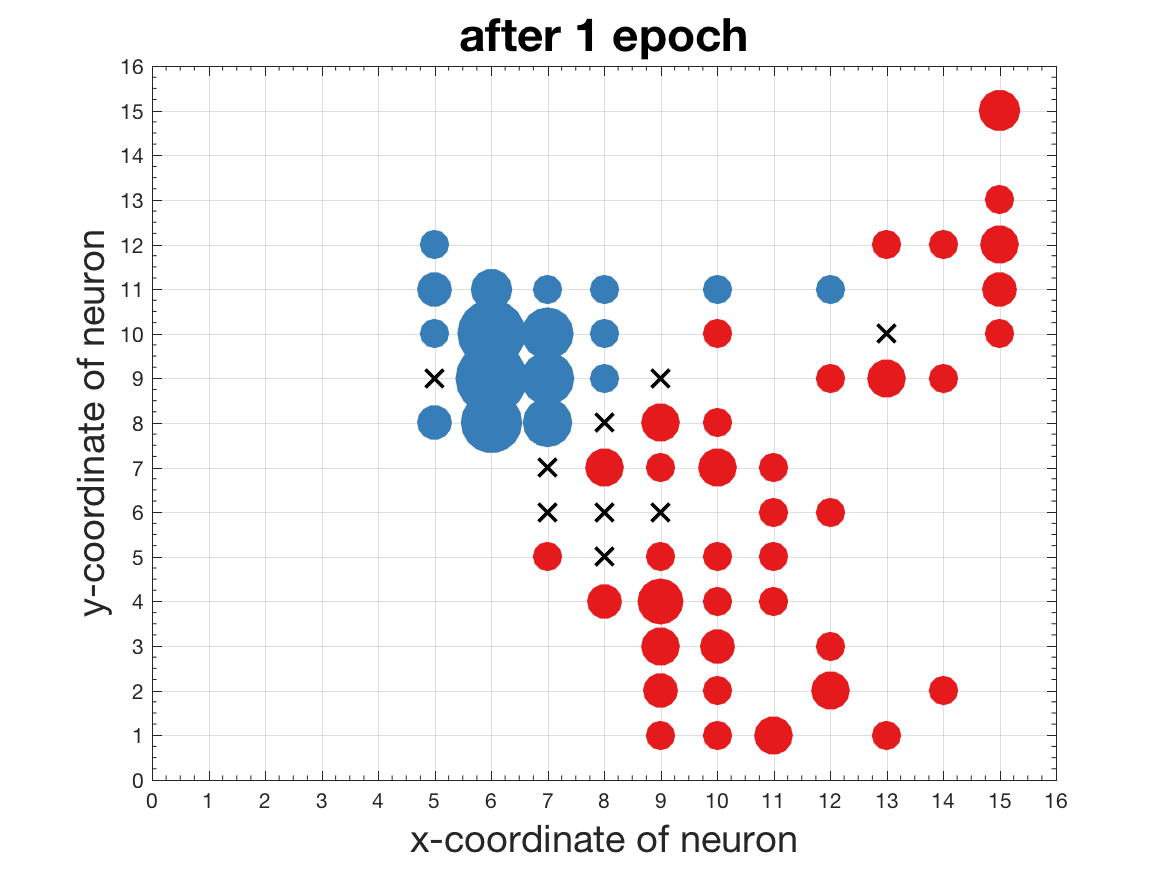
\includegraphics[width=.32\textwidth]{exp_kp_ram_norm_1.png}
    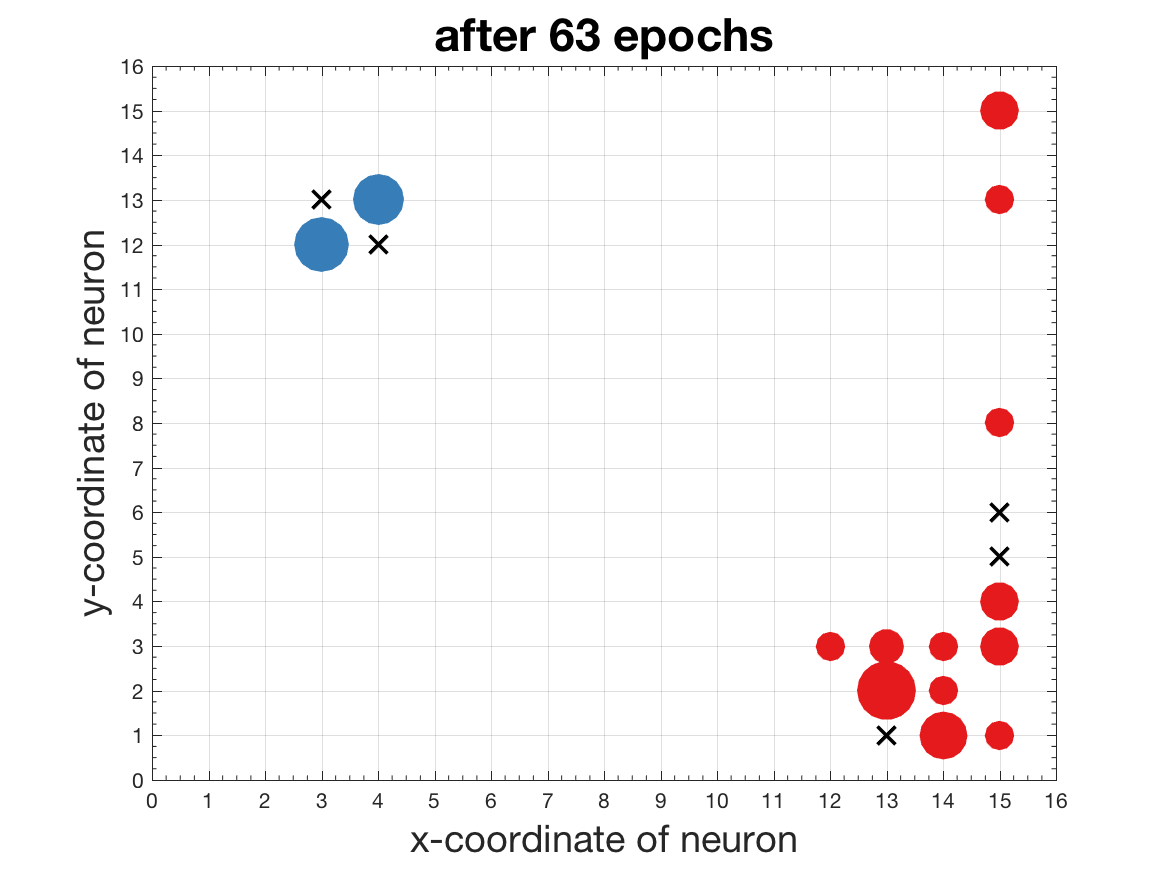
\includegraphics[width=.32\textwidth]{exp_kp_ram_norm_63.png}
    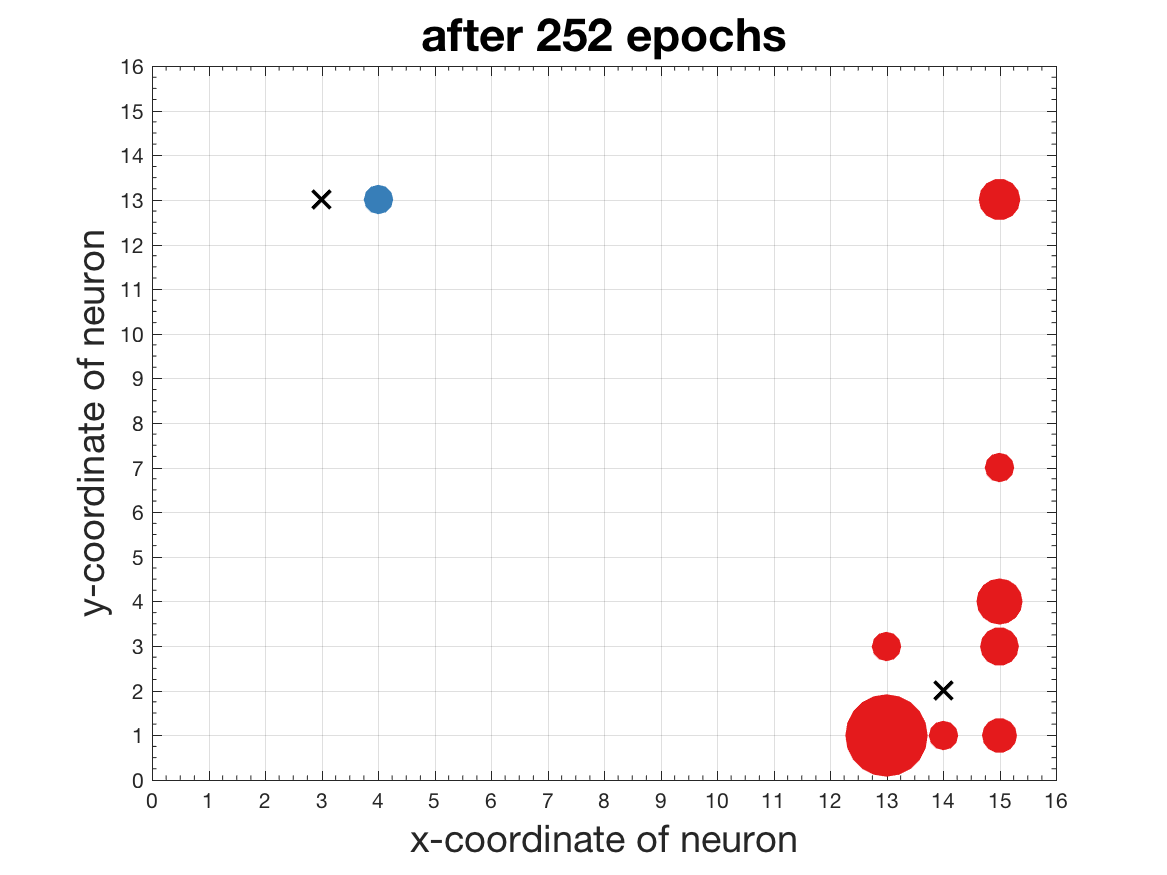
\includegraphics[width=.32\textwidth]{exp_kp_ram_norm_252.png}
    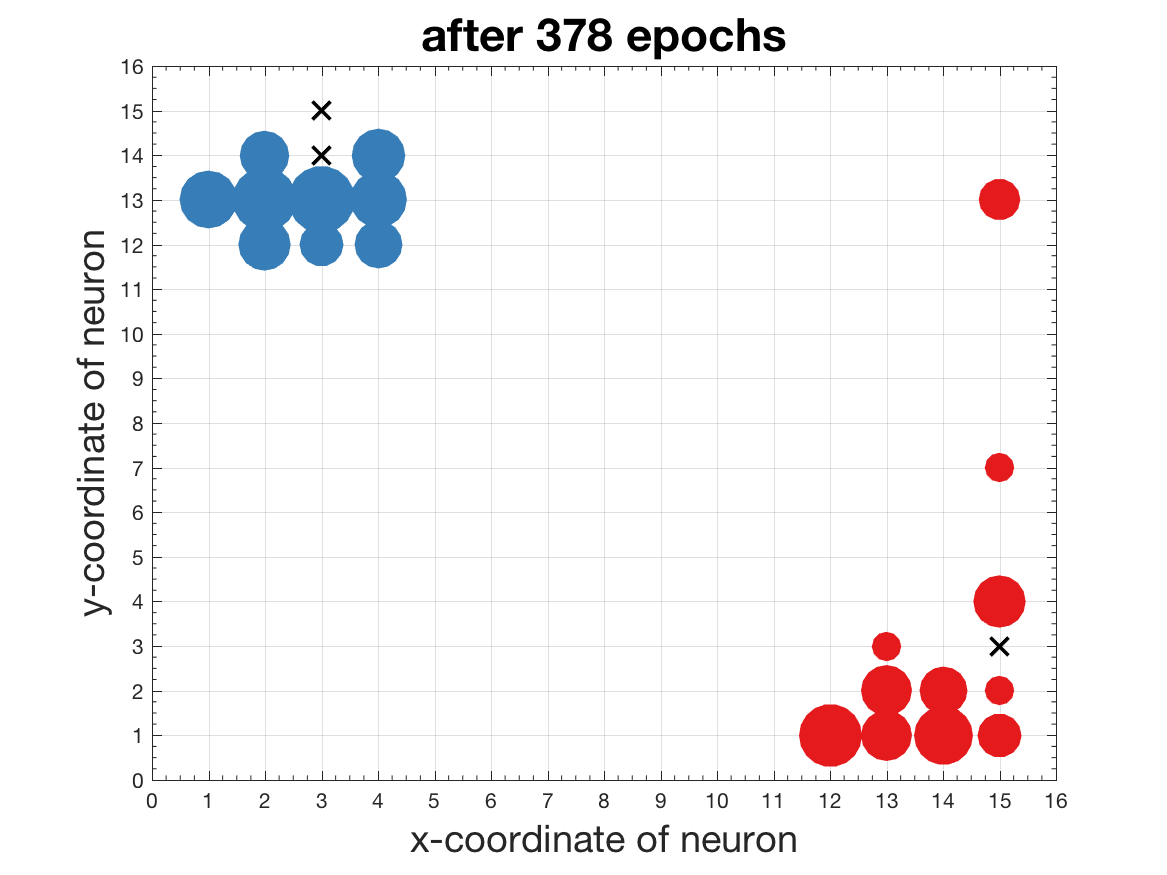
\includegraphics[width=.32\textwidth]{exp_kp_ram_norm_378.png}
    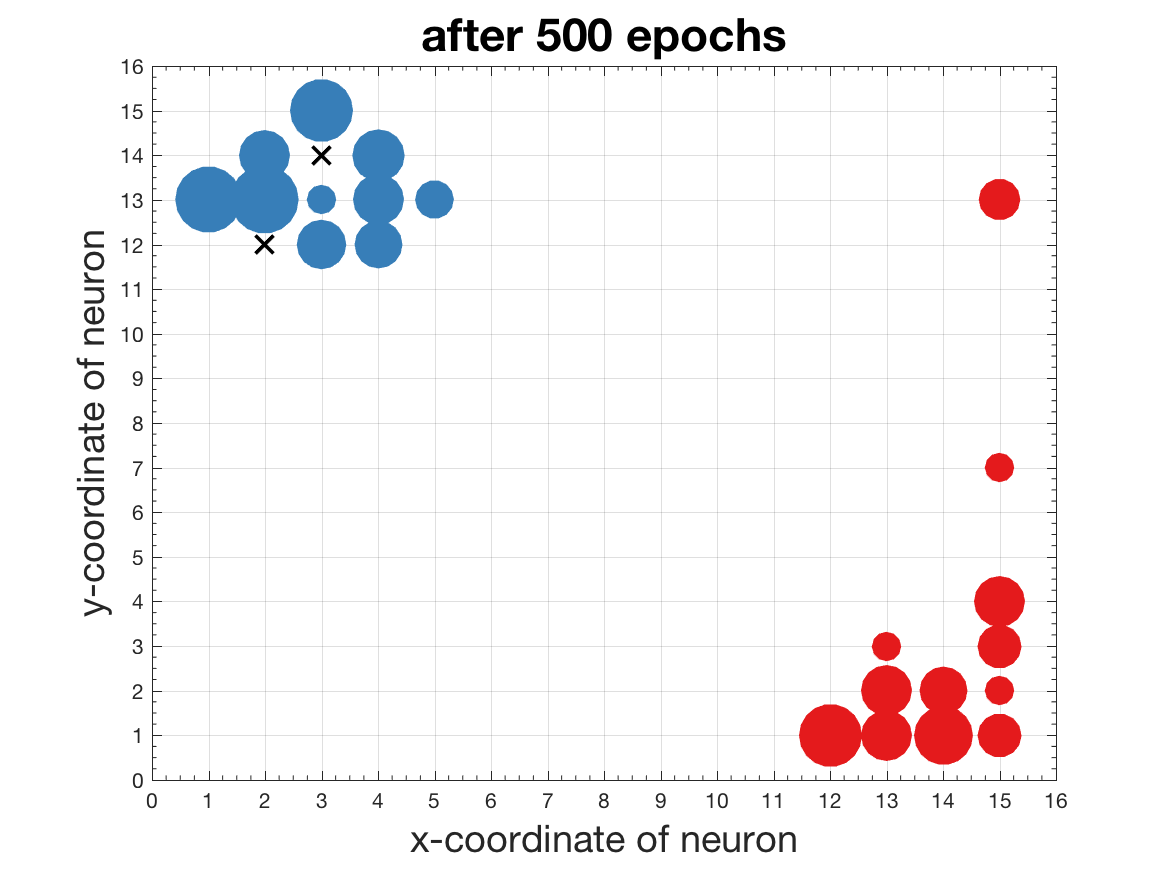
\includegraphics[width=.32\textwidth]{exp_kp_ram_norm_500.png}
    \caption{Formování sémantické mapy.}
    \label{fig:mapform}
\end{figure}

\begin{figure}[htp]
    \centering
    
    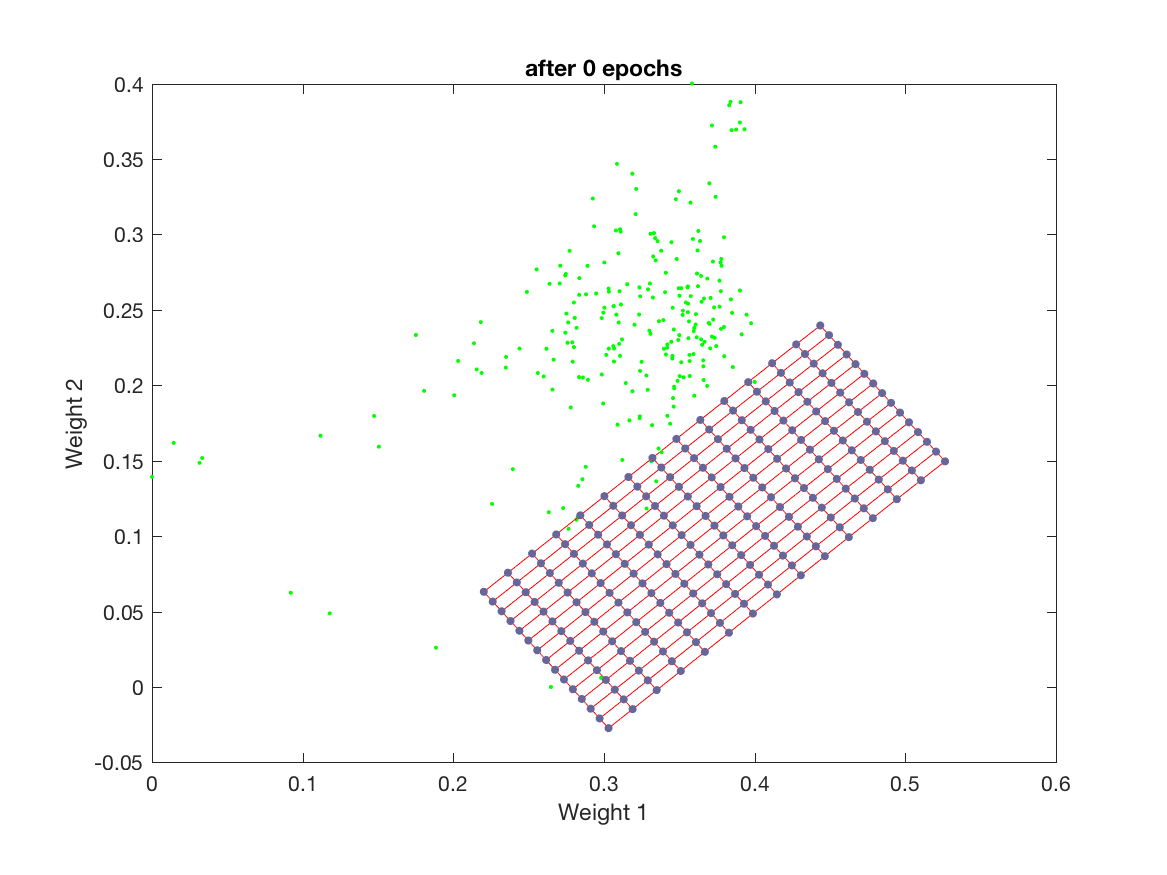
\includegraphics[width=.32\textwidth]{exp_kp_ram_pos0.png}
    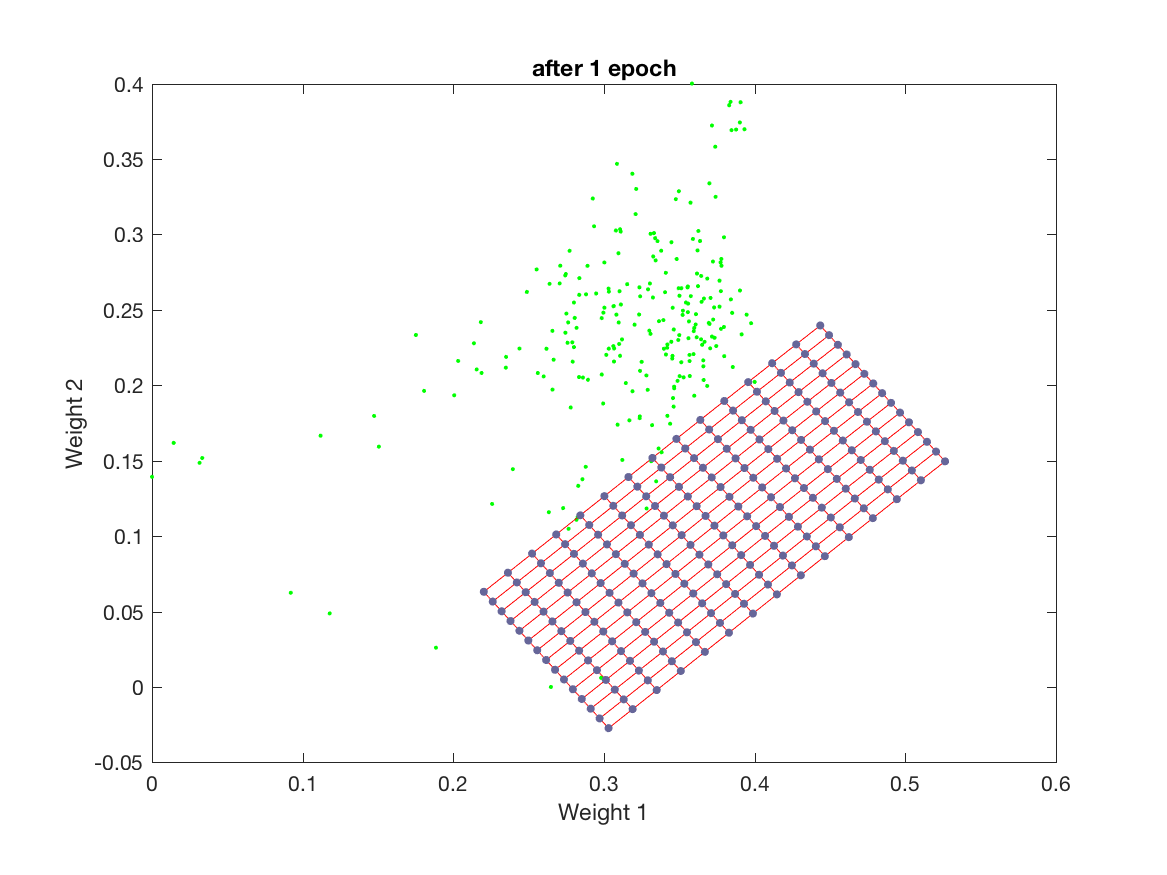
\includegraphics[width=.32\textwidth]{exp_kp_ram_pos1.png}
    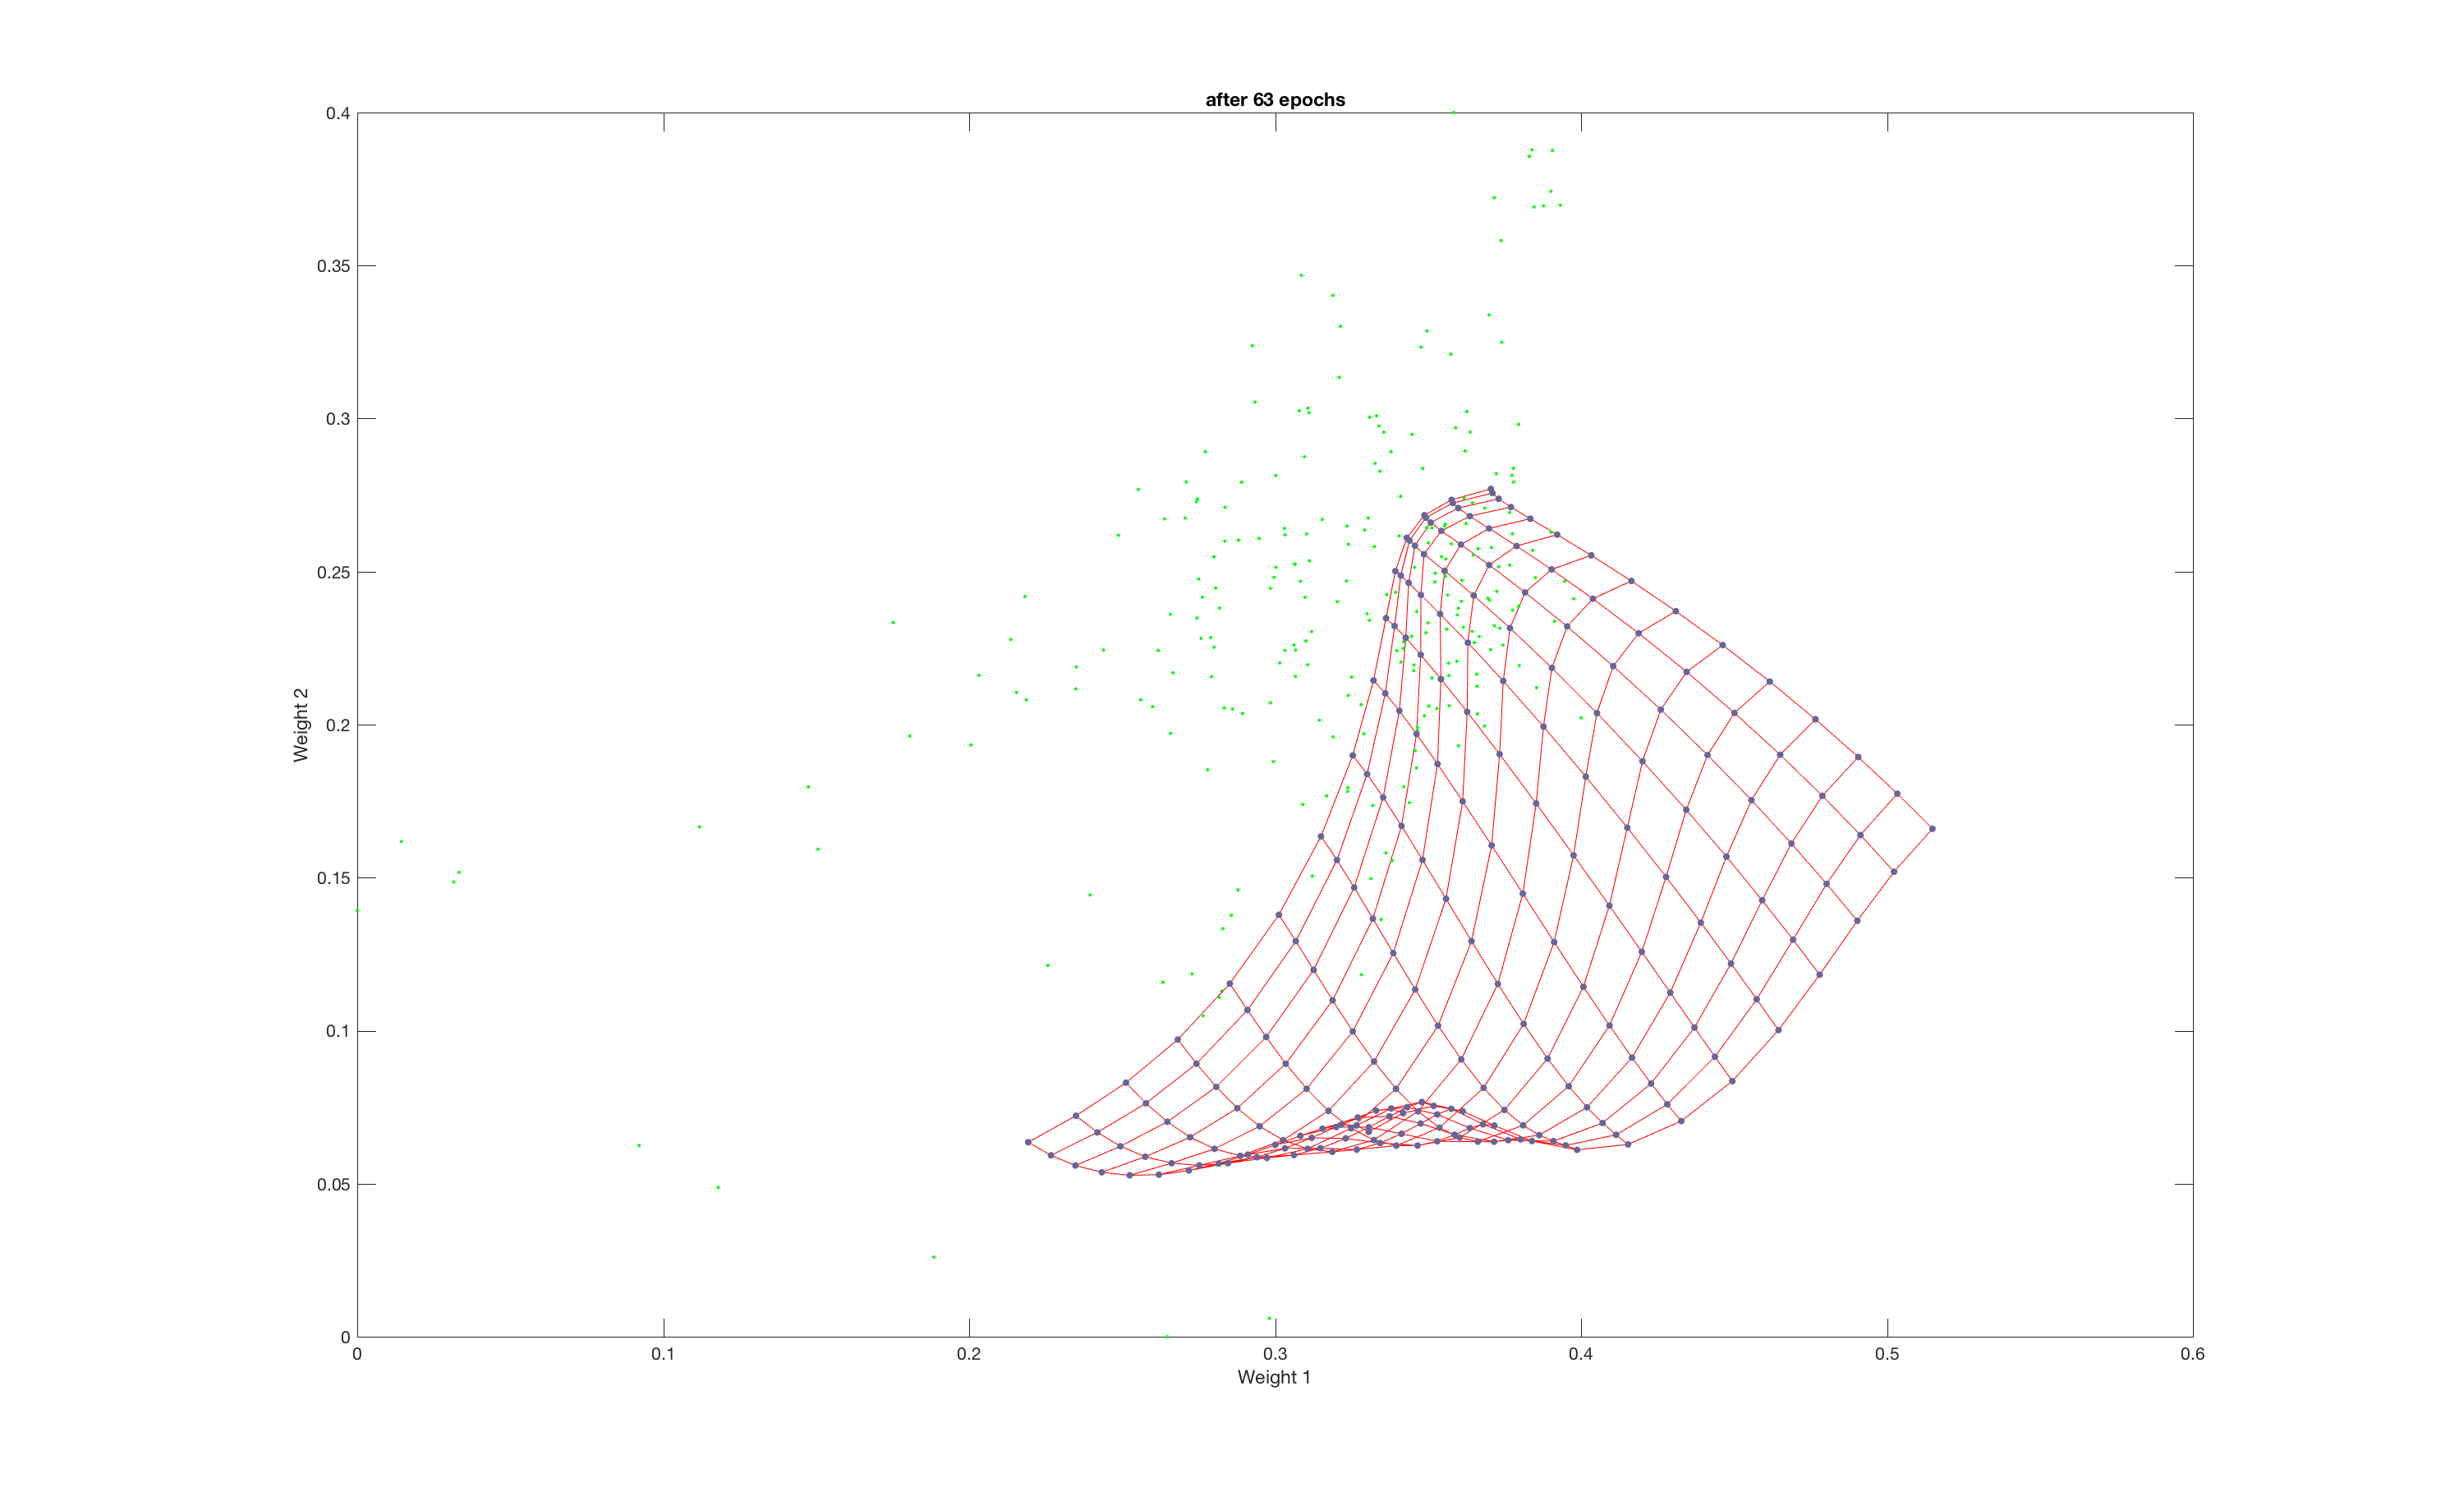
\includegraphics[width=.32\textwidth]{exp_kp_ram_pos63.png}
        \includegraphics[width=.32\textwidth]{exp_kp_ram_pos252.png}
    \includegraphics[width=.32\textwidth]{exp_kp_ram_pos378.png}
    \includegraphics[width=.32\textwidth]{exp_kp_ram_pos500.png}
    \caption{Pozice neuronů pro první dvě dimenze}
    \label{fig:mappos}
\end{figure}


\section{Testování reprezentace}
Reprezentace původních skladeb, tedy příslušných $90$ atributů vzniklo netriviální extrakcí z akustických vlastností původních objektů. Tento přístup zabraňuje interpretovat výsledné shluky podle společných vlastností odvozených pouze na základě konkrétních hodnot atributů. Lepším přístupem je interpretovat shluky podle původních objektů, tedy skladeb, což je ovšem záležitost, kterou má v popisu činnosti expert domény.

V této části proto nepůjde primárně o interpretaci výsledných shluků, nýbrž o nalezení nějaké struktury. Výsledkem této sekce by tak mělo být ujištění, že zvolené metody jsou schopné najít strukturu v kolekcích reprezentací hudebních skladeb v kontextu zvolené sémantiky. Proto budou voleny takové datasety u kterých se struktura předpokládá.



\subsection{Interpret jako sémantický kontext}
\subsubsection*{Katy Perry a Ramones}
Jako první sémantika učení byla zvolena podle interpreta skladby. První zkoumaný dataset byl již představený --KatyRamDataset (\ref{app:KatyRamDataset}), který obsahuje skladby zpěvačky Katy Perry a kapely Ramones. Výsledky  experimentu (exp. \ref{exp:kp_ram}) jsou v podobě dvou sémantických map (obr. \ref{fig:kp_ram_res}). První mapa (obr. \ref{fig:kp_ram_som}) představuje natrénovanou samoorganizující mapu, zatímco druhá mapa (obr. \ref{fig:kp_ram_crsom}) pochází ze skryté vrstvy natrénované samoorganizující mapy se zahrnutým sémantickým kontextem.

	SOM při učení nebere v úvahu třídy vstupních vektorů a výsledná sémantická mapa vizualizuje pouze povahu vstupního prostoru. Podle této vizualizace (obr. \ref{fig:kp_ram_som}) lze konstatovat celkovou rozdílnost vektorů spadající do různých tříd.
	
	Oproti tomu CRSOM sémantický kontext zahrnuje do procesu učení explicitně a z příslušné sémantické mapy (obr. \ref{fig:kp_ram_crsom}) lze extrahovat rozdílné znalosti. Síť vytvořila dva koncentrované shluky v rozích mapy, což svědčí o dobré oddělitelnosti těchto dvou tříd. Konfliky v horním shluku (např neuron [3;14])implikuje podobné reprezentace pro skladby s rozdílnými sémantikami. Tato podobnost je již zřejmá z mapy SOM -- např. neuronem [2;9].  TODO více epoch. Neuron [15;13] představuje shluk odlehlých hodnot. Po prozkoumání objektů, které přísluší tomuto neuronu se ukázalo, že tyto nahrávky neobsahují hudbu, nýbrž se jedná o mluvené slovo Katy Perry a poskytovatel dat ho mylně zařadil mezi skladby.

\begin{figure}
\centering
\begin{subfigure}{.5\textwidth}
  \centering
  \includegraphics[width=.99\linewidth]{exp_kp_ram_som.png}
  \caption{SOM}
  \label{fig:kp_ram_som}
\end{subfigure}%
\begin{subfigure}{.5\textwidth}
  \centering
  \includegraphics[width=.99\linewidth]{exp_kp_ram_crsom.png}
  \caption{CRSOM}
  \label{fig:kp_ram_crsom}
\end{subfigure}
\caption{Katy Perry a Ramones (exp. \ref{exp:kp_ram})}
\label{fig:kp_ram_res}
\end{figure}


\subsubsection*{The Offspring a Sex Pistols}
Další dataset se skládá z diskografie kapel Sex Pistols a The Offspring. Mapa SOM (obr. \ref{fig:sexp_off_som}) zobrazuje větší promíchanost objektů v prostoru, než se tomu jednalo u  předchozího experimentu, což svědčí o větší podobnosti hudebních znaků těchto dvou kapel. I přes tento fakt jsou data dobře oddělitelné podle této sémantiky (obr. \ref{fig:sexp_off_crsom}). Výsledná mapa dokonce neobsahuje žádné konflikty, což lze přisoudit delšímu učení (exp. \ref{exp:sexp-off}), než v předchozím případě.


\begin{figure}
\centering
\begin{subfigure}{.5\textwidth}
  \centering
  \includegraphics[width=.99\linewidth]{exp_sexp_off_som.png}
  \caption{SOM}
  \label{fig:sexp_off_som}
\end{subfigure}%
\begin{subfigure}{.5\textwidth}
  \centering
  \includegraphics[width=.99\linewidth]{exp_sexp_off_crsom.png}
  \caption{CRSOM}
  \label{fig:sub2}
\end{subfigure}
\caption{Sex Pistols a The Offspring (exp. \ref{exp:sexp-off})}
\label{fig:sexp_off_crsom}
\end{figure}

\subsubsection*{David Bowie, Elvis Presley a AC/DC}
Další zkoumaný dataset obsahuje skladby následujících interpretů: David Bowie, Elvis Presley a AC/DC. I zde se jedná o dobře rozlišitelné interprety o čemž svědčí výsledky experimentů (obr. \ref{fig:db_ep_acdc}).


\begin{figure}
\centering
\begin{subfigure}{.5\textwidth}
  \centering
  \includegraphics[width=.99\linewidth]{exp_db_ep_acdc_som.png}
  \caption{SOM}
  \label{fig:sub1}
\end{subfigure}%
\begin{subfigure}{.5\textwidth}
  \centering
  \includegraphics[width=.99\linewidth]{exp_db_ep_acdc_crsom.png}
  \caption{CRSOM}
  \label{fig:sub2}
\end{subfigure}
\caption{David Bowie, Elvis Presley a AC/DC (exp. \ref{exp:db-ep-acdc})}
\label{fig:db_ep_acdc}
\end{figure}
% db_stones_acdc_ep=1000_norm=4_size=1.00_LR2=0.10_.mat

\subsubsection*{Metallica, Maddona a Louis Armstrong}
Poslední dataset s daty rozdělenými do tříd podle interpretů je met-mad-la-dataset (\ref{d:met_mad_la}). Tak jako ve všech předchozích případech, i zde CRSOM síť dokázala sformovat dobře ucelené shluky podle dané sémantiky (obr. \ref{fig:metmadlacrsom}).

\begin{figure}
\centering
\begin{subfigure}{.5\textwidth}
  \centering
  \includegraphics[width=.99\linewidth]{exp_met_mad_la_som.png}
  \caption{SOM}
  \label{fig:sub1}
\end{subfigure}%
\begin{subfigure}{.5\textwidth}
  \centering
  \includegraphics[width=.99\linewidth]{exp_met_mad_la_crsom.png}
  \caption{CRSOM}
  \label{fig:metmadlacrsom}
\end{subfigure}
\caption{Metallica, Maddona a Louis Armstrong (exp. \ref{exp:met-mad-la})}
\label{fig:top}
\end{figure}
%met_mad_la_ep=2500_norm=4_size=1.00_LR2=0.05_.mat


Pro představu, jak vypadá sémantická mapa, ze které nelze extrahovat žádnou strukturu dat, byla vytvořena náhodná sémantika pro dataset met-mad-la. Sémantika byla vytvořena náhodným proházením tříd objektů. Sítě SOM a CRSOM byly učeny  se stejnými parametry jako v předchozím v případě. Výsledky tohoto experimentu jsou na obrázku \ref{fig:metmadlarandom}.

\begin{figure}
\centering
\begin{subfigure}{.5\textwidth}
  \centering
  \includegraphics[width=.99\linewidth]{exp_met_mad_la_random_som.png}
  \caption{SOM}
  \label{fig:sub1}
\end{subfigure}%
\begin{subfigure}{.5\textwidth}
  \centering
  \includegraphics[width=.99\linewidth]{exp_met_mad_la_random_crsom.png}
  \caption{CRSOM}
  \label{fig:sub2}
\end{subfigure}
\caption{Dataset s náhodnou sémantikou (exp \ref{exp:met-mad-la-random})}
\label{fig:metmadlarandom}
\end{figure}

% off-sexp_ep=2500_norm=4_size=1.00_LR2=0.10_.mat


\subsection{Rok vzniku jako sémantický kontext}
Další zkoumaná sémantika je rok vzniku sladby. Pro tento účel byly vytvořeny dva datasety 60-vs-70-dataset (\ref{app:60vs70dataset}) a 70-vs-10-dataset \ref{app:70vs10dataset}. V tomto případě se jedná o obrovské datasety, potažmo sítě, které bylo nutné učit po velký počet epoch, v řádech tisíců. Předpoklad, že pomocí CRSOM map bude možné extrahovat strukturu kolekcí, se naplnil a v obou případech je možné určit několik shluků pro jednotlivé sémantiky. Více shluků v rámci jedné třídy svědčí o rozdílnosti skladeb v jedné sémantice, což je další předpokládaný závěr.


\begin{figure}
\centering
\begin{subfigure}{.5\textwidth}
  \centering
  \includegraphics[width=.99\linewidth]{exp_60s70s_som.png}
  \caption{SOM}
  \label{fig:sub1}
\end{subfigure}%
\begin{subfigure}{.5\textwidth}
  \centering
  \includegraphics[width=.99\linewidth]{exp_60s70s_crsom.png}
  \caption{CRSOM}
  \label{fig:sub2}
\end{subfigure}
\caption{Skladby z 1960 a 1970 (exp. \ref{exp:60-vs-70}) }
\label{fig:top}
\end{figure}

\begin{figure}
\centering
\begin{subfigure}{.5\textwidth}
  \centering
  \includegraphics[width=.99\linewidth]{exp_70s10s_som.png}
  \caption{SOM}
  \label{fig:sub1}
\end{subfigure}%
\begin{subfigure}{.5\textwidth}
  \centering
  \includegraphics[width=.99\linewidth]{exp_70s10s_crsom.png}
  \caption{CRSOM}
  \label{fig:sub2}
\end{subfigure}
\caption{Skladby z 1970 a 2010 (exp. \ref{exp:70-vs-10})}
\label{fig:top}
\end{figure}

méně konfliktů (rozdílná hudba)






\section{Hledání struktur}


\subsection{Posluchačská historie jako sémantický kontext}
V této sekci je použita historie přehrávání náhodného uživatele. Máme k dispozici přehrané skladby a k nim počet přehrání. Pro vytvoření tříd byla zvolena denormalizace do tří tříd:

\begin{itemize}
\item třída A: $1$ přehrání,
\item třída B: $2-4$ přehrání,
\item třída C: $\geq5$ přehrání.
\end{itemize}

Předpokladem je, že počty přehrání odrážejí uživatelskou oblíbenost skladby a tato oblíbenost je stanovena hudebními znaky. Výsledky učení v kontextu takto zvolené sémantiky jsou na obr. \ref{fig:user1}. Ze sémantické mapy SOM (obr. \ref{fig:usersom}) nelze odvodit žádné pravidelnosti. CRSOM mapa (obr. \ref{fig:usercrsom}) utvořila několik shluků, ale žádný z nich není koncentrovaný a homogenní. To je možné dát za vinu špatnému rozdělení do tříd, které nenese žádné pravidelnosti.

První problém je se skladbami, které mají jediné přehrání a není u nich jasné, jestli se jedná o konečný počet. Ve shluku $1$ jsou koncentrované skladby všech tříd, což znamená, že i přes své rozdílné sémantiky nebyly učením odděleny, což implikuje  velmi podobné reprezentace. Za stanovených předpokladů je možné skladby s jedním přehráním ve shluku 1 interpretovat jako nově objevené a jediný počet přehrání je pouze dočasný, protože sdílejí hudbení znaky i s ostatními třídami.

Další problém je uměle stanovená hranice pěti přehrání, která představuje vysoce oblíbenou skladbu. Shluky $2$ a $3$ obsahují pouze hudbu třídy B a C a je možné je označit jako oblíbené s potenciálem dalších přehrávání.

\begin{figure}
\centering
\begin{subfigure}{.5\textwidth}
  \centering
  \includegraphics[width=.99\linewidth]{exp_user_som.png}
  \caption{SOM mapa}
  \label{fig:usersom}
\end{subfigure}%
\begin{subfigure}{.5\textwidth}
  \centering
  \includegraphics[width=.99\linewidth]{exp_user_crsom_ann.png}
  \caption{anotovaná CRSOM mapa}
  \label{fig:usercrsom}
\end{subfigure}
\caption{Posluchačská historie $3$ třídy (exp. \ref{ex:user1})}
\label{fig:user1}
\end{figure}


V dalším experimentu byla prozkoumána rozdílná sémantika pro stejná data:

\begin{itemize}
\item třída X: $1$ přehrání,
\item třída Y: $\geq2$ přehrání.
\end{itemize}

Výsledky jsou k vidění na obr. \ref{fig:user2}. Narozdíl od předchozí sémantiky, takto zvolené třídy vytvářejí dobře oddělitelné shluky \ref{fig:user2crsom}. Sklady spadající do třídy Y vytváří nepříliš koncentrovaný shluk, což svědčí o hudební rozmanitosti těchto skladeb. Dva konfliky (neurony $[10;5]$ a $[11;6]$) byly BMU pro některé skladby s jedním přehráním. Pro podobnost reprezentací se skaldbami z třídy Y lze předpokládat další přehrávání těchto skladeb.

Kategorie X vytvořila několik shluků, které učení CRSOM nepodařilo sloučit, což implikuje vysoké rozdílnosti v reprezentacích v rámci jedné třídy. Tento fakt je možné vysvětlit již zmíněným nejasným významem jednoho přehrání, který se dá iterpretovat jako neoblíbená hudba, nebo jako nová hudba.  





\begin{figure}
\centering
\begin{subfigure}{.5\textwidth}
  \centering
  \includegraphics[width=.99\linewidth]{exp_user2_som.png}
  \caption{SOM}
  \label{fig:sub1}
\end{subfigure}%
\begin{subfigure}{.5\textwidth}
  \centering
  \includegraphics[width=.99\linewidth]{exp_user2_crsom.png}
  \caption{CRSOM}
  \label{fig:user2crsom}
\end{subfigure}
\caption{Posluchačská historie s rozdílnou sémantikou (exp. \ref{ex:user2})}
\label{fig:user2}
\end{figure}






\subsection{Oblíbenost jako sémantický kontext}\label{sec:hotness}
V této sekci budou zkoumány struktury hudebních kolekcí se sémantikou podle oblíbenosti. V představení dostupných dat bylo zmíněno, že API poskytuje míru současné oblíbenosti skladby atributem \textit{hotttnesss}. Tato hodnota je odvozena z mnoha zdrojů jako jsou zmínky na webu, hudební recenze, dále podle počtů stažení a přehrání \cite{hotttnesss}.

Protože je atribut hotttnesss desetinné číslo, bylo nutné ho denormalizovat do dvou tříd (Fail a Hot). Konkrétní rozdělení je názorně předvedeno v krabicovém diagramu na obrázku \ref{fig:boxplot}.

Z výsledků (obr. \ref{fig:hotfail}) lze usoudit, že podle této sémantiky jsou data dobře oddělitelná. Mapa neobsahuje koncentrované shluky, což svědčí o tom, že v obou třídách se vyskytují skladby z různých hudebních odvětví.



\begin{figure}[htbp]
\begin{center}
	\includegraphics[scale=0.25]{exp_boxplot.png}
\caption{Krabicový diagram pro hotttnesss.}
\label{fig:boxplot}
\end{center}
\end{figure}

  

\begin{figure}
\centering
\begin{subfigure}{.5\textwidth}
  \centering
  \includegraphics[width=.99\linewidth]{exp_trend_fail2_som.png}
  \caption{SOM}
  \label{fig:sub1}
\end{subfigure}%
\begin{subfigure}{.5\textwidth}
  \centering
  \includegraphics[width=.99\linewidth]{exp_trend_fail2_crsom.png}
  \caption{CRSOM}
  \label{fig:sub2}
\end{subfigure}
\caption{Oblíbenost skladby (exp. \ref{ex:hotfail})}
\label{fig:hotfail}
\end{figure}



% -------------------------------------- Využití ---------------------------------------------------------------------------------------------------------------------------------------------------------------
\chapter{Využití}

Využítí je poslední částí KDD. V této kapitole budou představeny dvě možnosti, jak využít získané výstupy z dataminingových metod. Obě možnosti představují koncepty teoreticky využitelného softwarového výrobeku.

\section{Mapa hudebního vkusu}


\section{Predikce úspěšnosti pro novou skladbu}
Tento koncept byl inspirován experimenty v sekci \ref{sec:hotness}. 


\begin{conclusion}
	co se všechno udělalo v této práci (mělo by sedět s cílem)
	+ nějaké další návrhy
	
	\section{Přínosy}
	
	\section{Možná rozšíření}
\end{conclusion}

\bibliographystyle{csn690}
\bibliography{mybibliographyfile}

\appendix

\chapter{Seznam použitých zkratek}
% \printglossaries
\begin{description}
	\item[KDD] \dots
	\item[CPU] \dots
\end{description}

\chapter{Definice pojmů}


\chapter{Obsah přiloženého CD}

%upravte podle skutecnosti

\begin{figure}
	\dirtree{%
		.1 readme.txt\DTcomment{stručný popis obsahu CD}.
		.1 exe\DTcomment{adresář se spustitelnou formou implementace}.
		.1 src.
		.2 impl\DTcomment{zdrojové kódy implementace}.
		.2 thesis\DTcomment{zdrojová forma práce ve formátu \LaTeX{}}.
		.1 text\DTcomment{text práce}.
		.2 thesis.pdf\DTcomment{text práce ve formátu PDF}.
		.2 thesis.ps\DTcomment{text práce ve formátu PS}.
	}
\end{figure}


\chapter{Datasety}

\section{Interpret jako sémantika}

\subsection{Katy Perry a Ramones (katy-ram-dataset)}\label{sec:katy-ram-dataset}

celkový počet záznamů
Katy Perry 50\%
Ramones 50\%

\subsection{The Offspring a Sex (off-sexp-dataset)}\label{sec:off-sexp-dataset}

\subsection{David Bowie, Elvis Presley a AC/DC (dp-ep-acdc-dataset)}\label{sec:dp-ep-acdc-dataset}

\subsection{Metallica, Maddona a Louis Armstrong (met-mad-la-dataset)}\label{sec:met-mad-la-dataset}

\subsection{Metallica, Maddona a Louis Armstrong náhodný (met-mad-la-random-dataset)}\label{sec:met-mad-la-random-dataset}

\section{Rok vzniku skladby jako sémantika}

\subsection{Skladby z roku 1960 a 1970 (60-vs-70-dataset)}\label{sec:60-vs-70-dataset}

\subsection{Skladby z roku 1970 a 2010 (70-vs-10-dataset)}\label{sec:70-vs-10-dataset}

\section{Počet přehrání jako sémantika}

\subsection{Počty přehrání rozdělené do třech kategorií (user-3class-dataset)}\label{sec:user-3class-dataset}
\subsection{Počty přehrání rozdělené do dvou kategorií (user-2class-dataset)}\label{sec:user-2class-dataset}

\section{Oblíbenost jako sémantika}

\subsection{Hot a fail skladby (hot-fail-dataset)}\label{sec:hot-fail-dataset}

\chapter{Protokoly experimentů}
\section{Experiment}

- datset
- SOM
- CRSOM
- ploterror?

\subsection{Experiment}\label{exp:kp_ram}
\subsubsection*{SOM}
\dots
\subsubsection*{CRSOM}
\dots

\section{David Bowie, Elvis Presley a AC/DC (db-ep-acdc-dataset)}\label{app:db-ep-acdc-dataset}
\subsection{Experiment}\label{exp:db-ep-acdc}


\section{Metallica, Maddona a Louis Armstrong (met-mad-la-dataset)}\label{app:met-mad-la}
\subsection{Experiment}\label{exp:met-mad-la}

\section{Sex Pistols a The Offspring (sexp-off-dataset)}\label{app:sexp-off}
\subsection{Experiment}\label{exp:sexp-off}


\section{Skladby z roku 1960 a 1970 (60-vs-70-dataset)}\label{app:60vs70dataset}
\subsection{Experiment}\label{exp:60-vs-70}


\section{Skladby z roku 1970 a 2010 (70-vs-10-dataset)}\label{app:70vs10dataset}
\subsection{Experiment}\label{exp:70-vs-10}


\begin{figure}
\centering

\begin{subfigure}{.5\textwidth}
  \centering
  \includegraphics[width=1\linewidth]{exp_sexp_off_som.png}
  \caption{SOM}
  \label{fig:sub1}
\end{subfigure}%
\begin{subfigure}{.5\textwidth}
  \centering
  \includegraphics[width=1\linewidth]{exp_sexp_off_som.png}
  \caption{SOM}
  \label{fig:sub1}
\end{subfigure}%



\begin{subfigure}{.5\textwidth}
  \centering
  \includegraphics[width=1\linewidth]{exp_sexp_off_som.png}
  \caption{SOM}
  \label{fig:sub1}
\end{subfigure}%
\begin{subfigure}{.5\textwidth}
  \centering
  \includegraphics[width=1\linewidth]{exp_sexp_off_som.png}
  \caption{SOM}
  \label{fig:sub1}
\end{subfigure}%


\caption{Sex Pistols a The Offspring (exp. \ref{exp:sexp-off})}
\label{fig:top}


\end{figure}

% % % % % % % % % % % % % % % % % % % % % % % % % % % % 
% % Tuto kapitolu z výsledné práce ODSTRAŇTE.
% % % % % % % % % % % % % % % % % % % % % % % % % % % % 
% 
% \chapter{Návod k~použití této šablony}
% 
% Tento dokument slouží jako základ pro napsání závěrečné práce na Fakultě informačních technologií ČVUT v~Praze.
% 
% \section{Výběr základu}
% 
% Vyberte si šablonu podle druhu práce (bakalářská, diplomová), jazyka (čeština, angličtina) a kódování (ASCII, \mbox{UTF-8}, \mbox{ISO-8859-2} neboli latin2 a nebo \mbox{Windows-1250}). 
% 
% V~české variantě naleznete šablony v~souborech pojmenovaných ve formátu práce\_kódování.tex. Typ může být:
% \begin{description}
% 	\item[BP] bakalářská práce,
% 	\item[DP] diplomová (magisterská) práce.
% \end{description}
% Kódování, ve kterém chcete psát, může být:
% \begin{description}
% 	\item[UTF-8] kódování Unicode,
% 	\item[ISO-8859-2] latin2,
% 	\item[Windows-1250] znaková sada 1250 Windows.
% \end{description}
% V~případě nejistoty ohledně kódování doporučujeme následující postup:
% \begin{enumerate}
% 	\item Otevřete šablony pro kódování UTF-8 v~editoru prostého textu, který chcete pro psaní práce použít -- pokud můžete texty s~diakritikou normálně přečíst, použijte tuto šablonu.
% 	\item V~opačném případě postupujte dále podle toho, jaký operační systém používáte:
% 	\begin{itemize}
% 		\item v~případě Windows použijte šablonu pro kódování \mbox{Windows-1250},
% 		\item jinak zkuste použít šablonu pro kódování \mbox{ISO-8859-2}.
% 	\end{itemize}
% \end{enumerate}
% 
% 
% V~anglické variantě jsou šablony pojmenované podle typu práce, možnosti jsou:
% \begin{description}
% 	\item[bachelors] bakalářská práce,
% 	\item[masters] diplomová (magisterská) práce.
% \end{description}
% 
% \section{Použití šablony}
% 
% Šablona je určena pro zpracování systémem \LaTeXe{}. Text je možné psát v~textovém editoru jako prostý text, lze však také využít specializovaný editor pro \LaTeX{}, např. Kile.
% 
% Pro získání tisknutelného výstupu z~takto vytvořeného souboru použijte příkaz \verb|pdflatex|, kterému předáte cestu k~souboru jako parametr. Vhodný editor pro \LaTeX{} toto udělá za Vás. \verb|pdfcslatex| ani \verb|cslatex| \emph{nebudou} s~těmito šablonami fungovat.
% 
% Více informací o~použití systému \LaTeX{} najdete např. v~\cite{wikilatex}.
% 
% \subsection{Typografie}
% 
% Při psaní dodržujte typografické konvence zvoleného jazyka. České \uv{uvozovky} zapisujte použitím příkazu \verb|\uv|, kterému v~parametru předáte text, jenž má být v~uvozovkách. Anglické otevírací uvozovky se v~\LaTeX{}u zadávají jako dva zpětné apostrofy, uzavírací uvozovky jako dva apostrofy. Často chybně uváděný symbol "{} (palce) nemá s~uvozovkami nic společného.
% 
% Dále je třeba zabránit zalomení řádky mezi některými slovy, v~češtině např. za jednopísmennými předložkami a spojkami (vyjma \uv{a}). To docílíte vložením pružné nezalomitelné mezery -- znakem \texttt{\textasciitilde}. V~tomto případě to není třeba dělat ručně, lze použít program \verb|vlna|.
% 
% Více o~typografii viz \cite{kobltypo}.
% 
% \subsection{Obrázky}
% 
% Pro umožnění vkládání obrázků je vhodné použít balíček \verb|graphicx|, samotné vložení se provede příkazem \verb|\includegraphics|. Takto je možné vkládat obrázky ve formátu PDF, PNG a JPEG jestliže používáte pdf\LaTeX{} nebo ve formátu EPS jestliže používáte \LaTeX{}. Doporučujeme preferovat vektorové obrázky před rastrovými (vyjma fotografií).
% 
% \subsubsection{Získání vhodného formátu}
% 
% Pro získání vektorových formátů PDF nebo EPS z~jiných lze použít některý z~vektorových grafických editorů. Pro převod rastrového obrázku na vektorový lze použít rasterizaci, kterou mnohé editory zvládají (např. Inkscape). Pro konverze lze použít též nástroje pro dávkové zpracování běžně dodávané s~\LaTeX{}em, např. \verb|epstopdf|.
% 
% \subsubsection{Plovoucí prostředí}
% 
% Příkazem \verb|\includegraphics| lze obrázky vkládat přímo, doporučujeme však použít plovoucí prostředí, konkrétně \verb|figure|. Například obrázek \ref{fig:float} byl vložen tímto způsobem. Vůbec přitom nevadí, když je obrázek umístěn jinde, než bylo původně zamýšleno -- je tomu tak hlavně kvůli dodržení typografických konvencí. Namísto vynucování konkrétní pozice obrázku doporučujeme používat odkazování z~textu (dvojice příkazů \verb|\label| a \verb|\ref|).
% 
% \begin{figure}\centering
% 	\includegraphics[width=0.5\textwidth, angle=30]{cvut-logo-bw}
% 	\caption[Příklad obrázku]{Ukázkový obrázek v~plovoucím prostředí}\label{fig:float}
% \end{figure}
% 
% \subsubsection{Verze obrázků}
% 
% % Gnuplot BW i barevně
% Může se hodit mít více verzí stejného obrázku, např. pro barevný či černobílý tisk a nebo pro prezentaci. S~pomocí některých nástrojů na generování grafiky je to snadné.
% 
% Máte-li například graf vytvořený v programu Gnuplot, můžete jeho černobílou variantu (viz obr. \ref{fig:gnuplot-bw}) vytvořit parametrem \verb|monochrome dashed| příkazu \verb|set term|. Barevnou variantu (viz obr. \ref{fig:gnuplot-col}) vhodnou na prezentace lze vytvořit parametrem \verb|colour solid|.
% 
% \begin{figure}\centering
% 	\includegraphics{gnuplot-bw}
% 	\caption{Černobílá varianta obrázku generovaného programem Gnuplot}\label{fig:gnuplot-bw}
% \end{figure}
% 
% \begin{figure}\centering
% 	\includegraphics{gnuplot-col}
% 	\caption{Barevná varianta obrázku generovaného programem Gnuplot}\label{fig:gnuplot-col}
% \end{figure}
% 
% 
% \subsection{Tabulky}
% 
% Tabulky lze zadávat různě, např. v~prostředí \verb|tabular|, avšak pro jejich vkládání platí to samé, co pro obrázky -- použijte plovoucí prostředí, v~tomto případě \verb|table|. Například tabulka \ref{tab:matematika} byla vložena tímto způsobem.
% 
% \begin{table}\centering
% 	\caption[Příklad tabulky]{Zadávání matematiky}\label{tab:matematika}
% 	\begin{tabular}{|l|l|c|c|}\hline
% 		Typ		& Prostředí		& \LaTeX{}ovská zkratka	& \TeX{}ovská zkratka	\tabularnewline \hline \hline
% 		Text		& \verb|math|		& \verb|\(...\)|	& \verb|$...$|		\tabularnewline \hline
% 		Displayed	& \verb|displaymath|	& \verb|\[...\]|	& \verb|$$...$$|	\tabularnewline \hline
% 	\end{tabular}
% \end{table}
% 
% % % % % % % % % % % % % % % % % % % % % % % % % % % % 



\end{document}
